\chapter{A Tensor Marshaling Unit for DAE Designs} \label{sec:the-tmu}

\begin{figure}
\centering
  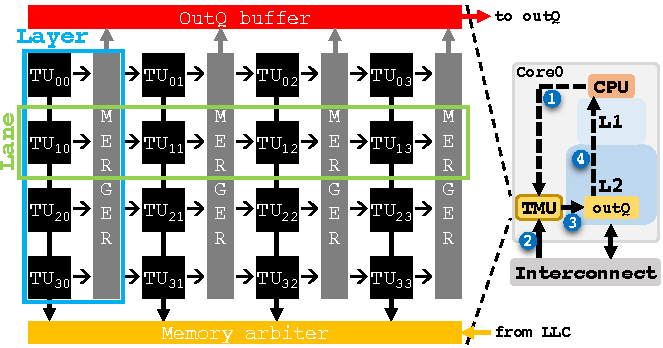
\includegraphics[width=.8\columnwidth]{img_engine_overview.pdf}
  \caption[TMU architecture and placement in a multicore processor.]{TMU architecture and placement in a multicore processor. Each core features its own TMU, which is placed nearby. Each TMU reads from the interconnect (last-level cache) and marshals data into the L2 cache of the core. Data read is managed by a memory arbiter whereas marshaling is managed by and output-queue (OutQ) buffer. The TMU is a matrix of Traversal Units (TUs), each one iterating through a linear space. Data flows from left to right. Multiple lanes (a row of TUs) allow to load data in parallel. Multiple layers (a column of TUs) allow to implement loop hierarchy, where data flows from left to right. Layers also allow for conjunctive and disjunctive merging of multiple tensor fibers.}
  \label{fig:engine_overview}
\end{figure}

We overcome the challenges discussed above by offloading critical tensor traversal and merging operations to a specialized unit, which we called the Tensor Marshaling Unit (TMU). This chapter introduces the TMU, its instruction set, its usage to accelerate sparse tensor algebra operations, its microarchitecture, and a comprehensive evaluation of its performance and power efficiency.

%%%%%%%%%%%%%%%%%%%%%%%%%%%%%%%%%%%%%%%%%%%%%%%%%%%%%%%%%%%%%%%%%%%%%%%%%%%%%%%%%%%%%%%%%%%%%%%%%%%%%%%%%%%%%%%%%%%%%%%%%%%%%%%%%%%
\section{TMU Architecture} \label{sec:tmu-architecture} %%%%%%%%%%%%%%%%%%%%%%%%%%%%%%%%%%%%%%%%%%%
%%%%%%%%%%%%%%%%%%%%%%%%%%%%%%%%%%%%%%%%%%%%%%%%%%%%%%%%%%%%%%%%%%%%%%%%%%%%%%%%%%%%%%%%%%%%%%%%%%%%%%%%%%%%%%%%%%%%%%%%%%%%%%%%%%%

This section introduces the TMU, its instruction set, and its usage to accelerate sparse tensor algebra operations.

%%%%%%%%%%%%%%%%%%%%%%%%%%%%%%%%%%%%%%%%%%%%%%%%%%%%%%%%%%%%%%%%%%%%%%%%%%%%%%%%%%%%%%%%%%%%%%%%%%%%%%%%%%%%%%%%%%%%%%%%%%%%%%%%%%%
\subsection{TMU Overview} \label{sec:tmu-overview} %%%%%%%%%%%%%%%%%%%%%%%%%%%%%%%%%%%%%%%%%%%
%%%%%%%%%%%%%%%%%%%%%%%%%%%%%%%%%%%%%%%%%%%%%%%%%%%%%%%%%%%%%%%%%%%%%%%%%%%%%%%%%%%%%%%%%%%%%%%%%%%%%%%%%%%%%%%%%%%%%%%%%%%%%%%%%%%

\Cref{fig:engine_overview} shows a general-purpose processor that features a TMU per core. Such system---which decouples memory access and computation in two separate units---is formally defined as a Decoupled Access-Execute (DAE) architecture. Overall, the TMU can be \textcircled{1} programmed to \textcircled{2} traverse and merge tensor operands and \textcircled{3} marshal the aggregated data to the core via a memory-mapped output queue (outQ) that the core can \textcircled{4} process. TMU traversal, merging, and marshaling is programmed with dataflow primitives whereas the compute code is wrapped in callback functions the TMU triggers on traversal/merging events.

\begin{figure}
\centering
  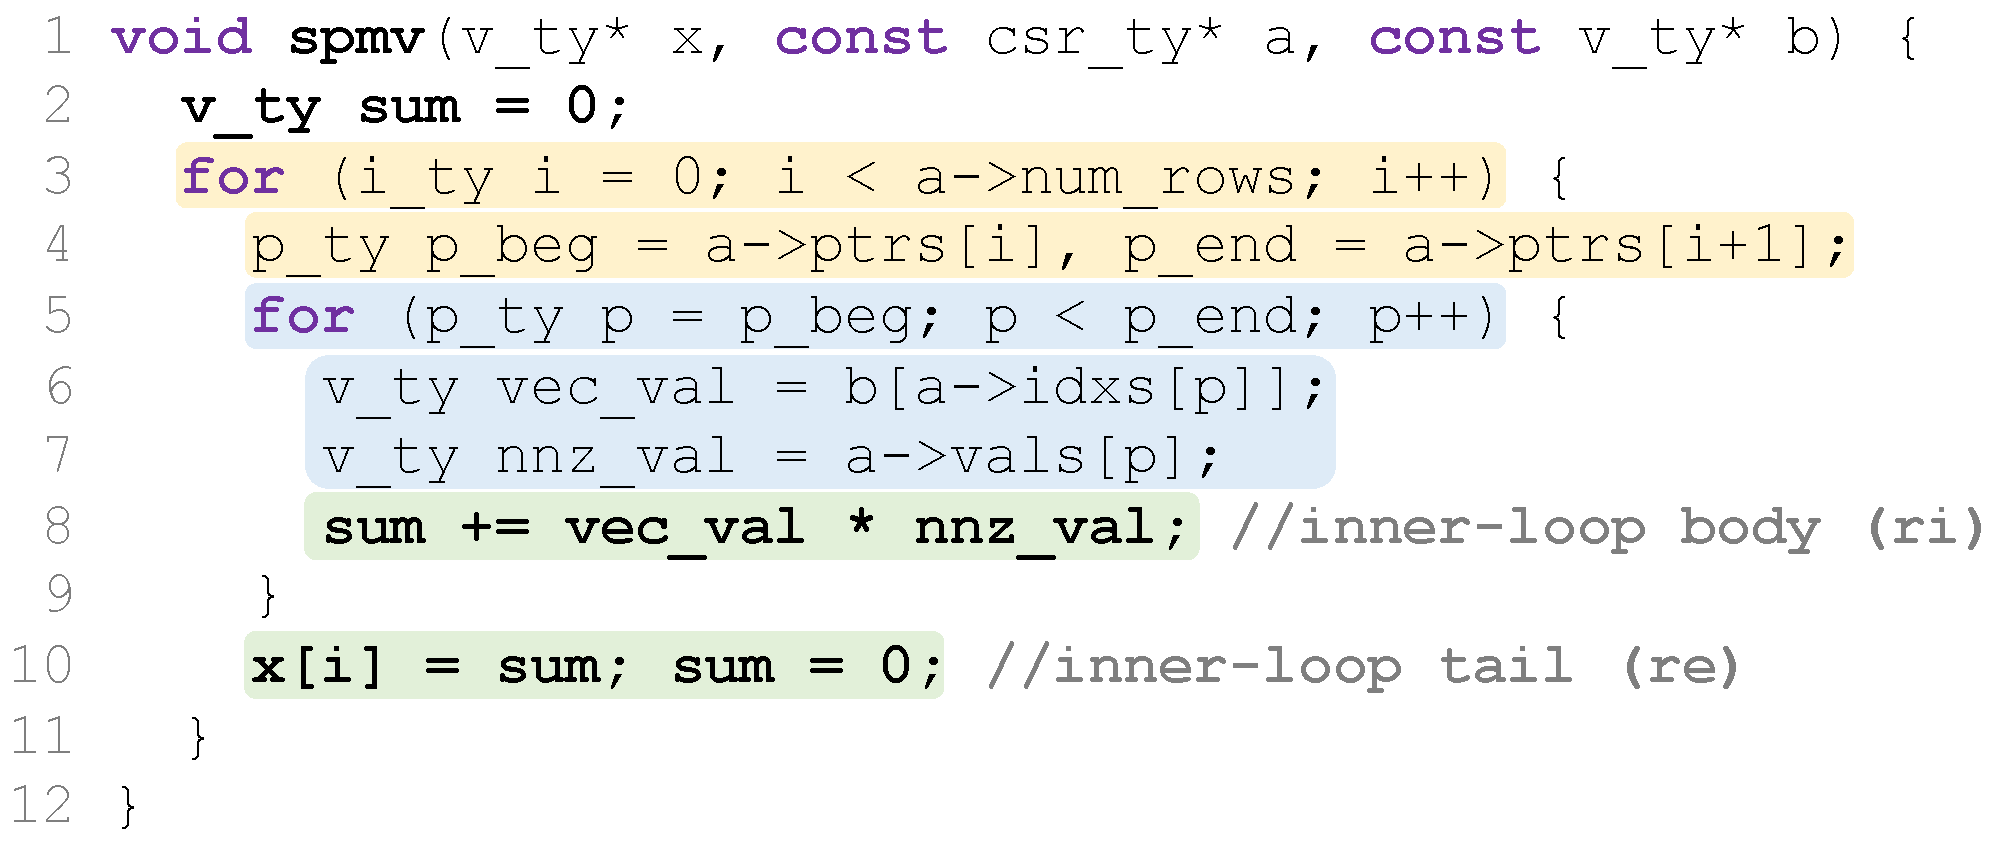
\includegraphics[width=.8\columnwidth]{img_spmv_decomposition.pdf}
  \caption[SpMV decomposition into fiber traversals and computation.]{SpMV decomposition in fiber traversals and computation. The outer-loop (lines 3-4 in yellow) traverses the dense CSR fiber of row pointers. The inner-loop traverses the compressed CSR fiber and dense vector with a scan-and-lookup operation (lines 5-7 in blue). Compute happens at the inner-loop body (line 8) and tail (line 10 in green).}
  \label{fig:spmv_decomposition}
\end{figure}

Because of the format abstraction described in \Cref{sec:tensor-compression-formats}, we can express tensor operations as \emph{dataflow} programs that stream input tensors through traversal, merging, and compute operations~\cite{sam2023asplos}. With this dataflow abstraction, we can map tensor traversal and merging to the TMU, and computation to the core. \Cref{fig:spmv_decomposition} shows this decomposition for SpMV.

\noindent\textbf{Traversal units, lanes and layers:}
As shown in \Cref{fig:engine_overview}, the TMU is a matrix of Traversal Units (TUs) where each TU implements logic and storage to traverse a tensor fiber, that is, each of the \texttt{for} loops in \Cref{fig:spmv_decomposition} (lines 3-4 and 5-7). Each of these \texttt{for} loops can be mapped to TUs of a TMU column, named \emph{layer}. The \texttt{for} loop in lines 3-4 would map to the left-most layer, producing indexes that flow into the second layer, where the \texttt{for} loop in lines 5-7 would be mapped. Therefore, the TMU has a dataflow design that flows rightward. In addition, loop iterations can be parallelized using multiple rows, named \emph{lanes}, which can also be used to load and merge multiple tensors.

\noindent\textbf{Multi-lane parallelism:} The values loaded by multiple lanes, either for parallel traversal or merging, are marshaled into vector operands. For example, each lane of the second layer that is traversing the \texttt{for} loop in lines 5-7 of \Cref{fig:spmv_decomposition} loads one \emph{vec\_val} and one \emph{nnz\_val}, which are then marshaled into vector operands.

\begin{figure}
\centering
  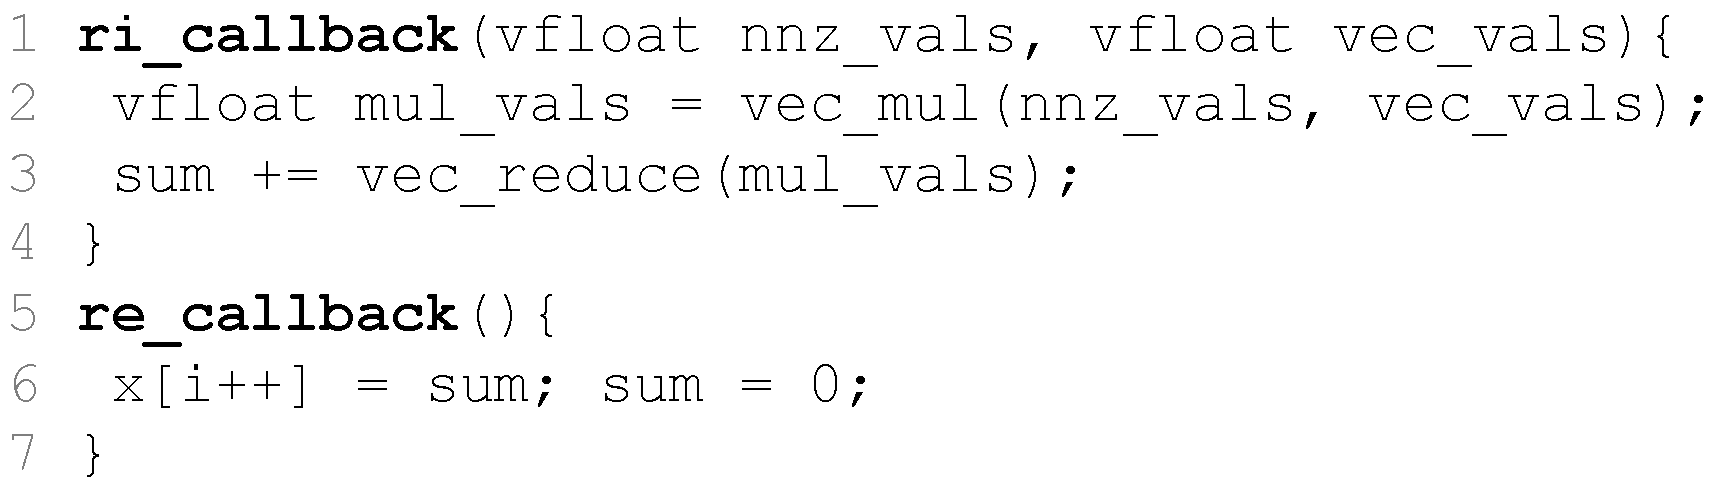
\includegraphics[width=.8\columnwidth]{img_spmv_cp_callbacks.pdf}
  \caption[SpMV callbacks.]{SpMV callbacks. The \texttt{ri} (row iteration) callback multiplies non-zero values with vector values, and accumulates them. The \texttt{re} (row end) callback writes back the accumulated value and initializes it.}
  \label{fig:spmv_cp_callbacks}
\end{figure}

\noindent\textbf{Callbacks and outQ processing:}
These operands are computed by the host core with the callbacks in \Cref{fig:spmv_cp_callbacks}.
These callbacks wrap the compute code of the body (\emph{ri}) and tail (\emph{re}) regions of the inner loop shown in \Cref{fig:spmv_decomposition}. The \emph{ri} callback accumulates partial-results (into the \texttt{sum} variable) and is triggered by the TMU at every row iteration (inner-loop body). The \emph{re} callback stores results at the end of every row traversal (inner-loop tail).
To decouple TMU and core execution, the TMU sends to the core, through the outQ, a control/data stream defining the ordered sequence of callbacks and operands that the core should compute.

For instance, running a 2-lanes SpMV on the CSR matrix in \Cref{fig:sparse_formats} would push in the outQ the following control/data sequence:
\begin{small}
\begin{verbatim}
ri AB ab ri C0 c0 re re ri DE cd re re ri FG de ri H0 f0 re
\end{verbatim}
\end{small}
triggering two accumulations for the first row, none for the second row (since empty), and so on.

The reminder of this section illustrates how to program the TMU to run parallel traversal/merging of Einsum expression.

%%%%%%%%%%%%%%%%%%%%%%%%%%%%%%%%%%%%%%%%%%%%%%%%%%%%%%%%%%%%%%%%%%%%%%%%%%%%%%%%%%%%%%%%%%%%%%%%%%%%%%%%%%%%%%%%%%%%%%%%%%%%%%%%%%%
\subsection{Tensor Traversal} \label{sec:tmu-traversal} %%%%%%%%%%%%%%%%%%%%%%%%%%%%%%%%%%%%%%%%%%%%%%%%%%%%%%%%%%%%%%%%%%%%%%%%%%%%%%%%
%%%%%%%%%%%%%%%%%%%%%%%%%%%%%%%%%%%%%%%%%%%%%%%%%%%%%%%%%%%%%%%%%%%%%%%%%%%%%%%%%%%%%%%%%%%%%%%%%%%%%%%%%%%%%%%%%%%%%%%%%%%%%%%%%%%

As described in \Cref{sec:tensor-traversal}, all sparse and dense fibers traversals have the following \texttt{for} loop structure:

{\small
\begin{verbatim}
    for(i=beg; i<end; i+=stride)
\end{verbatim}
}

Each TU provides the logic and storage to iterate such a loop, with \texttt{beg} and \texttt{end} defined by the fiber traversal, and load fiber values into streams.

%\begin{table}[htbp!]
\centering
\caption[TU traversal primitives.]{TU traversal primitives. For each signature, \texttt{int} arguments are constant values and \texttt{stream} arguments are the values loaded by the parent loop, as explained later.}
\label{tab:legacy-tmu-traversal-primitives}
\resizebox{\textwidth}{!}{%
\begin{tabular}{@{}llll@{}}
\toprule
\textbf{Type} & \textbf{Description} & \textbf{Signature} & \textbf{Traversal}\\
\midrule
\texttt{Dense} & dense (or singleton) fiber scan & \texttt{DnsFbrT(int beg, int end, int stride=1)} & for(i=beg; i<end; i+=stride)\\
\texttt{Range} & compressed fiber lookup and scan & \texttt{RngFbrT(stream beg, stream end, int offset=0, int stride=1)} & for(i=beg.head()+offset; i<end.head(); i+=stride)\\
\texttt{Index} & dense fiber lookup and scan & \texttt{IdxFbrT(stream beg, int size, int offset=0, int stride=1)} & for(i=beg.head()+offset; i<beg.head()+size; i+=stride)\\
\bottomrule 
\end{tabular}
}
\end{table}

%\begin{table}[htbp!]
\centering
\caption{Data streams for a TU.}
\label{tab:legacy-tmu-data-streams}
\begin{tabular}{@{}llc@{}}
\toprule
\textbf{Type} & \textbf{Description} & \textbf{Function}\\
\midrule
\texttt{mem} & loads \texttt{p}'s elements from memory at index \texttt{x} & \texttt{p[x]}\\
\texttt{ite} & generates TU iteration indices $\in$[\texttt{beg},\texttt{end}) & \texttt{x:b->e}\\
\texttt{lin} & implements a linear transformation on \texttt{x} & \texttt{ax+b}\\
\texttt{map} & reads \texttt{x}-th element of a small map \texttt{a=\{v1,...,v16\}} & \texttt{a[x]}\\
\texttt{ldr} & computes the address of the \texttt{x}-th element in \texttt{p} & \texttt{\&p[x]}\\
\midrule
\texttt{fwd} &\multicolumn{2}{l}{forwards a leftward TU stream to the next layer}\\
\texttt{msk} &\multicolumn{2}{l}{outputs a layer predicate for merging and lockstep operations}\\
\bottomrule 
\end{tabular}
\end{table}

%\begin{table}[htbp!]
\centering
\caption{Inter-layer configurations.}
\label{tab:legacy-tmu-layer-modes}
\begin{tabular}{@{}ll@{}}
\toprule
\textbf{Type} & \textbf{Description}\\
\midrule
\texttt{Single} & iterates a single lane\\
\texttt{BCast} & broadcasts a single lane to a parallel group\\
\texttt{Keep} & keeps one lane out of a parallel group\\
\midrule
\texttt{DisjMrg} & joins lanes of a layer\\
\texttt{ConjMrg} & intersects lanes of a layer\\
\texttt{LockStep} & co-iterates lanes of a layer\\
\bottomrule 
\end{tabular}
\end{table}

\begin{table}[htbp!]
\centering

% ---------- Table 3 ----------
\caption[TU traversal primitives.]{TU traversal primitives used to program fiber iteration. In each signature, \texttt{int} arguments are constants and \texttt{stream} arguments are values produced by a parent traversal. \texttt{Dense} implements a regular loop with static bounds, \texttt{Range} implements a loop with data-dependent bounds from streams, and \texttt{Index} implements a fixed-size dense lookup from a streamed base position. Overall, these primitives cover the loop-bound patterns needed for dense, compressed, and indirect traversal.}
\label{tab:tmu-traversal-primitives}
\resizebox{\textwidth}{!}{%
\begin{tabular}{@{}llll@{}}
\toprule
\textbf{Type} & \textbf{Description} & \textbf{Signature} & \textbf{Traversal}\\
\midrule
\texttt{Dense} & \makecell[l]{dense (or single)\\fiber scan} & \makecell[l]{\texttt{DnsFbrT(int beg, int end,}\\\texttt{ int stride=1)}} & \makecell[l]{for(i=beg; i<end;\\ \; i+=stride)}\\
\texttt{Range} & \makecell[l]{compressed fiber\\lookup and scan} & \makecell[l]{\texttt{RngFbrT(stream beg, stream end,}\\\texttt{ int offset=0, int stride=1)}} & \makecell[l]{for(i=beg.head()+offset;\\ \; i<end.head(); i+=stride)}\\
\texttt{Index} & \makecell[l]{dense fiber\\lookup and scan} & \makecell[l]{\texttt{IdxFbrT(stream beg, int size,}\\\texttt{ int offset=0, int stride=1)}} & \makecell[l]{for(i=beg.head()+offset;\\ \; i<beg.head()+size; i+=stride)}\\
\bottomrule
\end{tabular}
}

\vspace{1.2em}

% ---------- Table 4 ----------
\caption[TU data streams.]{Data streams produced or transformed by a TU. Memory streams load data using streamed indices, iteration and arithmetic streams generate addresses and loop positions, and forwarding or mask streams communicate values and predicates to the next layer. In this way, streams provide the dataflow interface between traversal, memory access, merging, and marshaling.}
\label{tab:tmu-data-streams}
\begin{tabular}{@{}llc@{}}
\toprule
\textbf{Type} & \textbf{Description} & \textbf{Function}\\
\midrule
\texttt{mem} & loads \texttt{p}'s elements from memory at index \texttt{x} & \texttt{p[x]}\\
\texttt{ite} & generates TU iteration indices $\in$[\texttt{beg},\texttt{end}) & \texttt{x:b->e}\\
\texttt{lin} & implements a linear transformation on \texttt{x} & \texttt{ax+b}\\
\texttt{map} & reads \texttt{x}-th element of a small map \texttt{a=\{v1,...,v16\}} & \texttt{a[x]}\\
\texttt{ldr} & computes the address of the \texttt{x}-th element in \texttt{p} & \texttt{\&p[x]}\\
\midrule
\texttt{fwd} &\multicolumn{2}{l}{forwards a leftward TU stream to the next layer}\\
\texttt{msk} &\multicolumn{2}{l}{outputs a layer predicate for merging and lockstep operations}\\
\bottomrule
\end{tabular}

\vspace{1.2em}

% ---------- Table 5 ----------
\caption[TMU inter-layer configurations.]{Inter-layer configurations used by Traversal Groups. \texttt{Single}, \texttt{BCast}, and \texttt{Keep} control how lanes are selected or broadcast, whereas \texttt{DisjMrg}, \texttt{ConjMrg}, and \texttt{LockStep} implement disjunctive merging, conjunctive merging, and lockstep co-iteration. In this way, these modes determine how lanes synchronize and how sparse fibers are merged across layers.}
\label{tab:tmu-layer-modes}
\begin{tabular}{@{}ll@{}}
\toprule
\textbf{Type} & \textbf{Description}\\
\midrule
\texttt{Single} & iterates a single lane\\
\texttt{BCast} & broadcasts a single lane to a parallel group\\
\texttt{Keep} & keeps one lane out of a parallel group\\
\midrule
\texttt{DisjMrg} & joins lanes of a layer\\
\texttt{ConjMrg} & intersects lanes of a layer\\
\texttt{LockStep} & co-iterates lanes of a layer\\
\bottomrule
\end{tabular}

\end{table}


\noindent\textbf{Fiber iteration:}
\Cref{tab:traversal} shows the primitives we can use to program TUs to implement the traversals in \Cref{sec:tensor-traversal}.
For instance, we can use a \texttt{Dense} primitive to implement the outer loop of SpMV in \Cref{fig:spmv_decomposition}, to iterate through matrix rows and load the row pointers.
These pointers, loaded into streams, are then used to implement the inner-loop traversal, with a \texttt{Range} primitive, to load non-zero values and column indexes (compressed levels), which, in turn, are used to load dense vector values through scan-and-lookup.
SpMM ($Z_{ij}=A_{ik}B_{kj}$), instead, works similarly but requires an additional inner loop, implemented with an \texttt{Indirect} primitive, to scan entire rows of the right-hand side matrix ($B_k$).

\noindent\textbf{Data loading:}
Once the iteration space of a TU is defined, data loading is implemented through the \emph{data streams} listed in \Cref{tab:streams}.
The \texttt{mem} stream loads data from a base address and a stream of indexes.
To generate the index stream, TUs push their current iteration index (i.e., loop induction variable) into an \texttt{ite} stream, which can also be transformed with \texttt{lin} or \texttt{map} streams. Indirect accesses can be implemented by chaining \texttt{mem} streams.
Hence, we can represent a fiber traversal with a \textit{parent}-\textit{children} dependency tree where the \texttt{ite} stream is the \textit{root}.
For instance, the SpMV scan-and-lookup operation in \Cref{fig:spmv_decomposition} is implemented by instantiating two \texttt{mem} streams: a parent stream that loads the column indexes which are then used by its child stream to index into the dense vector.

%%%%%%%%%%%%%%%%%%%%%%%%%%%%%%%%%%%%%%%%%%%%%%%%%%%%%%%%%%%%%%%%%%%%%%%%%%%%%%%%%%%%%%%%%%%%%%%%%%%%%%%%%%%%%%%%%%%%%%%%%%%%%%%%%%%
\subsection{Tensor Merging and Vectorization} \label{sec:tmu-merging} %%%%%%%%%%%%%%%%%%%%%%%%%%%%%%%%%%%%%%%%%%%%%%%%%%%%%%%%%%%%%%%%
%%%%%%%%%%%%%%%%%%%%%%%%%%%%%%%%%%%%%%%%%%%%%%%%%%%%%%%%%%%%%%%%%%%%%%%%%%%%%%%%%%%%%%%%%%%%%%%%%%%%%%%%%%%%%%%%%%%%%%%%%%%%%%%%%%%

We can use multiple TMU lanes to parallelize loop traversal or merge different tensors.
Parallelization and merging can happen at any tensor level by setting TMU layers to one of the configurations shown in \Cref{tab:tg_config}. 

\noindent\textbf{Parallelization} is achieved by parallelizing loop iterations by using different lanes.
Overall, parallelization allows (1) parallel loading, reducing the control overhead of traversing compressed data structures, and (2) parallel marshaling, enabling efficient vectorized compute in the host core.
The bi-dimensional TMU design allows to parallelize loops at different levels.
For instance, inner-loop parallelization allows to marshal adjacent tensor elements in the same vector operand (i.e. usual vectorization scheme).
Outer-loop parallelization, instead, allows to marshal multiple fibers, slices, and arbitrary tensor dimensions in the same vector operand, enabling higher-dimensional parallelization schemes.
In the SpMV example in \Cref{fig:spmv_decomposition}, where we parallelize at the inner-loop level, we should configure the first layer to load row pointers and \texttt{BCast} them to the next layer to load multiple elements of the same row in \texttt{LockStep} (with each lane loading at a different offset).
To parallelize SpMV at the outer-loop level, concurrently loading multiple rows into different lanes, both layers should work in \texttt{LockStep}.
Both parallization schemes aggregate data into vector operands that are marshaled into the core for computation.
Boundary conditions can be handled by padding or marshaling the \texttt{msk} stream along with the operands, indicating the active elements in a multi-hot bit vector (equivalent to the \texttt{svwhilelt} operation in Arm SVE~\cite{sve2017micro}).

\begin{figure}
\centering
  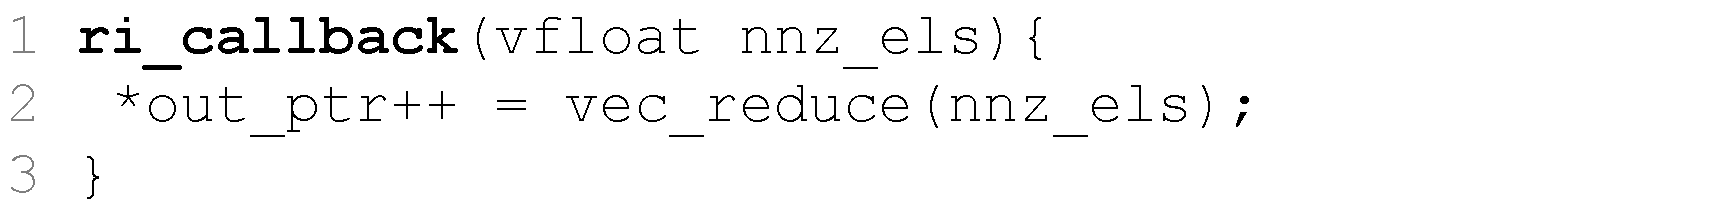
\includegraphics[width=.8\columnwidth]{img_spkadd_callbacks.pdf}
  \caption[SpKAdd callback.]{SpKAdd callback. It just reduces all vector elements.}
  \label{fig:spkadd_callbacks}
\end{figure}

\noindent\textbf{Fiber merging} is achieved by loading different tensors in different lanes and merging them hierarchically with the mergers placed between layers.
Merging operations are implemented by "sorting" the fiber indexes of all the active lanes in the layers, which is achieved by iteratively pulling fibers with minimum indexes.
The position of these fibers can be identified with a multi-hot $l$-bit predicate, which is pushed in the \texttt{msk} stream of the layer.
For the 2-lane merging example in \Cref{fig:merging}, the \texttt{msk} stream is \texttt{11, 01, 10, 11}, with first bit representing fiber A, second bit fiber B.
These predicates are then used to aggregate vector operands to send to the core.
In this way, for instance, we can implement SpKAdd~\cite{hussain2022spkadd}, a summation of K sparse matrices, by mapping matrices in K different lanes and merging them with \texttt{DisjMrg} layers.
\Cref{fig:spkadd_callbacks} shows the compute code of SpKAdd: the TMU traverses all the K matrices row by row and, for each row, sends to the core all non-zero values with the same index, which are reduced with a vector operation.
Running SpKAdd on the two rows in \Cref{fig:merging} would produce the following vector operand stream: \texttt{AB C D EF}, with \texttt{AB} and \texttt{EF} being reduced in the core.
If matrices are in CSR format, only the second compressed dimension requires merging.
In contrast, if matrices are in DCSR format, both dimensions are compressed and both need to be merged.
In this latter case, the merge happens hierarchically: only the active lanes from the first dimension, which are identified by the \texttt{msk} predicate of the first layer, are merged in the second layer.

%%%%%%%%%%%%%%%%%%%%%%%%%%%%%%%%%%%%%%%%%%%%%%%%%%%%%%%%%%%%%%%%%%%%%%%%%%%%%%%%%%%%%%%%%%%%%%%%%%%%%%%%%%%%%%%%%%%%%%%%%%%%%%%%%%%
\subsection{Data Marshaling and Computation} \label{sec:marshaling-and-computation} %%%%%%%%%%%%%%%%%%%%%%%%%%%%%%%%%%%%%%%%%%%%%%%%%%%
%%%%%%%%%%%%%%%%%%%%%%%%%%%%%%%%%%%%%%%%%%%%%%%%%%%%%%%%%%%%%%%%%%%%%%%%%%%%%%%%%%%%%%%%%%%%%%%%%%%%%%%%%%%%%%%%%%%%%%%%%%%%%%%%%%%

Once we mapped the loop structure of a tensor expression into TMU layers, the TMU streams the aggregated data to the core for computation. Core compute is enabled by wrapping into callback functions the compute code within the \textit{head} (H), \textit{body} (B), and \textit{tail} (T) regions of traversal/merging loops. % of a tensor expression.
These callback functions have a unique callback ID and a list of scalar, vector, or predicate operands produced by the TMU.
In the SpMV example in \Cref{fig:spmv_decomposition}, we wrap the code in the inner-loop body into a \texttt{ri} callback, which multiplies and accumulates the matrix and vector values provided by the TMU, and the code in the inner-loop tail into a \texttt{re} callback, to store the accumulated results.

Each layer of the TMU is programmed to trigger these callbacks upon traversal/merging events such as the \textit{begin}, \textit{iteration}, and \textit{end} of a traversal or merging.
In the SpMV example in \Cref{fig:spmv_decomposition}, we register the \texttt{ri} callback to the \textit{iteration} of the inner-loop layer and the \texttt{re} callback to the \textit{end} of the inner-loop layer.
For the \texttt{ri} callback, we also register the list of operands consisting of matrix and vector values. Callback registration can be done with the following callback:

{\small
\begin{verbatim}
    add_callback(event, callback_id, args_list)
\end{verbatim}
}

While running, the TMU pushes the callback IDs and vector operands of each registered event into the current outQ chunk.
When the chunk is full, the core starts reading callback IDs and executes the proper HBT callback to compute the data operands.
Meanwhile, the TMU populates another outQ chunk, overlapping data loading and computation.

%%%%%%%%%%%%%%%%%%%%%%%%%%%%%%%%%%%%%%%%%%%%%%%%%%%%%%%%%%%%%%%%%%%%%%%%%%%%%%%%%%%%%%%%%%%%%%%%%%%%%%%%%%%%%%%%%%%%%%%%%%%%%%%%%%%
\subsection{Mapping Sparse Tensor Algebra Operations to the TMU} \label{sec:mapping} %%%%%%%%%%%%%%%%%%%%%%%%%%%%%%%%%%%%%%%%%%%%%%%%%%%%%%%%%%%
%%%%%%%%%%%%%%%%%%%%%%%%%%%%%%%%%%%%%%%%%%%%%%%%%%%%%%%%%%%%%%%%%%%%%%%%%%%%%%%%%%%%%%%%%%%%%%%%%%%%%%%%%%%%%%%%%%%%%%%%%%%%%%%%%%%

\begin{figure}
\centering
  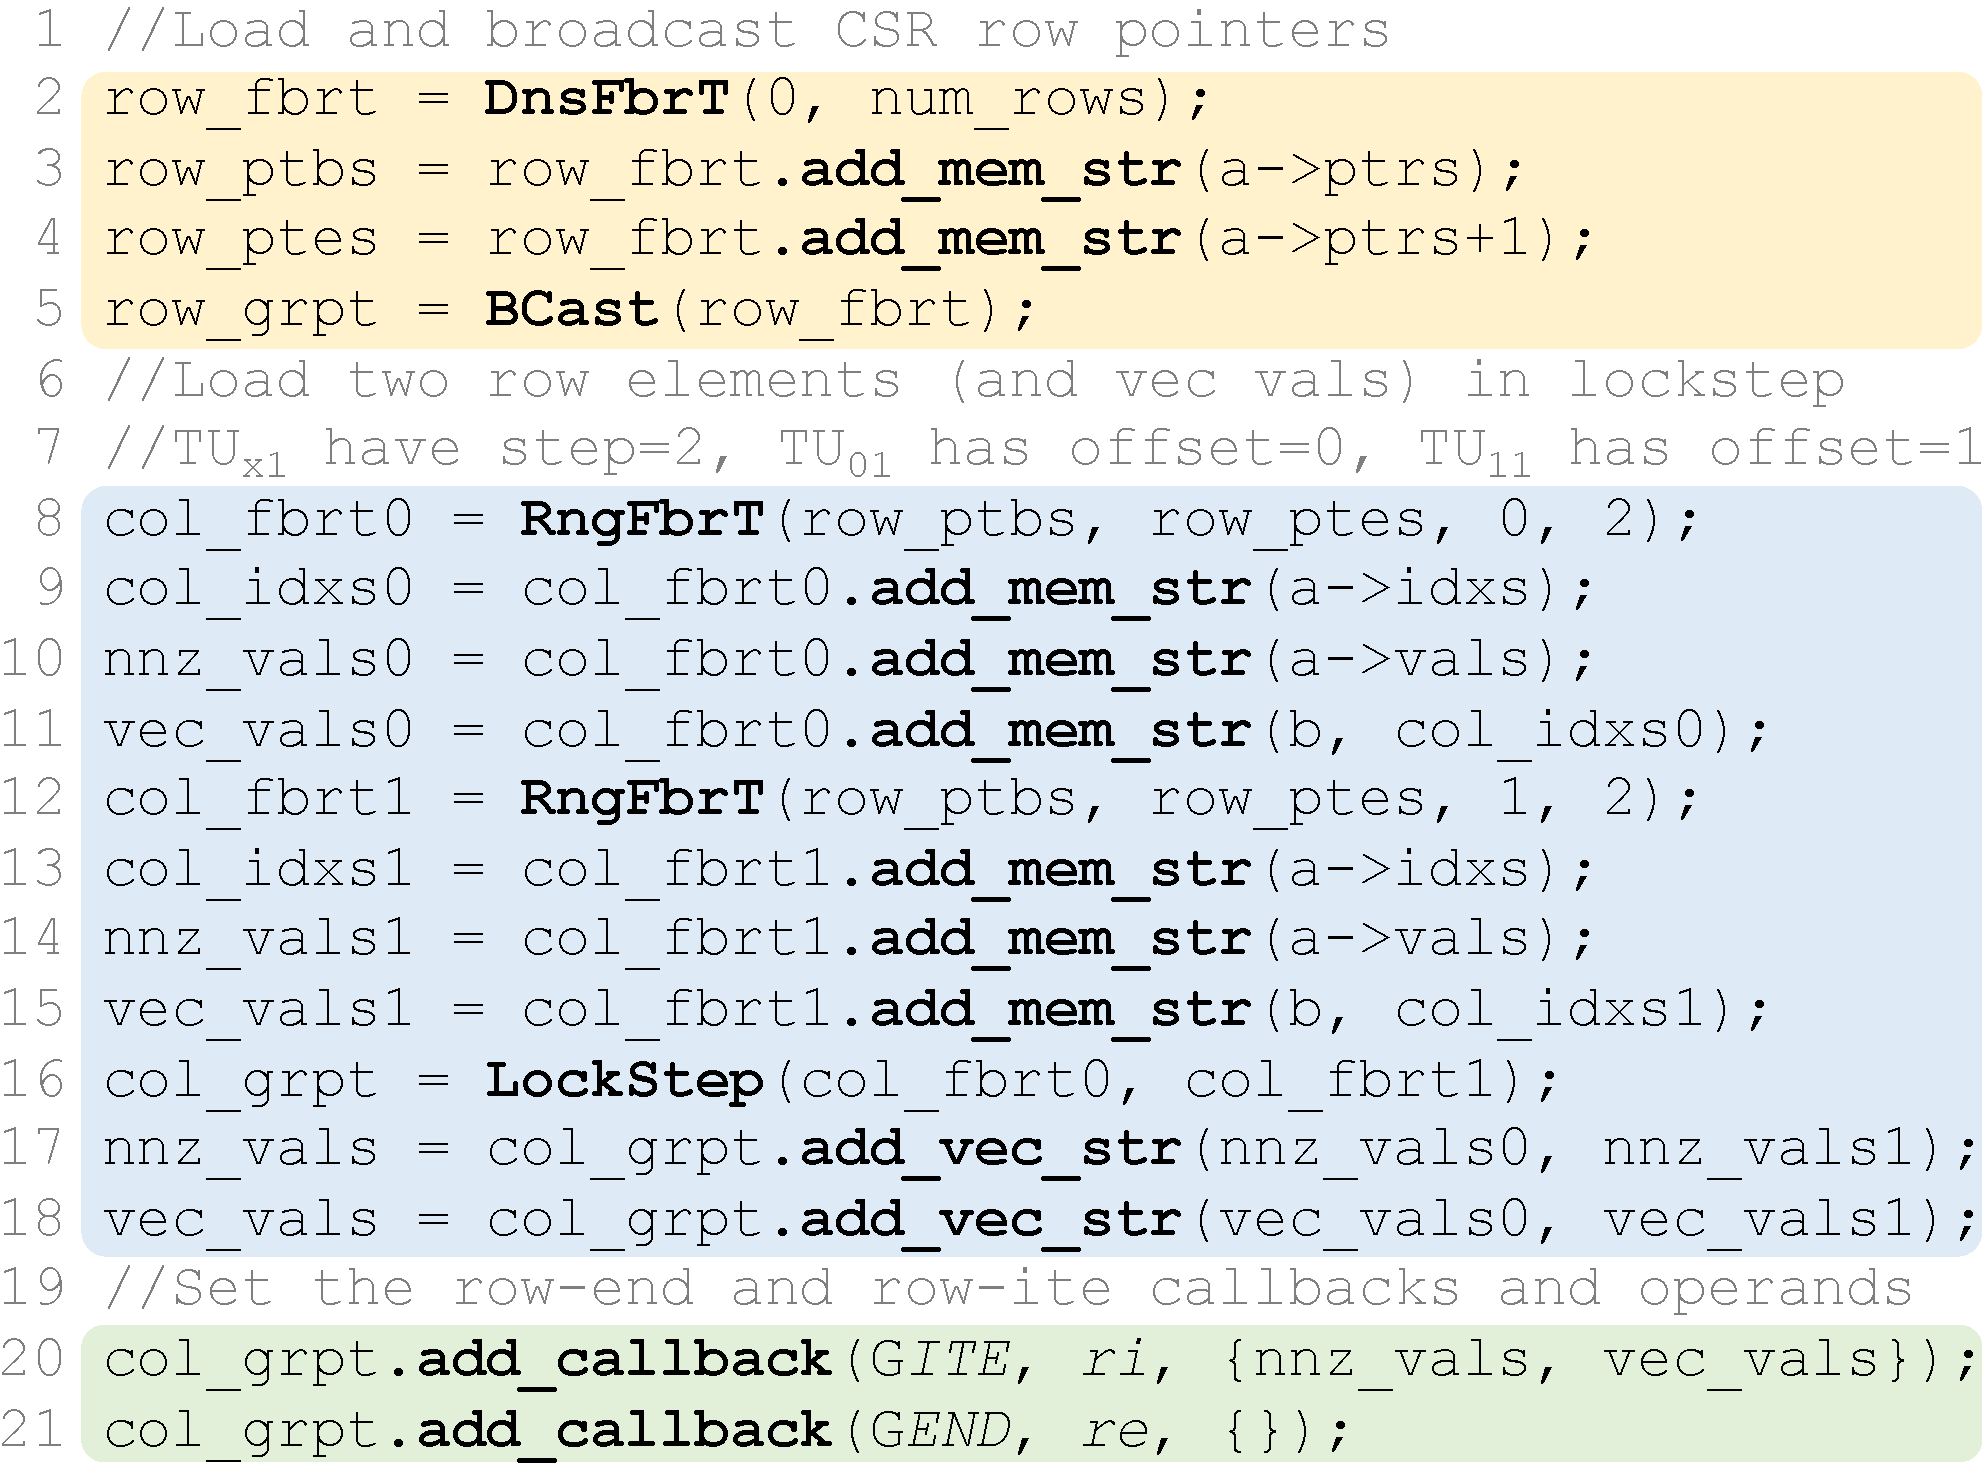
\includegraphics[width=.8\columnwidth]{img_spmv_programmability.pdf}
  \caption[TMU code for SpMV column-parallel.]{TMU code for SpMV column-parallel. Colors match \Cref{fig:spmv_decomposition} to highlight mapping.}
  \label{fig:spmv_programmability}
\end{figure}

\begin{sidewaystable}
    \centering
    \setlength{\tabcolsep}{2.5pt}
    \caption[Mapping sparse tensor algebra kernels to TMU hardware.]{Mapping sparse tensor algebra kernels to TMU hardware. Each row lists an Einsum expression, sparse input formats, a loop schedule, the traversal primitives, data streams, inter-layer modes, and callbacks needed to execute that kernel on the TMU. Underlined schedule indices identify the loop level parallelized across lanes (notation P\textit{x}). Thus, the table shows that the same TMU primitives cover sparse-dense traversal, sparse-sparse merging, vectorization, and callback generation across a broad set of kernels.}
    \label{tab:tmu-tensor-algebra-mapping}
    \resizebox{\textwidth}{!}{%
    \begin{tabular}{@{}lllc|ccc|cccccc|cccccc|ccc@{}}
    \toprule
        \multirow{2}{*}{\textbf{Algorithm}} & \textbf{Einsum} & \textbf{Sparse} & \textbf{Schedule} & \multicolumn{3}{c|}{\textbf{Traversal type}} & \multicolumn{6}{c|}{\textbf{Data streams}} & \multicolumn{6}{c|}{\textbf{Group Traversal}} & \multicolumn{3}{c}{\textbf{Callbacks}} \\ 
        
        & \textbf{expression} & \textbf{formats} & \textbf{(\underline{SIMD})} & \textbf{Dns} & \textbf{Idx} & \textbf{Rng} & \textbf{lin} & \textbf{map} & \textbf{mem} & \textbf{ldr} & \textbf{fwd} & \textbf{msk} & \textbf{Single} & \textbf{BCast} & \textbf{LockStep} & \textbf{CnjMrg} & \textbf{DsjMrg} & \textbf{Keep} & \textbf{H} & \textbf{B} & \textbf{T} \\ \midrule
        \textbf{SpMV P0} & $Z_i=A_{ij}B_j$ & $A$=CSR & $\underline{ij}$ & $i$ & ~ & $j$ & ~ & ~ & $ij$ & ~ & ~ & ~ & ~ & ~ & $ij$ & ~ & ~ & ~ & ~ & $j$ & ~ \\
        \textbf{SpMV P1} & $Z_i=A_{ij}B_j$ & $A$=CSR & $i\underline{j}$ & $i$ & ~ & $j$ & ~ & ~ & $ij$ & ~ & ~ & ~ & ~ & $i$ & $j$ & ~ & ~ & ~ & ~ & $j$ & $j$ \\
        \textbf{SpMSpV} & $Z_i=A_{ij}B_j$ & $A$,$B$=CSR & $ij$ & $ij$ & ~ & $j$ & ~ & ~ & $ij$ & ~ & ~ & ~ & ~ & $i$ & ~ & $j$ & ~ & ~ & ~ & $j$ & ~ \\
        \textbf{SpMM P0} & $Z_{ij}=A_{ik}B_{kj}$ & $A$=CSR & $\underline{ikj}$ & $ij$ & $j$ & $k$ & ~ & ~ & $ikj$ & ~ & ~ & ~ & ~ & ~ & $ikj$ & ~ & ~ & ~ & $j$ & $j$ & ~ \\
        \textbf{SpMM P1} & $Z_{ij}=A_{ik}B_{kj}$ & $A$=CSR & $i\underline{kj}$ & $ij$ & $j$ & $k$ & ~ & ~ & $ikj$ & ~ & ~ & ~ & ~ & $i$ & $kj$ & ~ & ~ & ~ & $j$ & $j$ & $k$ \\
        \textbf{SpMM P2} & $Z_{ij}=A_{ik}B_{kj}$ & $A$=CSR & $ik\underline{j}$ & $ij$ & $j$ & $k$ & ~ & ~ & $ikj$ & ~ & ~ & ~ & $i$ & $k$ & $j$ & ~ & ~ & ~ & $j$ & $j$ & ~ \\
        \textbf{SpMSpM P0} & $Z_{ij}=A_{ik}B_{kj}$ & $A$,$B$,$X$=CSR & $\underline{ikj}$ & $i$ & ~ & $kj$ & ~ & ~ & $ikj$ & ~ & ~ & ~ & ~ & ~ & $ikj$ & ~ & ~ & ~ & ~ & $j$ & $k$ \\
        \textbf{SpMSpM P2} & $Z_{ij}=A_{ik}B_{kj}$ & $A$,$B$,$X$=CSR & $ik\underline{j}$ & $i$ & ~ & $kj$ & ~ & ~ & $ikj$ & ~ & ~ & ~ & $i$ & $k$ & $j$ & ~ & ~ & ~ & $j$ & $j$ & $k$ \\
        \textbf{SpKAdd} & $Z_{ij}=\sum_{k}^{}A^{k}_{ij}$ & $A^{k}$,$X$=DCSR & $\underline{kij}$ & $i$ & ~ & $j$ & ~ & ~ & $ij$ & ~ & ~ & $j$ & ~ & ~ & ~ & ~ & $ij$ & ~ & ~ & $j$ & ~ \\
        \textbf{PageRank} & $Z_i=A_{ij}X_jY_i$ & $A$=CSR & $i\underline{j}$ & $i$ & ~ & $j$ & ~ & ~ & $ij$ & ~ & ~ & ~ & ~ & $i$ & $j$ & ~ & ~ & ~ & ~ & $j$ & $j$ \\
        \textbf{TriangleCount} & $c=L_{ik}L^{T}_{kj}L_{ij}$ & $L$=CSR & $ikj$ & $i$ & ~ & $kj$ & ~ & ~ & $ikj$ & ~ & $k$ & ~ & ~ & ~ & $ik$ & $j$ & ~ & ~ & ~ & $j$ & ~ \\
        \textbf{MTTKRP P1} & $Z_{ij} = A_{ikl}B_{kj}C_{lj}$ & $A$=COO & $i\underline{klj}$ & $ij$ & $klj$ & ~ & $i$ & ~ & $iklj$ & ~ & ~ & ~ & ~ & $i$ & $klj$ & ~ & ~ & ~ & $j$ & $j$ & ~ \\
        \textbf{MTTKRP P2} & $Z_{ij} = A_{ikl}B_{kj}C_{lj}$ & $A$=COO & $ikl\underline{j}$ & $iklj$ & $j$ & ~ & $i$ & $kl$ & $iklj$ & $i$ & ~ & ~ & $i$ & $kl$ & $j$ & ~ & ~ & ~ & $kl$ & $j$ & ~ \\
        \textbf{SpTC} & $Z_{ij} = A_{ikl}B_{lkj}$ & $A$,$B$=CSF & $iklj$ & $i$ & ~ & $jkl$ & ~ & ~ & $ijkl$ & ~ & ~ & ~ & ~ & $i$ & ~ & $jkl$ & ~ & $j$ & ~ & $j$ & $i$ \\
        \textbf{SpTTV} & $Z_{ij} = A_{ijk}B_{k}$ & $A$=CSF & $ij\underline{k}$ & $ik$ & ~ & $jk$ & ~ & ~ & $ijk$ & ~ & ~ & ~ & ~ & $k$ & $k$ & ~ & ~ & ~ & ~ & $k$ & $k$ \\
        \textbf{SpTTM} & $Z_{ijk} = A_{ijl}B_{lk}$ & $A$=CSF & $ijl\underline{k}$ & $ik$ & $l$ & $jl$ & ~ & ~ & $ijlk$ & ~ & ~ & ~ & ~ & $l$ & $k$ & ~ & ~ & ~ & ~ & $k$ & $k$ \\
        \bottomrule
    \end{tabular}}    
\end{sidewaystable}


\Cref{fig:spmv_programmability} shows the full TMU configuration code for the SpMV example in \Cref{fig:spmv_decomposition}.
The top block defines the dense traversal (\emph{DnsFbrT}) for the CSR matrix row pointers.
The middle block (second layer) co-iterates in \emph{LockStep} two columns in parallel (\emph{RngFbrT}), marshaling vector operands to the core (lines 17 and 18).
The bottom block registers the \emph{callbacks} happening at each row iteration (\textit{ri}), specifying the associated data, and at the end of a row (\textit{re}).

\Cref{tab:tensor-mapping} has an extensive list of tensor algebra algorithms showing how they map to the TMU. The loop schedule encodes the different parallelization schemes by underlining the parallel loops generating vector operands. Additionally, for each loop we state: (i) traversal type, (ii) instantiated data streams, (iii) layer operation mode, and (iv) associated callbacks.
To prove functional completeness of TMU primitives with respect to tensor algebra, we observe that our primitives implement all of the minimal functionalities for tensor algebra formulated by Hsu et al.~\cite{sam2023asplos}.

%%%%%%%%%%%%%%%%%%%%%%%%%%%%%%%%%%%%%%%%%%%%%%%%%%%%%%%%%%%%%%%%%%%%%%%%%%%%%%%%%%%%%%%%%%%%%%%%%%%%%%%%%%%%%%%%%%%%%%%%%%%%%%%%%%%
\section{TMU Microarchitecture} \label{sec:tmu-microarchitecture} %%%%%%%%%%%%%%%%%%%%%%%%%%%%%%%%%%%%%%%%%%%%%%%%%%%%%%%%%%%%%%%%%
%%%%%%%%%%%%%%%%%%%%%%%%%%%%%%%%%%%%%%%%%%%%%%%%%%%%%%%%%%%%%%%%%%%%%%%%%%%%%%%%%%%%%%%%%%%%%%%%%%%%%%%%%%%%%%%%%%%%%%%%%%%%%%%%%%%

This chapter details the TMU microarchitecture as well as the implementation and operation of its components. We conclude with a step-by-step example.

%%%%%%%%%%%%%%%%%%%%%%%%%%%%%%%%%%%%%%%%%%%%%%%%%%%%%%%%%%%%%%%%%%%%%%%%%%%%%%%%%%%%%%%%%%%%%%%%%%%%%%%%%%%%%%%%%%%%%%%%%%%%%%%%%%%
\subsection{Traversal Unit Design} \label{sec:traversal-unit-design} %%%%%%%%%%%%%%%%%%%%%%%%%%%%%%%%%%%%%%%%%%%%%%%%%%%%%%%%%%%%%%%%%%%%%%%%%%%%%%%%%%%%%%%%%%%%%%%%%%%
%%%%%%%%%%%%%%%%%%%%%%%%%%%%%%%%%%%%%%%%%%%%%%%%%%%%%%%%%%%%%%%%%%%%%%%%%%%%%%%%%%%%%%%%%%%%%%%%%%%%%%%%%%%%%%%%%%%%%%%%%%%%%%%%%%%

TUs implement the logic to (i)~iterate tensor fibers, (ii)~generate a binary control sequence to track the iteration status, and (iii)~populate data streams.
To iterate a tensor fiber, each TU implements a finite-state machine (FSM) looping through the \texttt{fbeg}, \texttt{fite}, and \texttt{fend} states.
The \texttt{fbeg} state initializes the iteration boundaries, which can either be constant values or read from a leftward TU, stalling the current TU execution if the leftward TU has not produced new valid data yet.
If the streams, which are implemented as circular queues, are not full, the \texttt{fite} state pushes (i)~a \texttt{0} token into the binary control sequence, (ii)~the current iteration index into the \texttt{ite} stream, and (iii)~a new element into each other stream (which is generated according to the stream type).
As discussed below, the value of this element depends on its input queue.
Finally, when the fiber traversal has no more elements to iterate, the \texttt{fend} state pushes a \texttt{1} token into the binary control sequence and goes back to the \texttt{fbeg} state.

All data streams within the same TU are of equal size and controlled simultaneously with a single push/pull command.
Hence, the value of the \textit{i}-th element of a queue is computed starting from the \textit{i}-th element of its parent queue, as defined in \Cref{sec:tmu-traversal}.
In case the parent queue implements a \texttt{mem} stream, because of memory latency, its value may not be available immediately, leaving some queue elements in a transient state. In particular, queue elements can either be in a \texttt{valid} or \texttt{waiting} state according to whether the status of the corresponding element in the parent queue is valid or not, respectively. Elements of \texttt{mem} queues, instead, can be in a \texttt{waiting}, \texttt{queued}, \texttt{requested}, or \texttt{valid} state according to whether the parent index is not valid, the address got computed, the request got submitted to memory, or the data got back, respectively.

%%%%%%%%%%%%%%%%%%%%%%%%%%%%%%%%%%%%%%%%%%%%%%%%%%%%%%%%%%%%%%%%%%%%%%%%%%%%%%%%%%%%%%%%%%%%%%%%%%%%%%%%%%%%%%%%%%%%%%%%%%%%%%%%%%%
\subsection{Traversal Group Design} \label{sec:traversal-group-design} %%%%%%%%%%%%%%%%%%%%%%%%%%%%%%%%%%%%%%%%%%%%%%%%%%%%%%%%%%%%%%%%%%%%%%%%%%%%%%%%%%%%%%%%%%%%%%%%%%
%%%%%%%%%%%%%%%%%%%%%%%%%%%%%%%%%%%%%%%%%%%%%%%%%%%%%%%%%%%%%%%%%%%%%%%%%%%%%%%%%%%%%%%%%%%%%%%%%%%%%%%%%%%%%%%%%%%%%%%%%%%%%%%%%%%

A Traversal Group (TG) implements the logic to merge and co-iterate TUs in a layer. 
Similarly to TUs, TGs also implement an FSM to loop through \texttt{gbeg}, \texttt{gite}, and \texttt{gend} states, generating predicates and a control sequence used later on to trigger callbacks.
TG FSMs compute their control sequence by combining (i) the predicate of the previous layer, if any, and (ii) the control sequences of all the TUs in the layer, implementing a hierarchical evaluation.
In particular, we consider a lane to be \emph{active} only if the corresponding bit of the predicate coming out of the previous layer is set to true.
TGs only process a \texttt{gite} state if all the active lanes have valid data in their queue heads.

In case of disjunctive merging, the \texttt{gite} state (i) computes the output predicate by setting to \texttt{1} the active lanes with minimum indexes, (ii) consumes them, and (iii) pushes a \texttt{0} token into the binary control sequence.
When all active TUs have no more elements to merge disjunctively, the \texttt{gend} state pushes a \texttt{1} token into the binary control sequence.


\begin{figure}
    \centering
    \begin{subfigure}[b]{\textwidth}
        \centering
        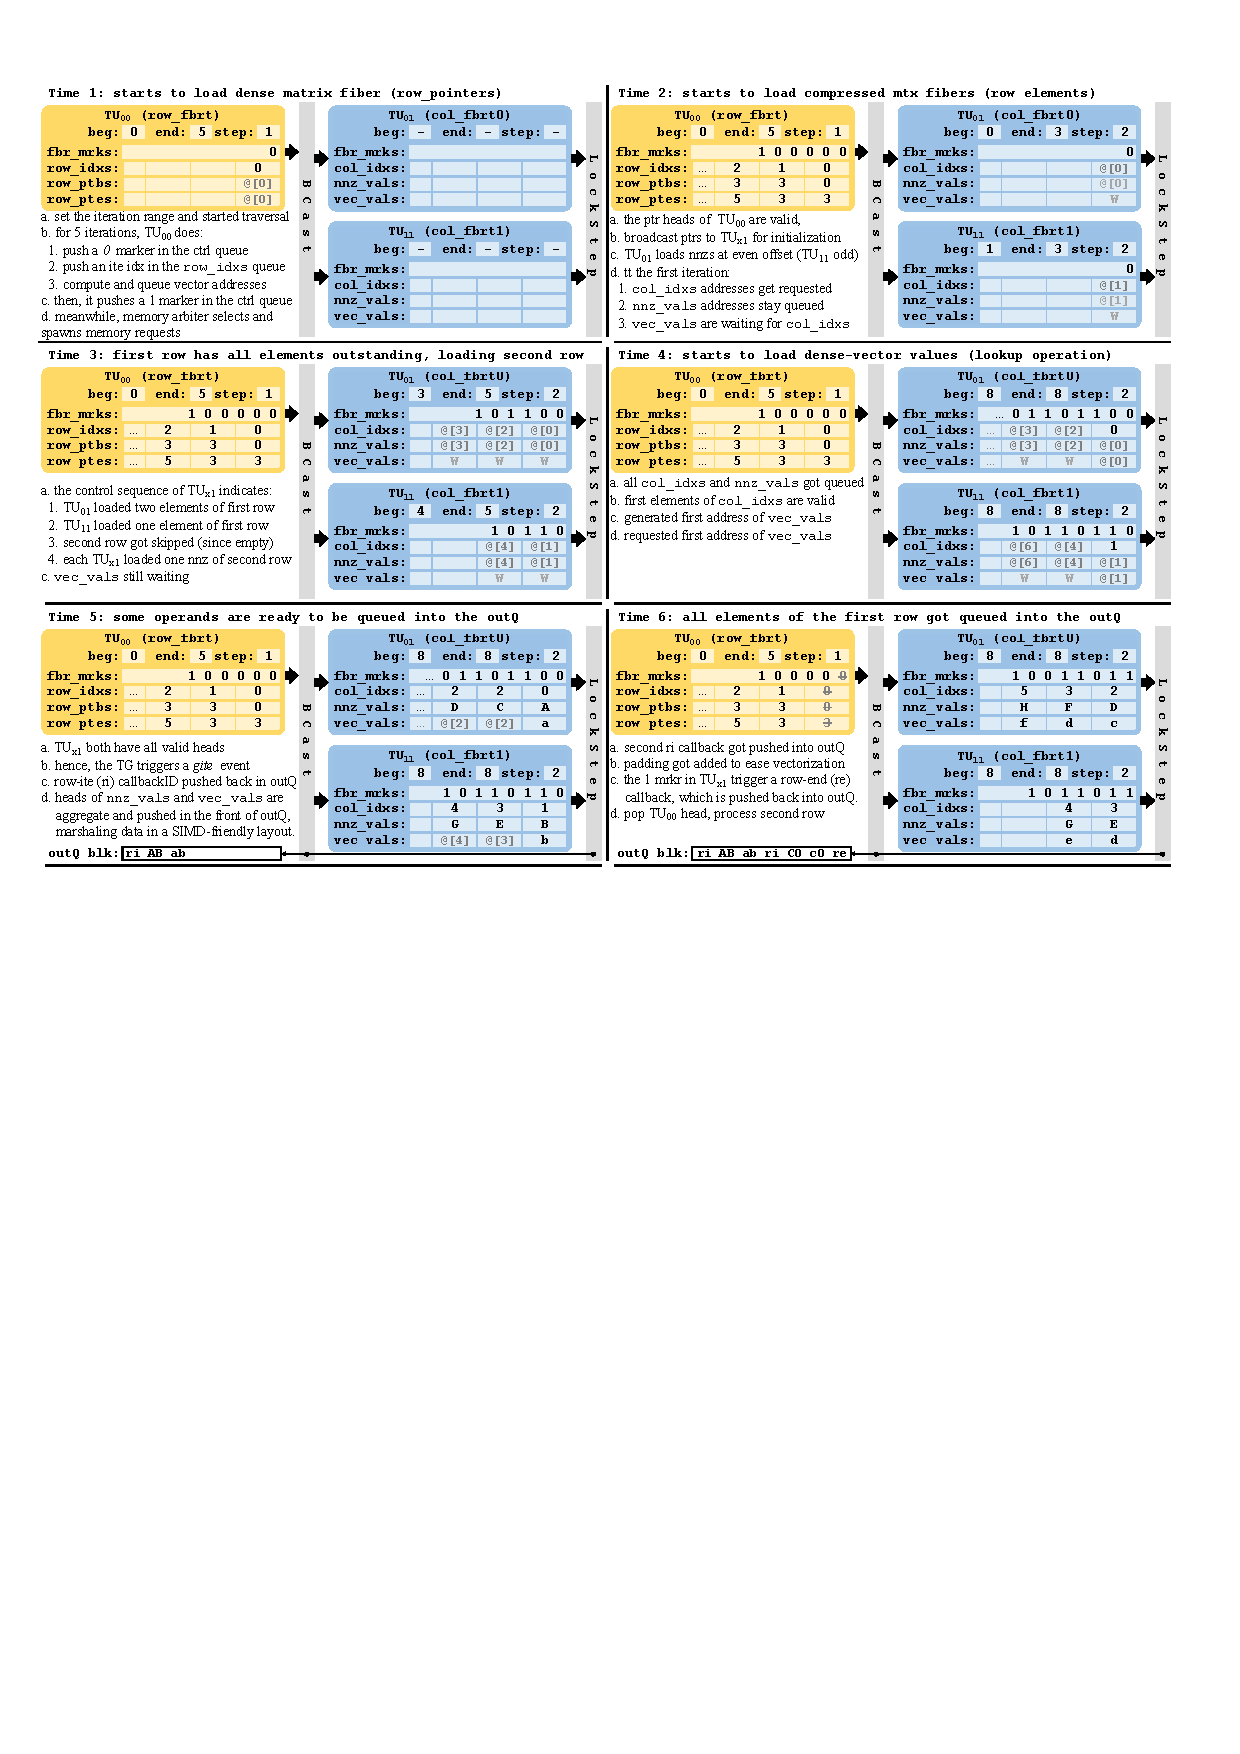
\includegraphics[width=\textwidth,trim=0 260 275 10,clip]{img_spmv_sbs_example.pdf}
        \vspace{-0.5cm}
        \caption{T1: starts to load dense matrix fiber (row\_pointers)}
        \label{fig:sbs-example-t1}
    \end{subfigure}
    \centering
    \begin{subfigure}[b]{\textwidth}
        \centering
        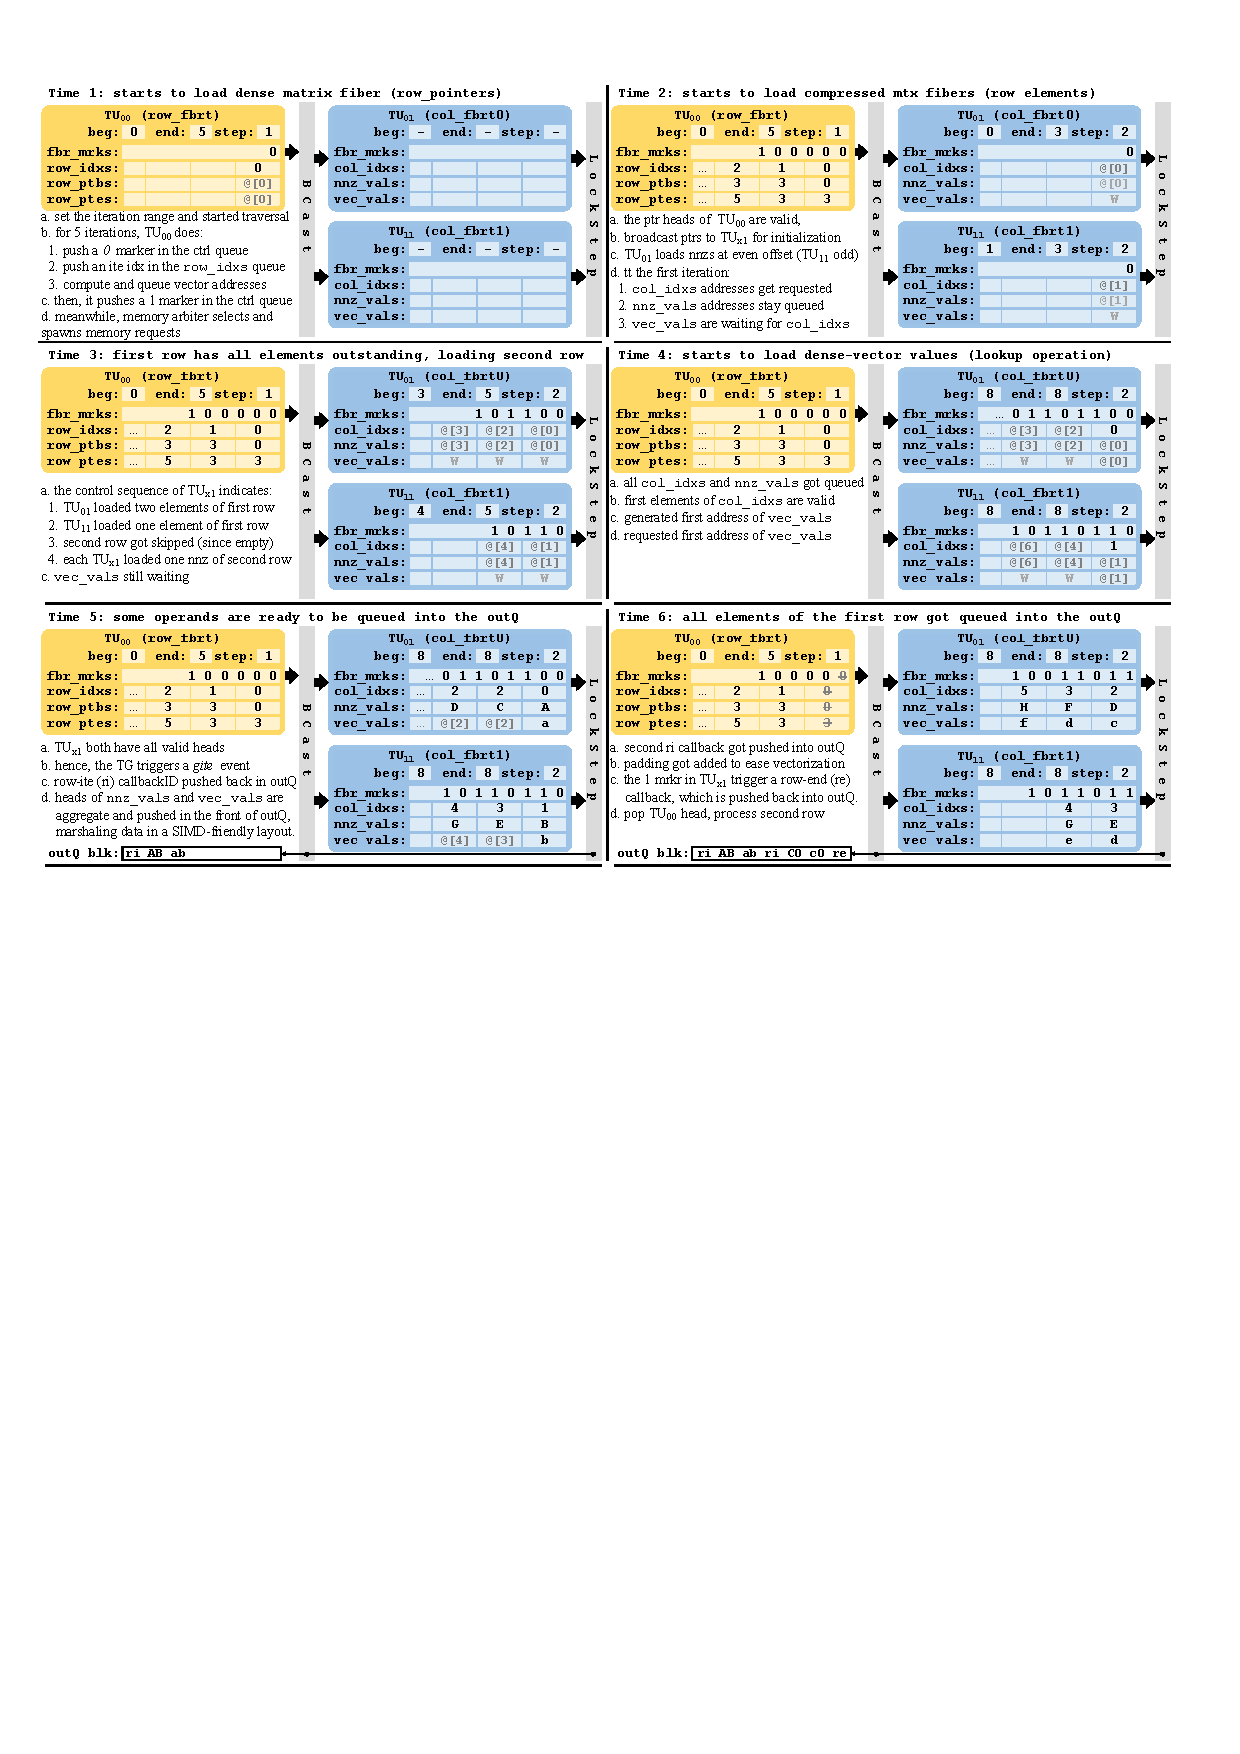
\includegraphics[width=\textwidth,trim=275 260 2 10,clip]{img_spmv_sbs_example.pdf}
        \vspace{-0.5cm}
        \caption{T2: starts to load compressed mtx fibers (row elements)}
        \label{fig:sbs-example-t2}
    \end{subfigure}
    \centering
    \begin{subfigure}[b]{\textwidth}
        \centering
        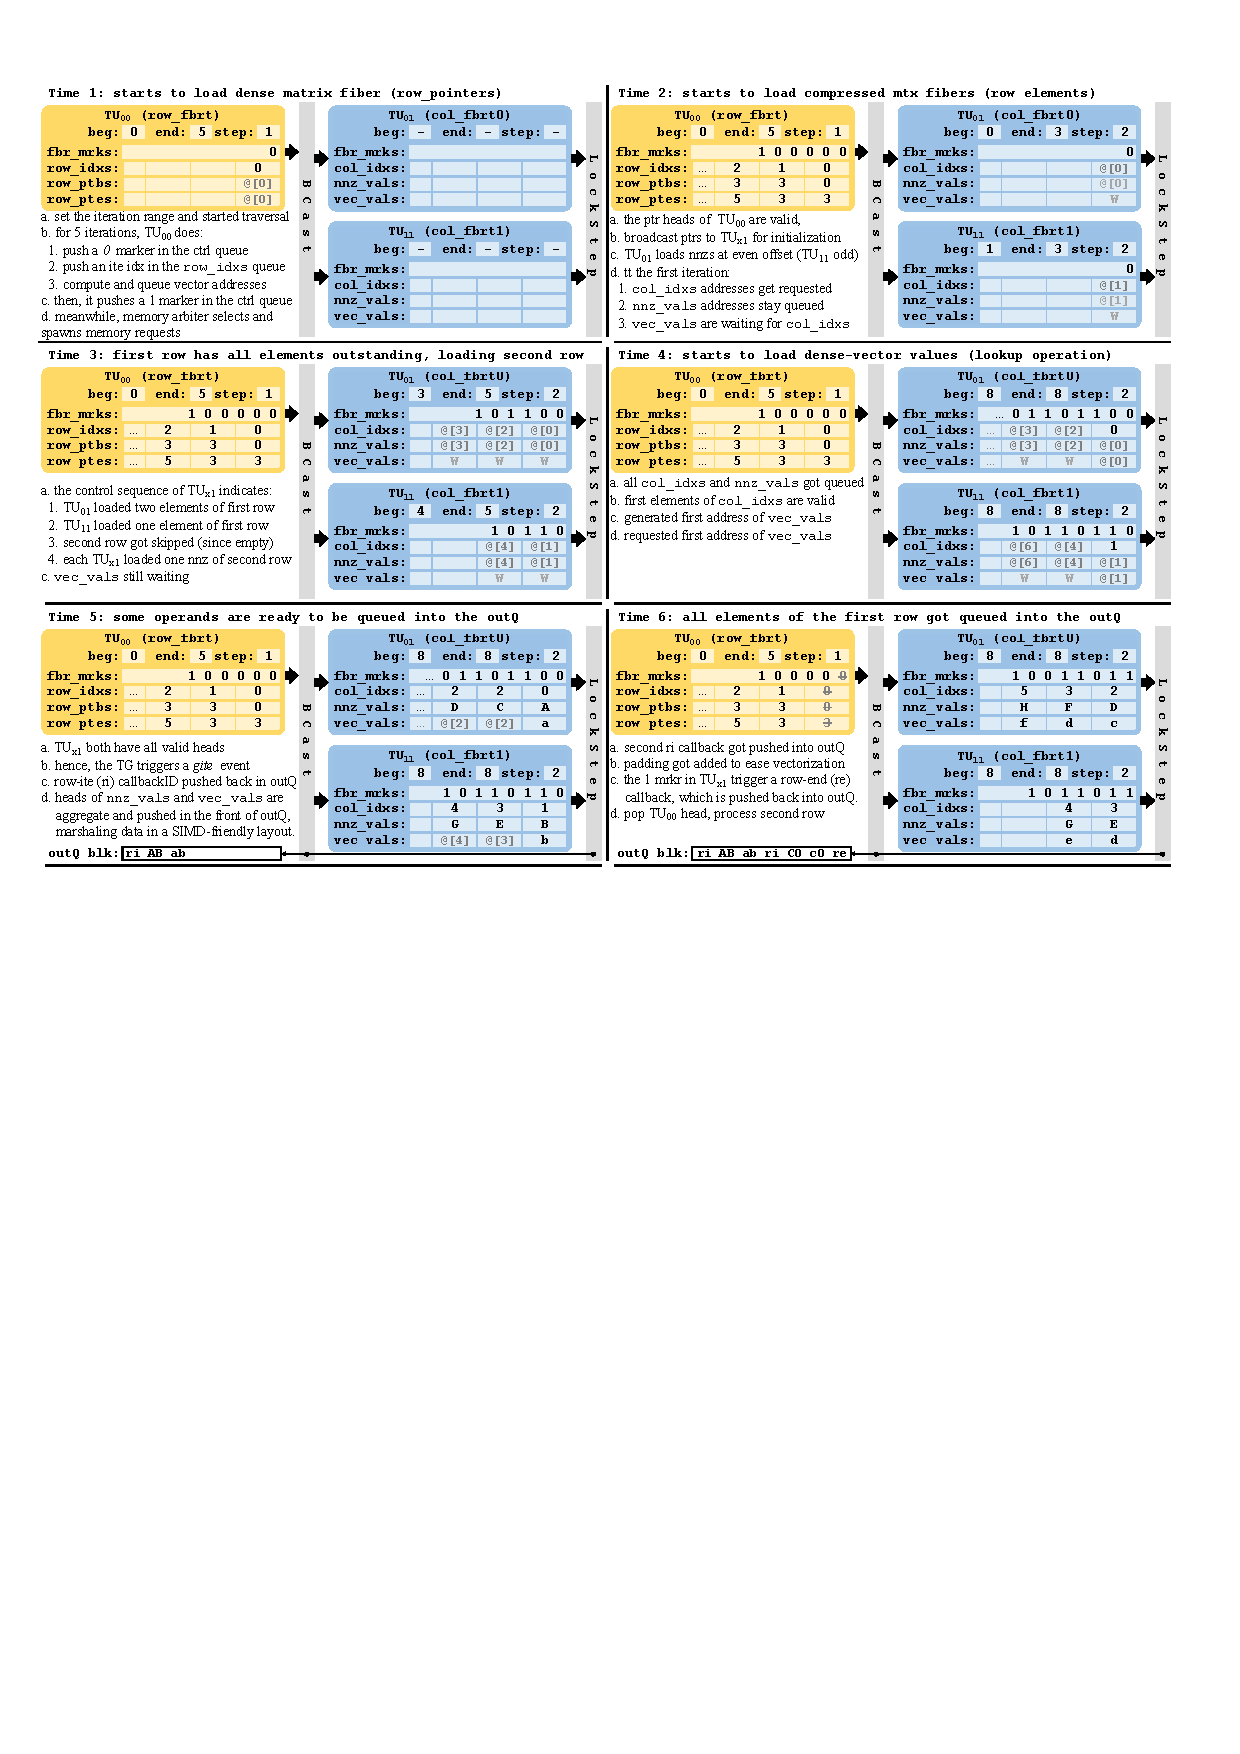
\includegraphics[width=\textwidth,trim=0 130 275 134,clip]{img_spmv_sbs_example.pdf}
        \vspace{-0.5cm}
        \caption{T3: first row has all elements outstanding, loading second row}
        \label{fig:sbs-example-t3}
    \end{subfigure}
    %\vspace{-1em}
  \caption[Step-by-step TMU execution for SpMV, part 1.]{First part of the step-by-step TMU execution of SpMV with inner-loop vectorization (P1 in \Cref{tab:tensor-mapping}) over the CSR matrix in \Cref{fig:sparse-formats}. T1 loads the row-pointer fiber, T2 starts the compressed row traversal, and T3 has issued all requests for the first row while beginning the next row. This shows how the TMU exposes memory-level parallelism before operands are ready for computation.}
  \label{fig:spmv-step-1}
\end{figure}

\begin{figure}
    \centering
    \begin{subfigure}[b]{\textwidth}
        \centering
        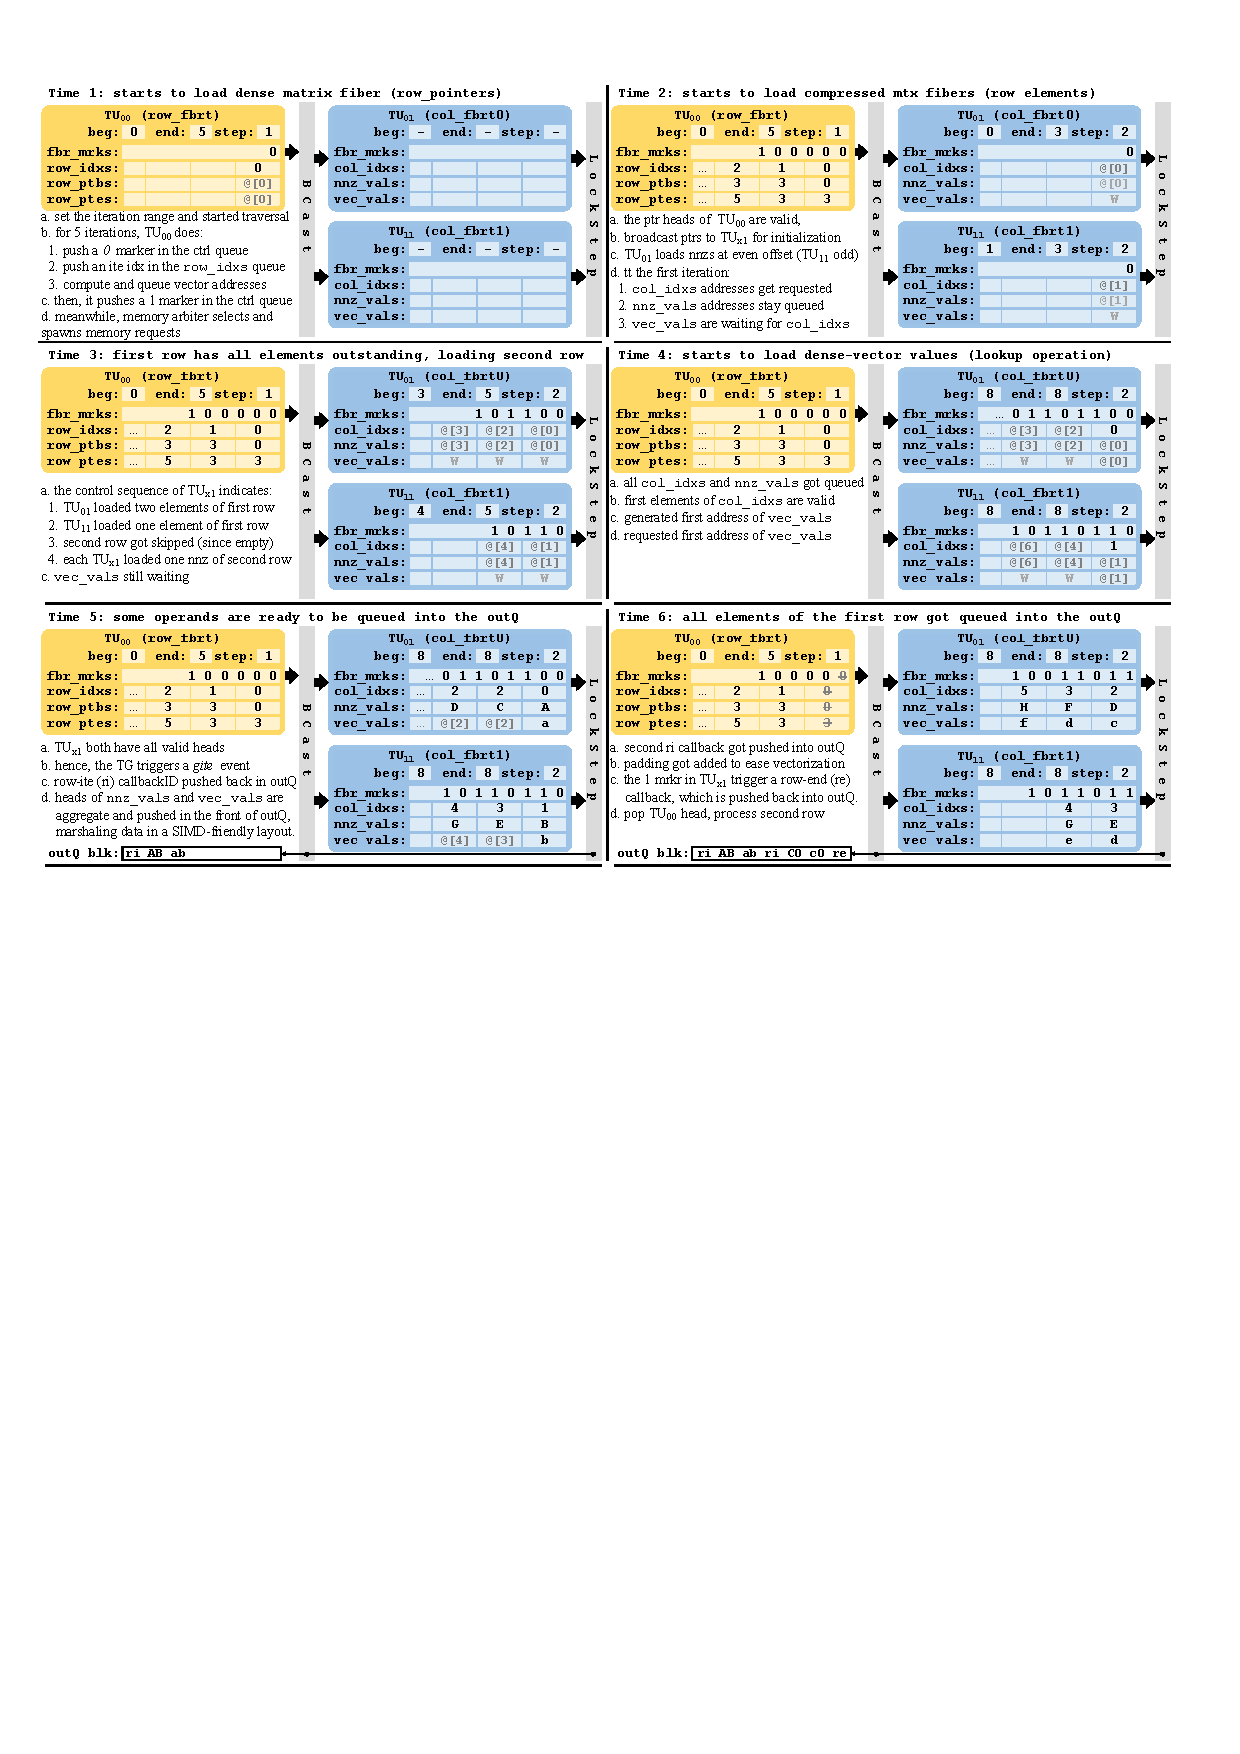
\includegraphics[width=\textwidth,trim=275 130 2 134,clip]{img_spmv_sbs_example.pdf}
        \vspace{-0.5cm}
        \caption{T4: starts to load dense-vector values (lookup operation)}
        \label{fig:sbs-example-t4}
    \end{subfigure}
    \centering
    \begin{subfigure}[b]{\textwidth}
        \centering
        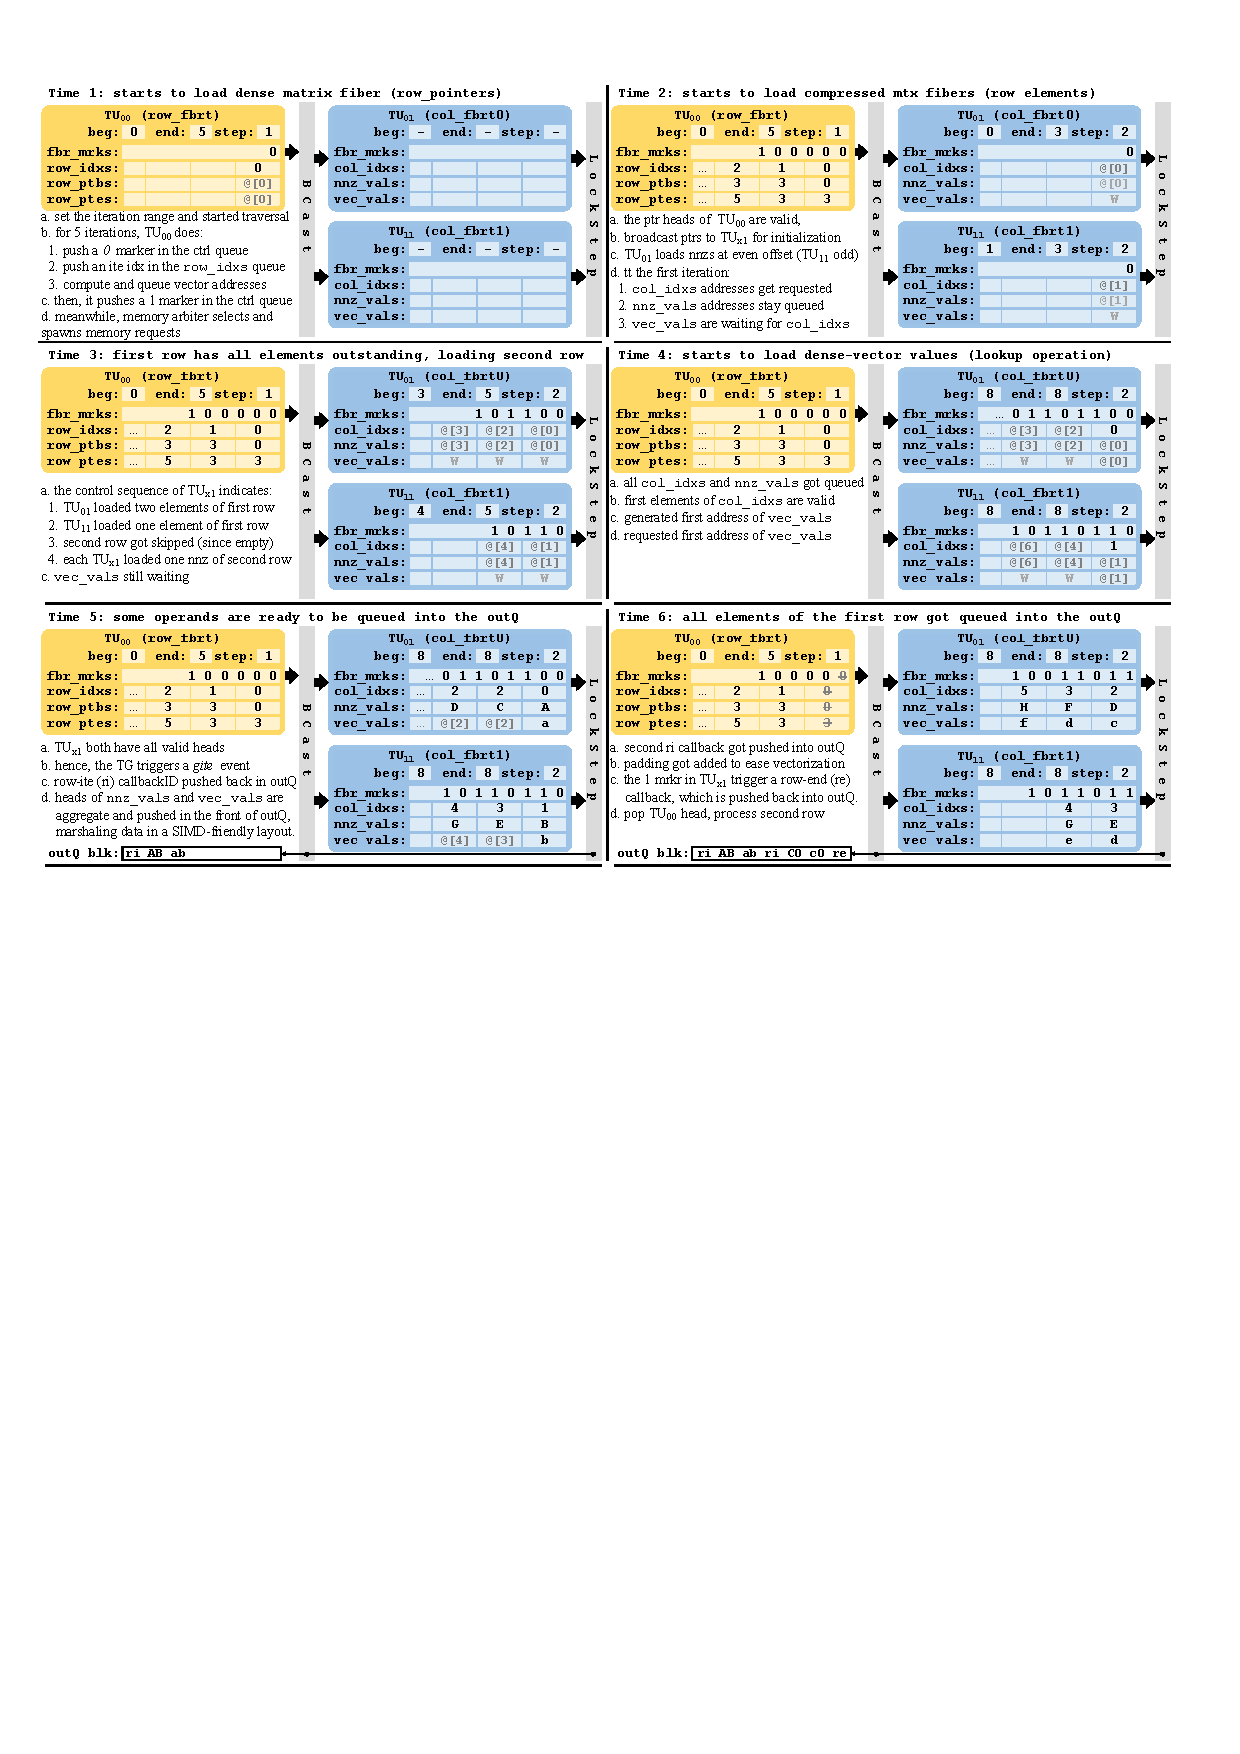
\includegraphics[width=\textwidth,trim=0 4 275 260,clip]{img_spmv_sbs_example.pdf}
        \vspace{-0.5cm}
        \caption{T5: some operands are ready to be queued into the outQ}
        \label{fig:sbs-example-t5}
    \end{subfigure}
    \centering
    \begin{subfigure}[b]{\textwidth}
        \centering
        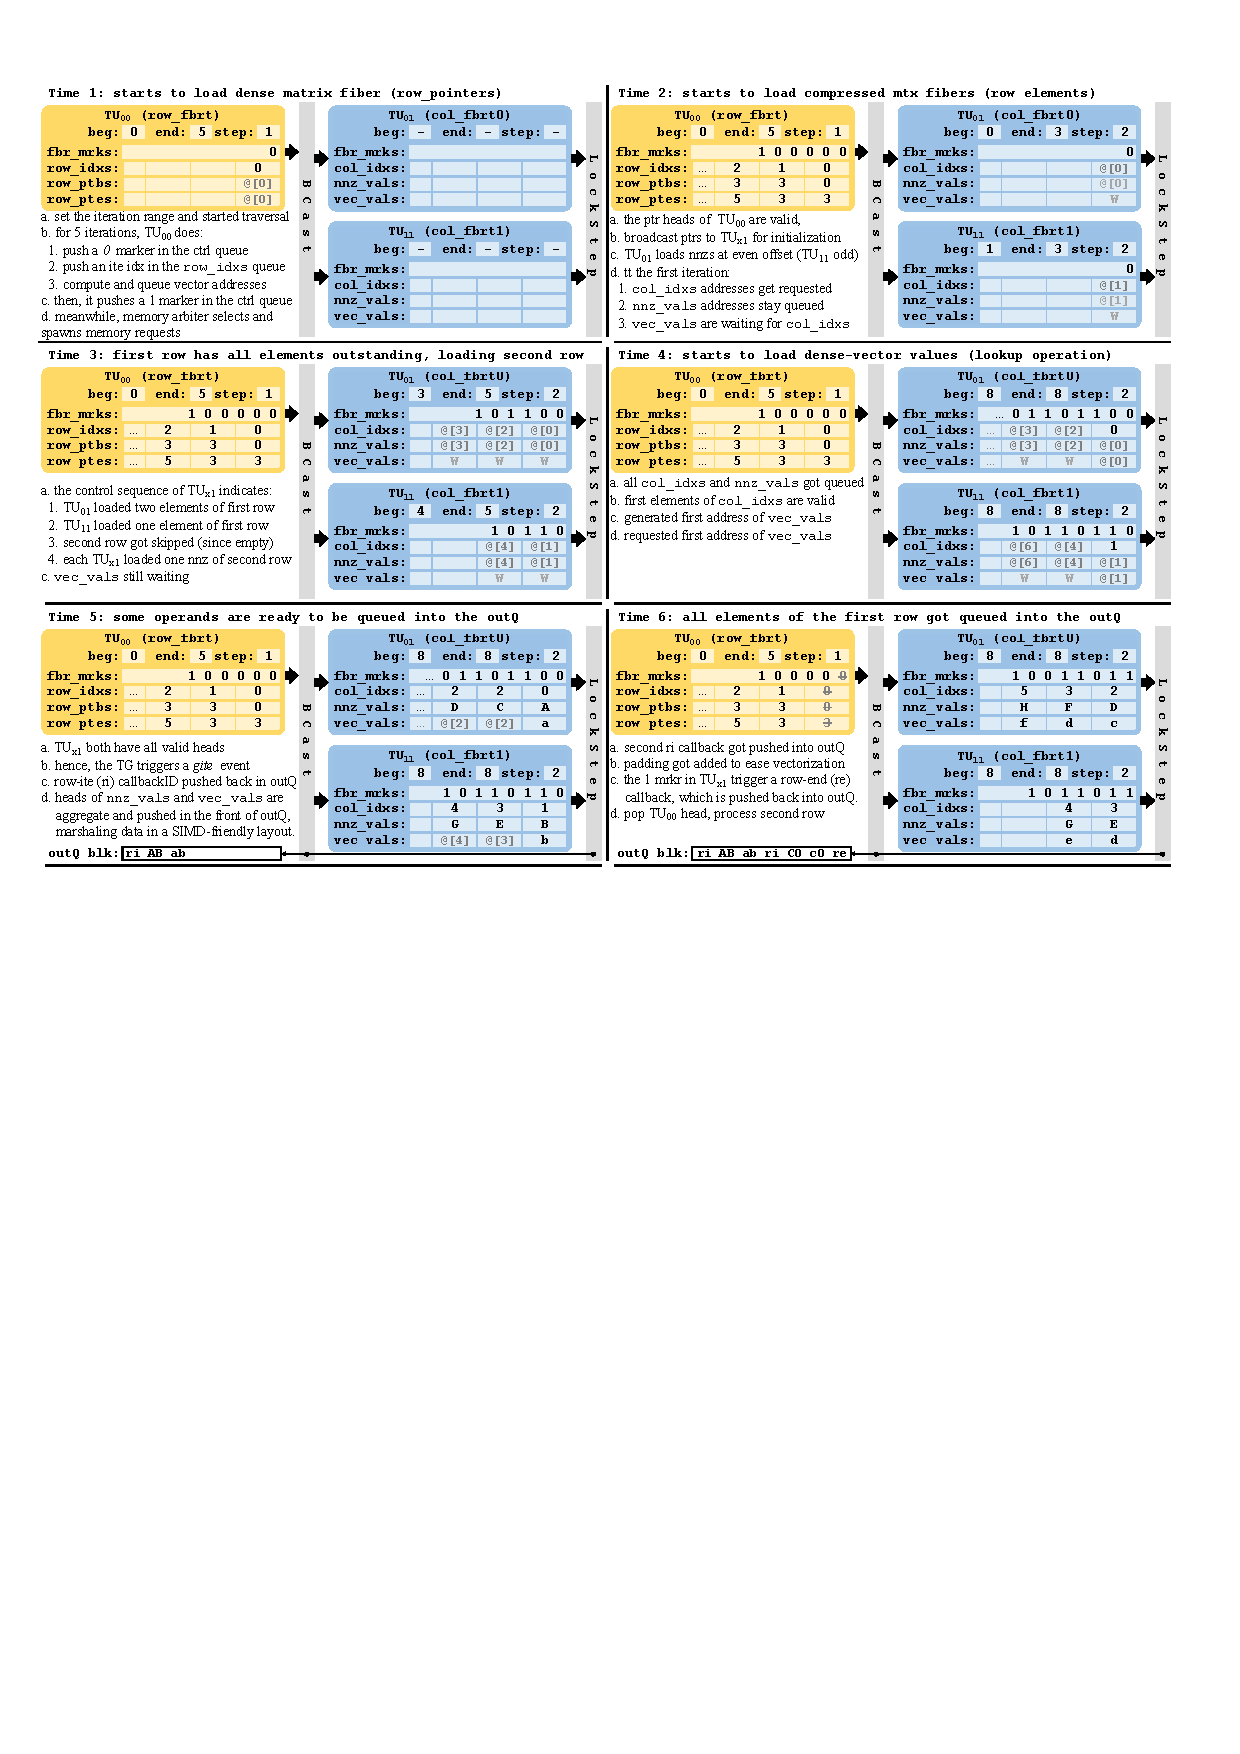
\includegraphics[width=\textwidth,trim=275 4 2 260,clip]{img_spmv_sbs_example.pdf}
        \vspace{-0.5cm}
        \caption{T6: all elements of the first row got queued into the outQ}
        \label{fig:sbs-example-t6}
    \end{subfigure}
    %\vspace{-1em}
  \caption[Step-by-step TMU execution for SpMV, part 2.]{Second part of the step-by-step TMU execution of SpMV with inner-loop vectorization (P1 in \Cref{tab:tensor-mapping}) over the CSR matrix in \Cref{fig:sparse-formats}. T4 issues dense-vector lookups, T5 begins marshaling ready operands into the outQ, and T6 has queued all operands for the first row. This shows how traversal results become ordered callback operands for the core.}
  \label{fig:spmv-step-2}
\end{figure}

%\begin{figure}
%\centering
%  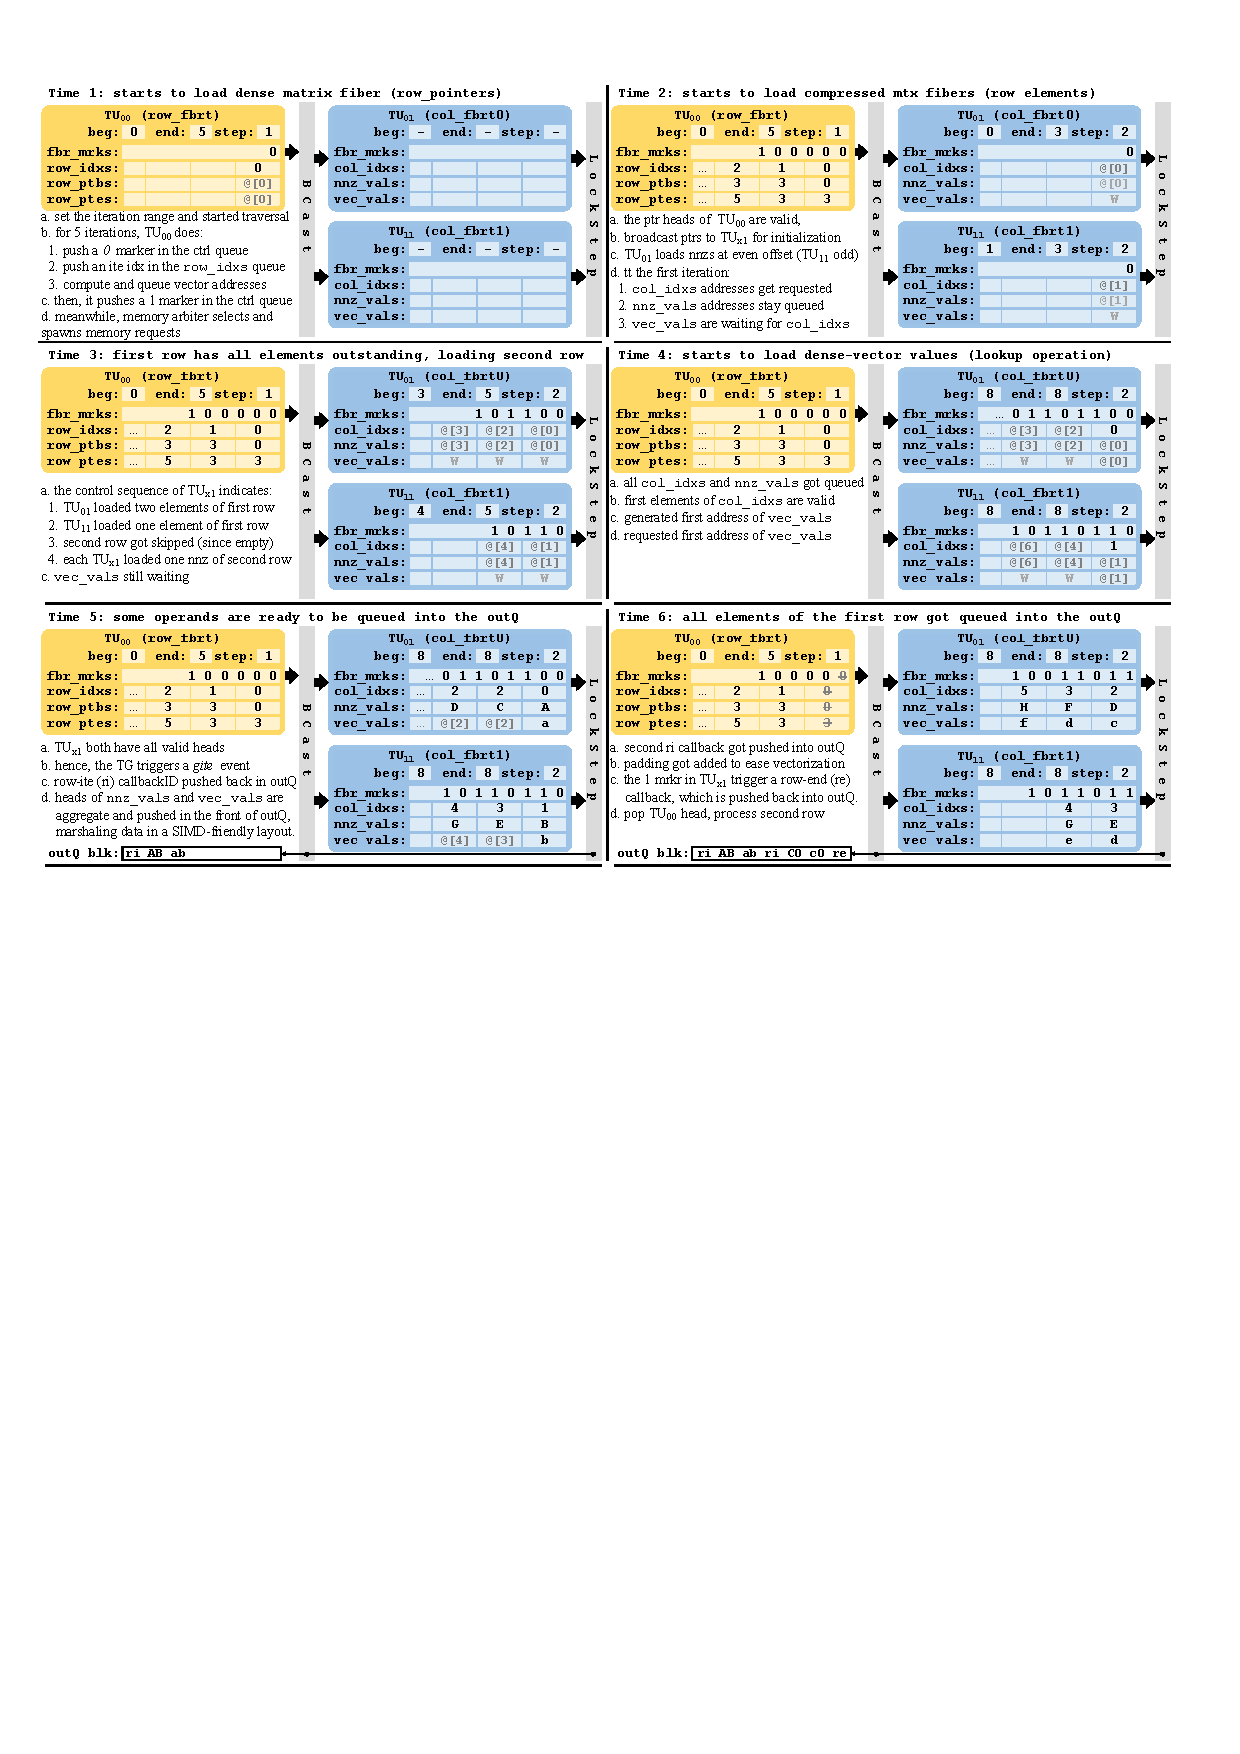
\includegraphics[width=\textwidth]{img_spmv_sbs_example.pdf}
%  \caption{Example performing SpMV with inner-loop vectorization (see \Cref{tab:tmu-data-streams}, P1 version) over the first row of the CSR matrix in %\Cref{fig:sparse-formats}.}
%  \label{fig:spmv_example}
%\end{figure}


In case of conjunctive merging, the \texttt{gite} state (i)~computes the output predicate setting to one of the active lanes with minimum indexes, (ii)~consumes them, and (iii)~pushes a \texttt{0} token into the binary control sequence only if all active lanes have minimum indexes (all-true predicate).
When any active TU has no more elements to merge conjunctively, the \texttt{gend} state pushes a \texttt{1} token into the binary control sequence.

Finally, in case of lockstep co-iteration, the \texttt{gite} state (i) computes the output predicate setting to one of the active lanes not done iterating, (ii) consumes their heads, and (iii) pushes a \texttt{0} token into the binary control sequence.
When all active TUs have no more elements to co-iterate, the \texttt{gend} state pushes a \texttt{1} token into the binary control sequence.

%%%%%%%%%%%%%%%%%%%%%%%%%%%%%%%%%%%%%%%%%%%%%%%%%%%%%%%%%%%%%%%%%%%%%%%%%%%%%%%%%%%%%%%%%%%%%%%%%%%%%%%%%%%%%%%%%%%%%%%%%%%%%%%%%%%
\subsection{Output Queue Construction} \label{sec:output-queue-construction} %%%%%%%%%%%%%%%%%%%%%%%%%%%%%%%%%%%%%%%%%%%%%%%%%%%%%%%%%%%%%%%%%%%%%%%%%%%%%%%%%%%%%%%%%%%%%%%
%%%%%%%%%%%%%%%%%%%%%%%%%%%%%%%%%%%%%%%%%%%%%%%%%%%%%%%%%%%%%%%%%%%%%%%%%%%%%%%%%%%%%%%%%%%%%%%%%%%%%%%%%%%%%%%%%%%%%%%%%%%%%%%%%%%

The predicates and control sequences generated from each TG are then used to push callback IDs and operands into the outQ.
Similarly to traversal and merging, outQ construction is implemented as an FSM running in each TG.
However, while traversal and merging phases can be fully decoupled (i.e., each TU/TG iteration can start as soon as it has valid inputs), outQ generation needs to be serialized across TGs to preserve the order in which callbacks and operands are processed by the core (analogous to out-of-order execution and in-order commit implemented in today's processors).
Hence, besides the \texttt{obeg}, \texttt{oite}, and \texttt{oend} states, outQ  generation also requires \texttt{ow4p} and \texttt{ow4n} states to signal a TG is waiting for the previous or next TG to push data into the outQ.
When a TG is in a \texttt{gbeg}, \texttt{gite}, or \texttt{gend} state, it checks whether there is any callback associated to that state and, if so, it pushes its ID and operands into the outQ buffer.
For performance reasons, both the outQ and outQ buffers are double-buffered.

%%%%%%%%%%%%%%%%%%%%%%%%%%%%%%%%%%%%%%%%%%%%%%%%%%%%%%%%%%%%%%%%%%%%%%%%%%%%%%%%%%%%%%%%%%%%%%%%%%%%%%%%%%%%%%%%%%%%%%%%%%%%%%%%%%%
\subsection{Memory Arbiter} \label{sec:memory-arbiter} %%%%%%%%%%%%%%%%%%%%%%%%%%%%%%%%%%%%%%%%%%%%%%%%%%%%%%%%%%%%%%%%%%%%%%%%%%%%%%%%%%%%%%%%%%%%%%%%%%%%%%%%%%
%%%%%%%%%%%%%%%%%%%%%%%%%%%%%%%%%%%%%%%%%%%%%%%%%%%%%%%%%%%%%%%%%%%%%%%%%%%%%%%%%%%%%%%%%%%%%%%%%%%%%%%%%%%%%%%%%%%%%%%%%%%%%%%%%%%

The TMU sends out memory requests at the cacheline granularity.
For each cycle, the TMU hierarchically selects the next cacheline address to request.
Requests from the leftmost layers (outer loops) are prioritized.
TUs within the same layer are selected round-robin.
Streams within a TU are selected in configuration order.
Requests within the same queue are selected in order.
TUs within the same layer snoop their memory requests and upgrade the status of their \texttt{queued} elements if their address got requested by another TU.

By default, memory requests within a stream are spawned \emph{eager}ly, meaning a cacheline can be requested as soon as an address for that cacheline is computed (\texttt{queued}). In order to reduce memory traffic, certain layers can adopt a \emph{lazy} loading strategy. Lazy loading mode prevents a cacheline to be requested until a different cacheline address is generated within that same queue. This strategy prevents requesting a cacheline multiple times if a queue produces data at a rate lower than the memory latency.

%%%%%%%%%%%%%%%%%%%%%%%%%%%%%%%%%%%%%%%%%%%%%%%%%%%%%%%%%%%%%%%%%%%%%%%%%%%%%%%%%%%%%%%%%%%%%%%%%%%%%%%%%%%%%%%%%%%%%%%%%%%%%%%%%%%
\subsection{TU Queue Sizing} \label{sec:tu-queue-sizing} %%%%%%%%%%%%%%%%%%%%%%%%%%%%%%%%%%%%%%%%%%%%%%%%%%%%%%%%%%%%%%%%%%%%%%%%%%%%%%%%%%%%%%%%%%%%%%%%%%%%%%%%%
%%%%%%%%%%%%%%%%%%%%%%%%%%%%%%%%%%%%%%%%%%%%%%%%%%%%%%%%%%%%%%%%%%%%%%%%%%%%%%%%%%%%%%%%%%%%%%%%%%%%%%%%%%%%%%%%%%%%%%%%%%%%%%%%%%%

All TUs of a layer instantiate, at configuration time, the same amount of streams with the same size. However, since nested loops are mapped from left to right, the rightmost layers load and merge more data than the leftmost ones, leading to different storage requirements. To provide flexibility, all TUs within a lane share the same storage and queues are allocated at configuration time using this shared per-lane storage. This permits shorter queues on leftmost TUs while making full utilization of the available storage, even if some TUs within a lane are not used at all.
Since nested loops are mapped from left to right, the rightmost layers are more utilized than the leftmost ones.
While each TU implements a finite amount of queues with fixed and equal size, we coalesce and multiplex physical layers to meet the performance demand of each logical layer.
Queues are sized with an analytical model which allocates space to layers according to the amount of data to load, which can be statically estimated from the number of nnzs per fiber of the tensor.

%%%%%%%%%%%%%%%%%%%%%%%%%%%%%%%%%%%%%%%%%%%%%%%%%%%%%%%%%%%%%%%%%%%%%%%%%%%%%%%%%%%%%%%%%%%%%%%%%%%%%%%%%%%%%%%%%%%%%%%%%%%%%%%%%%%
\subsection{System Integration} \label{sec:system-integration} %%%%%%%%%%%%%%%%%%%%%%%%%%%%%%%%%%%%%%%%%%%%%%%%%%%%%%%%%%%%%%%%%%%%%%%%%%%%%%%%%%%%%%%%%%%%%%%%%%%%%%
%%%%%%%%%%%%%%%%%%%%%%%%%%%%%%%%%%%%%%%%%%%%%%%%%%%%%%%%%%%%%%%%%%%%%%%%%%%%%%%%%%%%%%%%%%%%%%%%%%%%%%%%%%%%%%%%%%%%%%%%%%%%%%%%%%%

\noindent\textbf{Placement:} 
As shown in \Cref{fig:engine_overview} each core in a multicore system features a TMU. The TMU traverses fibers by loading data from the LLC, and marshals the data into the outQ that is written into the core's private L2 cache. Data from fiber traversals is unlikely to experience reuse from private caches, and by reading from the LLC we take advantage of the larger MSHR count (enabling more MLP). Each outQ is core-private, therefore injecting it into the L2 cache enables faster compute throughput.

\noindent\textbf{Memory subsystem integration:} 
Like prior general-purpose processor engines, the TMU operates with virtual addresses and uses the host core's address translation hardware (MMU)~\cite{spzip2021isca, walkers, AinsworthJ16, hats, yu2015}. In particular, it queries the L2 TLB, and if a page fault occurs, it interrupts the core so the OS can handle the page fault. Once the missing translation is available, the MMU signals the TMU to retry the memory access.

The TMU operates decoupled from the host core, issuing coherent read-only memory requests (fiber traversals) that do not affect coherence or consistency. TMU produces the outQ that is written (write-only) into the private L2 cache of the host core. While the outQ data may be evicted into shared cache levels, this data is not shared across cores. Therefore, there is no shared read-write data between the TMU and the host core or other cores in the system.

\noindent\textbf{Context switching and exceptions:}
TMU architectural state must be saved and restored when a thread is context-switched. When the OS deschedules a thread that uses the TMU, it quiesces the TMU, saves its context, and restores it when the thread is rescheduled. 
On exceptions or syscalls, this is not necessary, as the TMU is not used by the OS; similarly, the FPU state is not saved.
The minimum context state that needs to be saved is the initial TMU configuration (e.g., queue types and sizes, \texttt{beg} and \texttt{end} iteration boundaries), the head of each TU \texttt{ite} stream, and some control registers such as the base outQ address and current writing offset. The memory-mapped outQ is private per thread.
Fortunately, support to efficiently save large state is already implemented in the Linux kernel via on-demand expansion of per-task context switch buffers. This is used by the new Intel Advanced Matrix eXtensions (AMX)~\cite{amx}, which employ tile registers that already occupy 8KB in current implementations.

%%%%%%%%%%%%%%%%%%%%%%%%%%%%%%%%%%%%%%%%%%%%%%%%%%%%%%%%%%%%%%%%%%%%%%%%%%%%%%%%%%%%%%%%%%%%%%%%%%%%%%%%%%%%%%%%%%%%%%%%%%%%%%%%%%%
\subsection{Step-by-Step Example} \label{sec:step-by-step-example} %%%%%%%%%%%%%%%%%%%%%%%%%%%%%%%%%%%%%%%%%%%%%%%%%%%%%%%%%%%%%%%%%%%%%%%%%%%%%%%%%%%%%%%%%%%%%%%%%%%%
%%%%%%%%%%%%%%%%%%%%%%%%%%%%%%%%%%%%%%%%%%%%%%%%%%%%%%%%%%%%%%%%%%%%%%%%%%%%%%%%%%%%%%%%%%%%%%%%%%%%%%%%%%%%%%%%%%%%%%%%%%%%%%%%%%%

\Cref{fig:spmv_example_1} and \ref{fig:spmv_example_2} picture a step-by-step example for SpMV (\Cref{fig:spmv_decomposition}) where the TMU has been programmed using the code in \Cref{fig:spmv_programmability}. The example loads the CSR matrix shown in \Cref{fig:sparse_formats} and assumes a two-lane design.

The reminder of this chapter demonstrates the performance potential of the TMU for accelerating sparse tensor algebra kernels in scientific and machine learning models.

%%%%%%%%%%%%%%%%%%%%%%%%%%%%%%%%%%%%%%%%%%%%%%%%%%%%%%%%%%%%%%%%%%%%%%%%%%%%%%%%%%%%%%%%%%%%%%%%%%%%%%%%%%%%%%%%%%%%%%%%%%%%%%%%%%%
\section{The Potential of Accelerating Scientific Computation with the TMU} \label{sec:dae-potential-scientific} %%%%%%%%%%%%%%
%%%%%%%%%%%%%%%%%%%%%%%%%%%%%%%%%%%%%%%%%%%%%%%%%%%%%%%%%%%%%%%%%%%%%%%%%%%%%%%%%%%%%%%%%%%%%%%%%%%%%%%%%%%%%%%%%%%%%%%%%%%%%%%%%%%
In this section we first evaluate TMU performance on scientificc sparse tensor algebra kernels with respect to traditional architectures. Then, we provide a sensitivity analysis on TMU storage and SVE vector length. Finally, we compare the TMU to existing scalar engines. Next section evaluates the TMU in accelerating machine learning models.

%%%%%%%%%%%%%%%%%%%%%%%%%%%%%%%%%%%%%%%%%%%%%%%%%%%%%%%%%%%%%%%%%%%%%%%%%%%%%%%%%%%%%%%%%%%%%%%%%%%%%%%%%%%%%%%%%%%%%%%%%%%%%%%%%%%
\subsection{Experimental Methodology} \label{sec:experimental-methodology-sparse} %%%%%%%%%%%%%%%%%%%%%%%%%%%%%%%%%%%%%%%%%%%%%%%%%%%%%%%%%%%%%%%%
%%%%%%%%%%%%%%%%%%%%%%%%%%%%%%%%%%%%%%%%%%%%%%%%%%%%%%%%%%%%%%%%%%%%%%%%%%%%%%%%%%%%%%%%%%%%%%%%%%%%%%%%%%%%%%%%%%%%%%%%%%%%%%%%%%%

%%%%%%%%%%%%%%%%%%%%%%%%%%%%%%%%%%%%%%%%%%%%%%%%%%%%%%%%%%%%%%%%%%%%%%%%%%%%%%%%%%%%%%%%%%%%%%%%%%%%%%%%%%%%%%%%%%%%%%%%%%%%%%%%%%%
\subsubsection{Simulation Infrastructure:} \label{sec:simulation-infrastructure-sparse} %%%%%%%%%%%%%%%%%%%%%%%%%%%%%%%%%%%%%%%%%%%%%%%%%%%%%%%%%%%%%%%%%%%%%%%%%%%%%%%%%%%%%%%%%%%
%%%%%%%%%%%%%%%%%%%%%%%%%%%%%%%%%%%%%%%%%%%%%%%%%%%%%%%%%%%%%%%%%%%%%%%%%%%%%%%%%%%%%%%%%%%%%%%%%%%%%%%%%%%%%%%%%%%%%%%%%%%%%%%%%%%

\begin{table}
\centering
\caption[Specifications of the simulated DAE multicore for scientific workloads.]{Specifications of the simulated DAE multicore processor used for the scientific sparse-tensor evaluation. The DAE system combines high-performance DAE cores each composed of a TMU and an Arm-like core, an HBM-backed memory hierarchy, and a mesh interconnect. The TMU and LLC capacities are balanced at the system level: the sum of outstanding-request slots across TMUs matches the sum of MSHRs across LLC slices.}
    \begin{tabular}{@{}ll@{}}
    \toprule
    \textbf{Cores} & 8 Neoverse-N1-like out-of-order cores at 2.4GHz\\
    \textbf{SVE width} & 512 bits \\
    \textbf{Reorder buffer} & 224 entries \\
    \textbf{Load/Store queues} & 96 entries, 96 entries \\
    \midrule
    \textbf{Private L1 I\&D} & 64 KiB/core, 4-way, 2 cycle data access, 32 MSHRs \\
    \textbf{L1I prefetcher} & Tagged \\
    \textbf{L1D prefetcher} & Stride, degree 2 \\
    \textbf{Private L2}     & 512 KiB/core, 8-way, 8 cycle data access, 64 MSHRs \\
    \textbf{L2 prefetcher}  & Best Offset Prefetcher \\
    \textbf{Shared L3 (LLC)} & Mostly exclusive, 8 slices of 1MiB, 16 ways, \\
       & 12 cycles data access, 128 MSHRs \\
    \midrule
    \textbf{Coherence protocol} & MOESI-like AMBA 5 CHI specification \\% without DCT \& DMT \\
    \textbf{Network topology} & $4\times4$ 2D mesh, 1 cycle routers, 1 cycle links\\
    \midrule
    \textbf{Memory} & 4 HBM2e channels, FR-FCFS, 37.5GB/s per channel\\
    \midrule
    \textbf{TMU} & 2KB per-lane storage, 8 lanes, 4 TGs with mergers\\
        & 128 outstanding requests \\    
    \bottomrule
    \end{tabular}
\label{tab:tmu-dae-system-specs}
\end{table}


We evaluate the TMU using the gem5 v20.1.0.0 simulator~\cite{lowepower2020gem5}. We simulate a multicore system consisting of 8 Neoverse-N1-like out-of-order cores, three levels of cache, 4 HBM2e memory channels, and a mesh-based network-on-chip modeling the AMBA 5 CHI protocol. Each core features a TMU engine that faithfully models the described architecture. The simulated system runs Ubuntu 20.04 with Linux kernel 5.4.65. \Cref{table:gem5} summarizes the architectural parameters.

%%%%%%%%%%%%%%%%%%%%%%%%%%%%%%%%%%%%%%%%%%%%%%%%%%%%%%%%%%%%%%%%%%%%%%%%%%%%%%%%%%%%%%%%%%%%%%%%%%%%%%%%%%%%%%%%%%%%%%%%%%%%%%%%%%%
\subsubsection{Workloads:} %%%%%%%%%%%%%%%%%%%%%%%%%%%%%%%%%%%%%%%%%%%%%%%%%%%%%%%%%%%%%%%%%%%%%%%%%%%%%%%%%%%%%%%%%%%%%%%%%%%%%%%%%%%
%%%%%%%%%%%%%%%%%%%%%%%%%%%%%%%%%%%%%%%%%%%%%%%%%%%%%%%%%%%%%%%%%%%%%%%%%%%%%%%%%%%%%%%%%%%%%%%%%%%%%%%%%%%%%%%%%%%%%%%%%%%%%%%%%%%
\begin{table}
\centering
\caption[Selected inputs for scientific sparse tensor workloads.]{Inputs for the scientific sparse tensor workloads. The table lists SuiteSparse matrices for sparse linear algebra kernels and FROSTT tensors for sparse tensor kernels, along with nonzero counts, dimensions, domains, and matrix-structure visualizations. These inputs span different sparsity patterns and domains, stressing traversal, lookup, and merging in different ways.}
\label{tab:tmu-scientific-inputs}
\resizebox{\columnwidth}{!}{%
\begin{tabular}{@{}cccccc@{}}
\toprule
\textbf{Id} & \textbf{Matrix~\cite{davis2011university}} & \textbf{nnzs} & \textbf{rows} & \textbf{nnzs/row} & \textbf{Domain}\\
\midrule
M1 & af\_0\_k101 & 17.6M & 504K & $\sim$35 & structural  \\
M2 & atmosmodm & 10.3M & 1.5M & $\sim$7     & fluid dynamic  \\
M3 & Freescale1 & 17.1M & 3.4M & $\sim$5    & circuit simulation \\
M4 & gb\_osm & 13.3M & 7.7M & $\sim$2   & graph  \\
M5 & halfb & 12.4M & 225K & $\sim$55         & structural  \\
M6 & test1 & 9.4M & 393K & $\sim$24          & semiconductor  \\
\hline
\textbf{Id} & \textbf{Tensor~\cite{smith2017frostt}} & \textbf{nnzs} & \multicolumn{2}{c}{\textbf{Dimensions}} & \textbf{Domain} \\
\hline
T1 & Chicago-crime & 5M & \multicolumn{2}{c}{6K x 24 x 77 x 32} & count\\
T2 & LBNL-network & 2M & \multicolumn{2}{c}{2K x 4K x 2K x 4K x 1M} & network \\
T3 & NIPS pubs & 3M & \multicolumn{2}{c}{3K x 3K x 14K x 17} & text \\
T4 & Uber pickups & 3M & \multicolumn{2}{c}{183 x 24 x 1K x 2K} & map\\
\hline
\textbf{M1} & \textbf{M2} & \textbf{M3} & \textbf{M4} & \textbf{M5} & \textbf{M6} \\ 
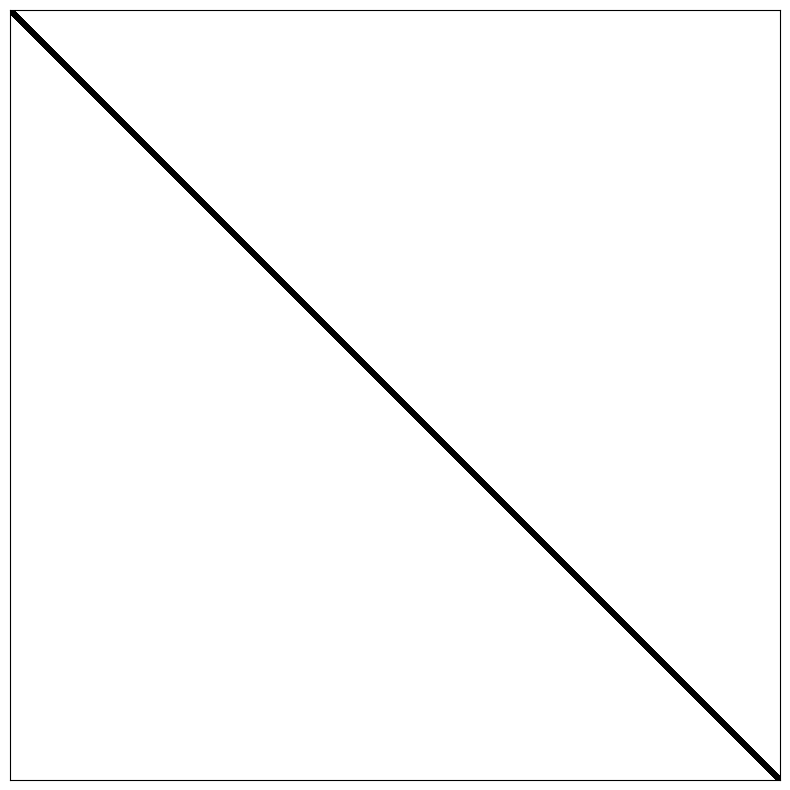
\includegraphics[width=.2\linewidth]{img_mtx_af_0_k101-crop.png}  &
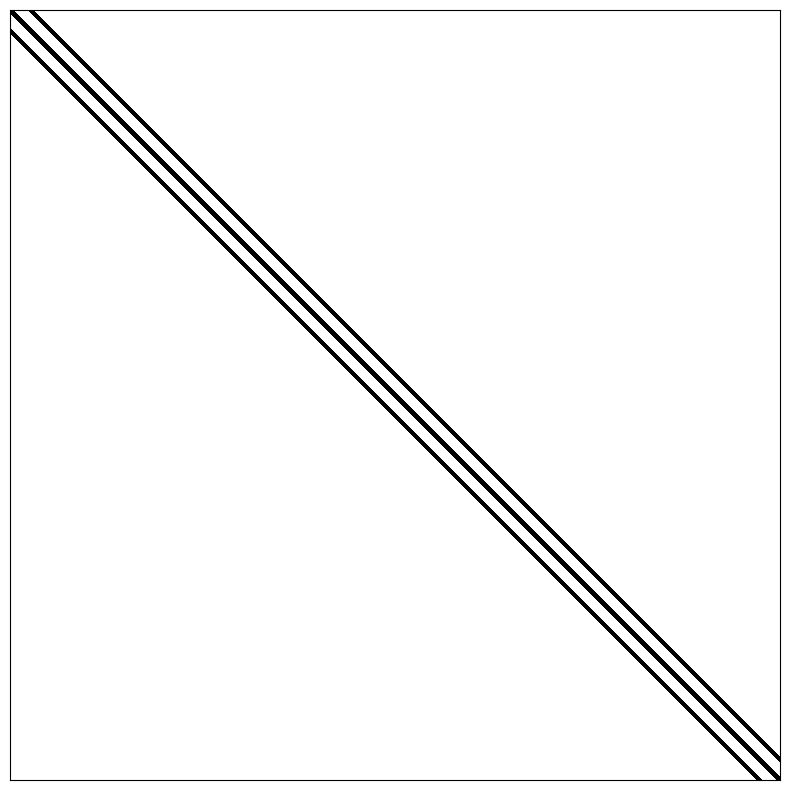
\includegraphics[width=.2\linewidth]{img_mtx_atmosmodm-crop.png}  &
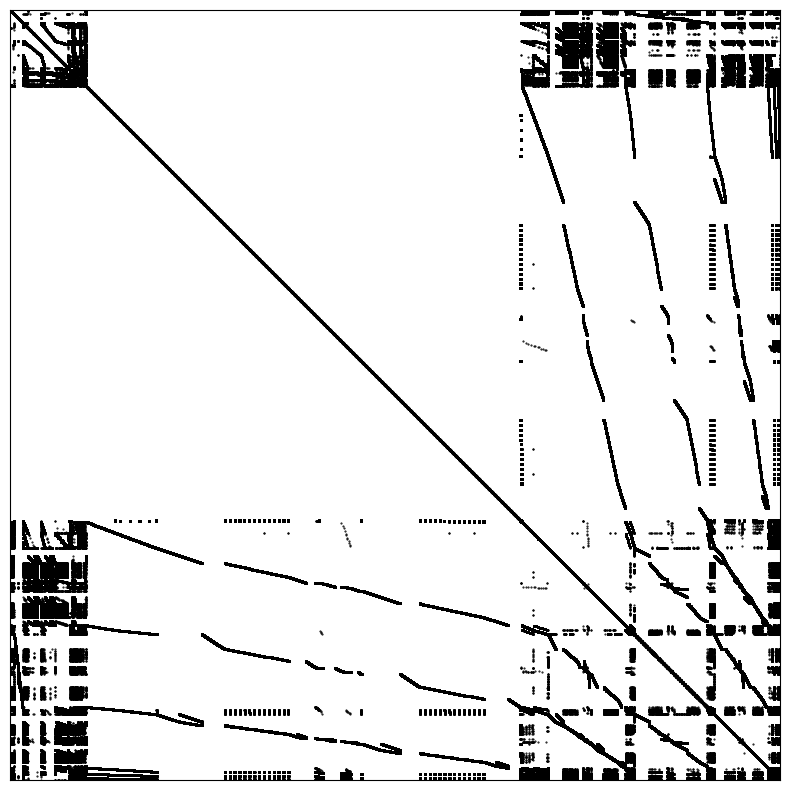
\includegraphics[width=.2\linewidth]{img_mtx_Freescale1-crop.png}  &
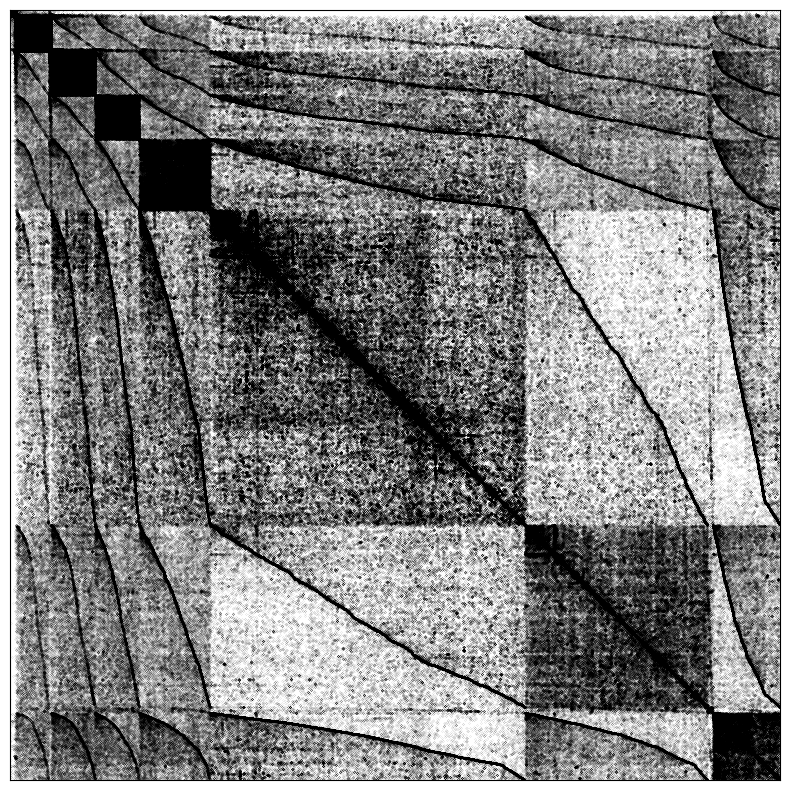
\includegraphics[width=.2\linewidth]{img_mtx_great-britain_osm-crop.png}  &
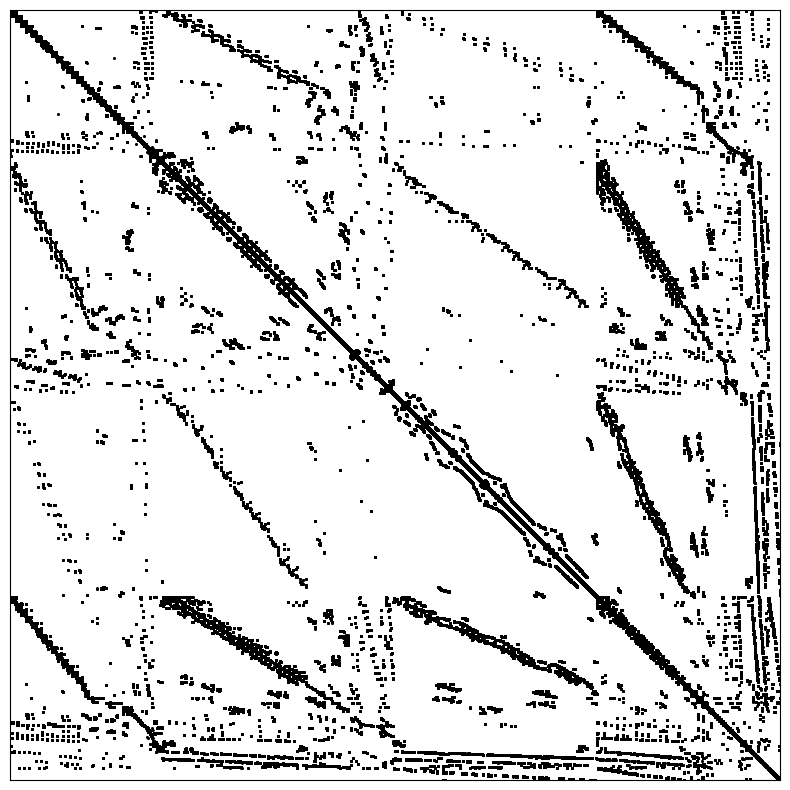
\includegraphics[width=.2\linewidth]{img_mtx_halfb-crop.png}  &
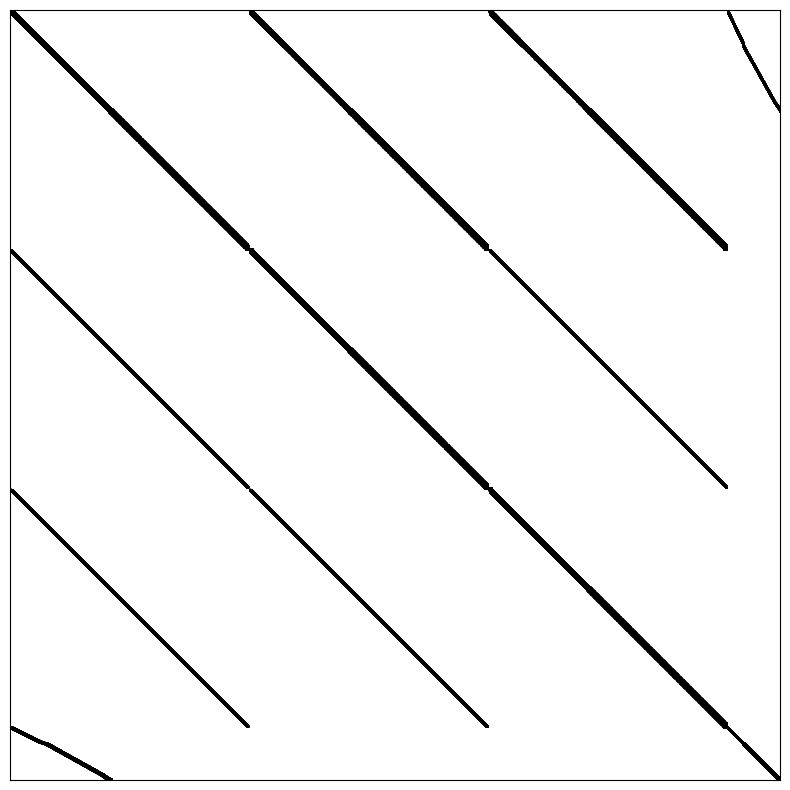
\includegraphics[width=.2\linewidth]{img_mtx_test1-crop.png} \\
\bottomrule
\end{tabular}
}
\end{table}

We evaluate our proposal over several sparse linear and tensor algebra kernels and real-world applications with different characteristics. We employ high-performance multi-threaded software baselines which we either generated by the well-known TACO compiler~\cite{taco2017oopsla} or extracted from existing reference libraries~\cite{phipps2019genten,liu2021sparta}.
We vectorized all baselines with Arm SVE and utilized vector gather and scatter instructions where appropriate.
In particular, we evaluate the following kernels from \Cref{tab:tensor-mapping}:
\begin{itemize}
    \item \textbf{SpMV CSR}~\cite{williams2007spmv}: Software baseline from TACO vectorized with Arm SVE. The TMU implements inner-loop vectorization (P1). 
    \item \textbf{SpMSpM CSR}~\cite{gao2023spgemm_survey}: Implements $Z=AA^T$. Software baseline from TACO vectorized with Arm SVE. The TMU implements inner-loop vectorization (P2).
    \item \textbf{SpKAdd DCSR}~\cite{hussain2022spkadd}: Software baseline from TACO (\textit{k}=8) vectorized with Arm SVE. To preserve domain characteristics, input matrices ($A^x$ with $x=1...k$) are generated by cyclically distributing rows of the original matrix ($A$) to each input matrix (i.e., \textit{i}-th row of input $A^x_i=A_{i*k+x}$).
    \item \textbf{MTTKRP COO}~\cite{phipps2019genten}: Performs a Matricized COO Tensor Times Khatri-Rao Product with the permutation optimization proposed by Phipps et al.~\cite{phipps2019genten}. The TMU implements parallelism at the mode (P1) and rank (P2) levels.
    \item \textbf{SpTC CSF}~\cite{liu2021sparta}: Performs a tensor contraction of two CSF tensors with the expressions evaluated by Liu et al.~\cite{liu2021sparta}. We evaluate the symbolic phase to limit simulation time.
\end{itemize}
Moreover, we evaluate the following real-world applications:
\begin{itemize}
    \item \textbf{PR}: Performs the PageRank algorithm as implemented in the GAP Benchmark suite~\cite{beamer2015gapbs} (Jacobi-style method), optimized with Arm SVE.
    \item \textbf{TC}: Counts the triangles in a graph as in the fused GraphBLAS version~\cite{graphblascppspec} based on masked SpMSpM~\cite{milanovic2022masked}.
    \item \textbf{CP-ALS}~\cite{phipps2019genten}: Performs a canonical polyadic decomposition of a COO tensor with an alternating least squares algorithm, from the GenTen framework~\cite{phipps2019genten}.
\end{itemize}
We run these applications with the settings suggested by the authors.
\Cref{tab:inputs} describes the inputs we used for all linear and tensor algebra applications, from SuiteSparse~\cite{suitesparse2011acm} and FROSTT~\cite{frosttdataset}, respectively.

%%%%%%%%%%%%%%%%%%%%%%%%%%%%%%%%%%%%%%%%%%%%%%%%%%%%%%%%%%%%%%%%%%%%%%%%%%%%%%%%%%%%%%%%%%%%%%%%%%%%%%%%%%%%%%%%%%%%%%%%%%%%%%%%%%%
\subsection{Performance Analysis} %%%%%%%%%%%%%%%%%%%%%%%%%%%%%%%%%%%%%%%%%%%%%%%%%%%%%%%%%%%%%%%%%%%%%%%%%%%%%%%%%%%%%%%%%%%%%%%%%
%%%%%%%%%%%%%%%%%%%%%%%%%%%%%%%%%%%%%%%%%%%%%%%%%%%%%%%%%%%%%%%%%%%%%%%%%%%%%%%%%%%%%%%%%%%%%%%%%%%%%%%%%%%%%%%%%%%%%%%%%%%%%%%%%%%

\begin{figure}
    \centering
    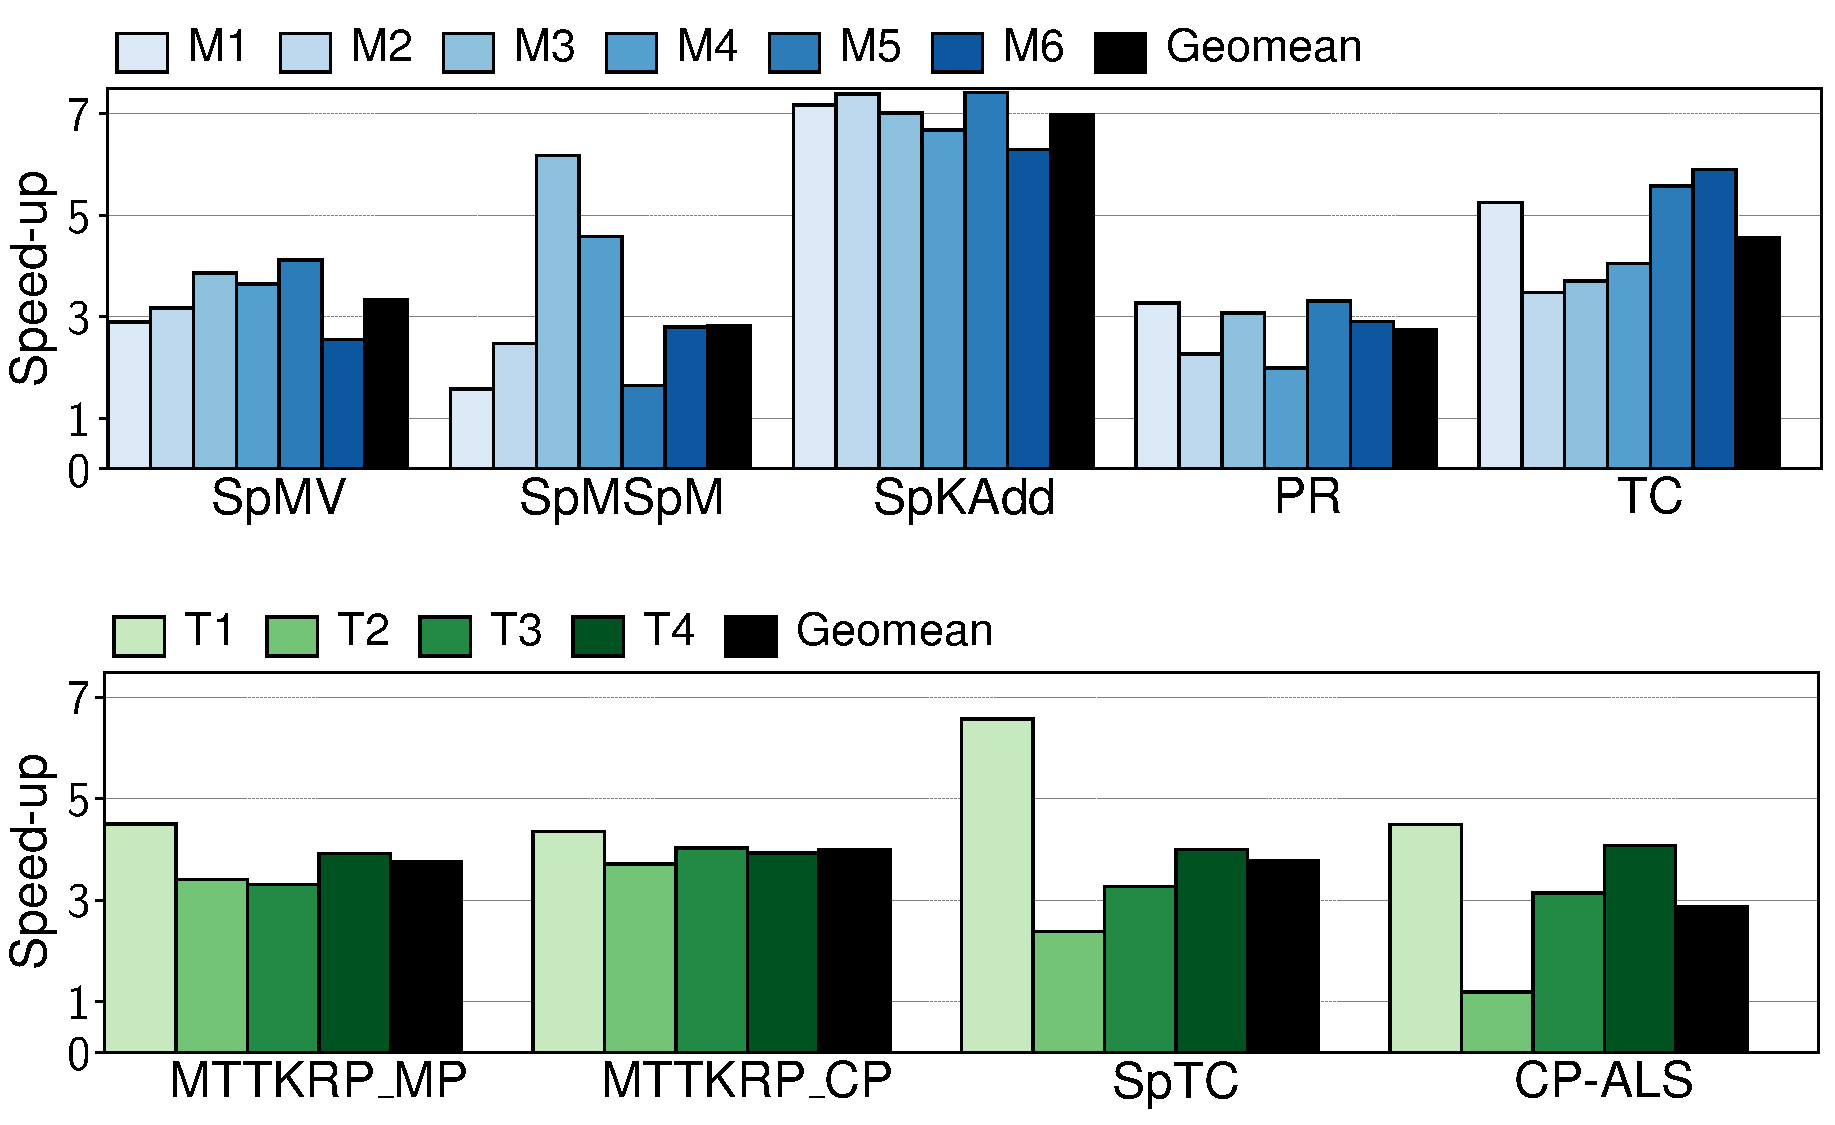
\includegraphics[width=0.8\textwidth]{img_speed_ups_16_stacked.pdf}
    \caption[TMU speedups for scientific kernels.]{TMU speedups for linear (top) and tensor (bottom) algebra workloads with respect to baseline. Bars are different matrices.}
    \label{fig:speedups_lin_tns_alg_wrt_sw}
\end{figure}

\begin{figure}
    \centering
    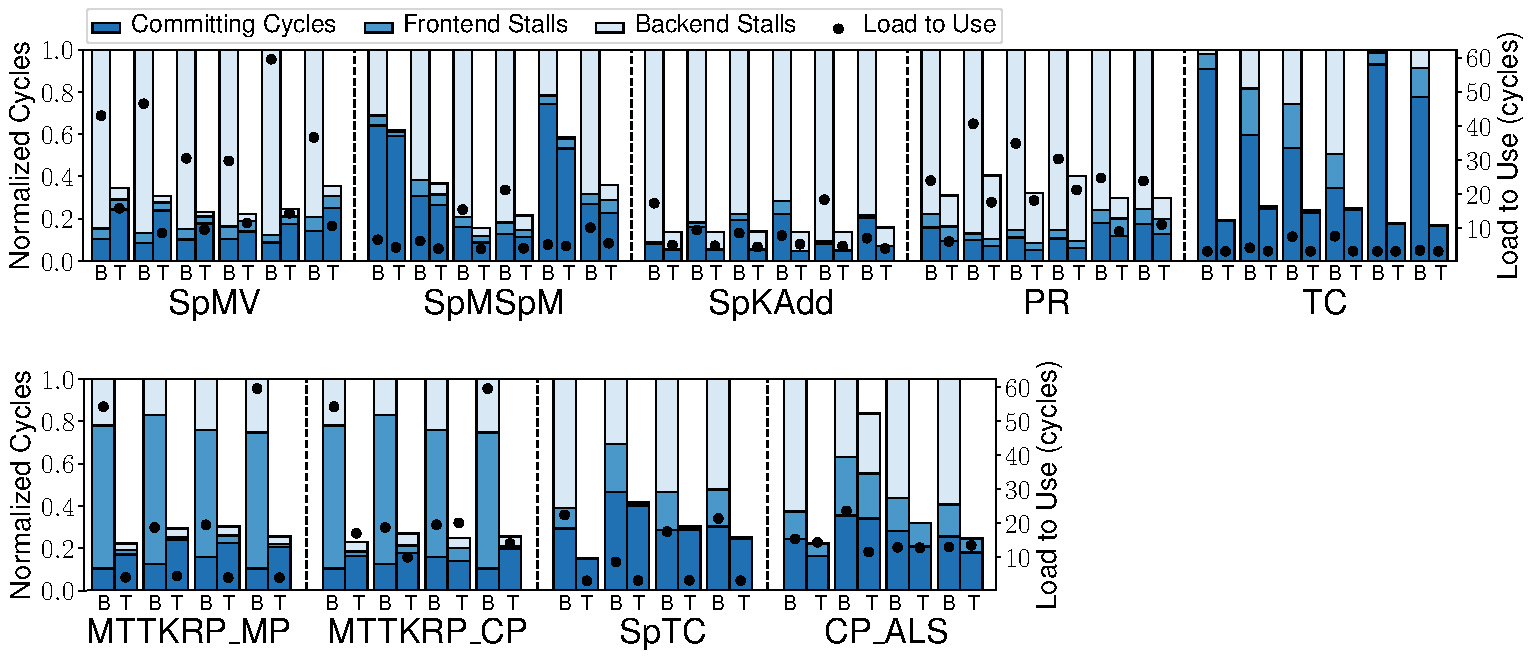
\includegraphics[width=\textwidth]{img_breakdown_frontend_stacked.pdf}
    \caption[Performance breakdown of a CPU and DAE processor on scientific kernels.]{Normalized cycles breakdown for traditional processors and DAE processors. Groups of bars are different kernels. Pairs of bars are different inputs. The leftmost bar in the pair indicates TMU (T) whereas the rightmost indicates baseline (B). Each bar shows (i) committing cycles, (ii) frontend stalls, and (iii) backend stalls. Dots indicate average load-to-use latency (right y-axis). }
    \label{fig:breakdown}
\end{figure}

\Cref{fig:speedups_lin_tns_alg_wrt_sw} reports the performance speedups achieved by the TMU over the software baselines detailed in \Cref{sec:experimental-methodology-sparse}. Overall, the proposed system achieves geomean performance speedups of 3.58$\times$, 2.82$\times$, and 4.94$\times$ on memory-intensive (SpMV, PR, MTTKRP, CP-ALS), compute-intensive (SpMSpM), and merge-intensive (SpKAdd, TC, SpTC) workloads, respectively. %, and an average Xx performance speedup on real-world applications. 
\Cref{fig:breakdown} shows, for each evaluated workload and input, the normalized cycles spent (left y-axis) (i) committing at least one instruction, (ii) on frontend (fetch) stalls, or (iii) on backend (commit) stalls. While on the right y-axis, we show average load-to-use latency as seen by the cores.

SpMV and PR present similar performance regimes with geomean speedups of 3.32$\times$ and 2.74$\times$, respectively. PR attains slightly lower performance since the weight update is not accelerated by the TMU. \Cref{fig:breakdown} shows the TMU drastically reduces backend stalls, the main bottleneck of these memory-intensive workloads. In addition, we observe a sharp reduction in load-to-use latency, e.g., from 67 to 23 cycles for M1 in SpMV. A similar behavior can be observed on the memory-intensive tensor workloads (MTTKRP\_MP, MTTKRP\_CP, and CP-ALS), which obtain geomean speedups of 3.76$\times$, 4.01$\times$, and 2.88$\times$, respectively. Overall, we observe that the TMU effectively hides long-latency misses on memory-intensive workloads.

A TMU-enabled system achieves from 1.58$\times$ to 6.18$\times$ speedups on SpMSpM (2.82$\times$ geomean). SpMSpM is a compute-intensive workload, as shown by the large portion of committing cycles in \Cref{fig:breakdown}. However, the time spent on compute is input dependent, i.e., matrices with a higher nnzs per row count perform more compute. For input matrices with a larger portion of committing cycles (i.e., M1 and M5), the TMU is unable to provide large performance speedups due to Amdhal's law but still reduces backend stalls to a minimum nonetheless. In contrast, for matrices that have a lower portion of committing cycles (i.e., M3 and M4) the TMU delivers 6.18$\times$ and 4.58$\times$ speedup, respectively. 

On merge-intensive workloads such as SpKAdd, TC, and SpTC, the TMU achieves 6.98$\times$, 4.56$\times$, and 3.79$\times$, respectively. SpKAdd presents significant speedups due to two main reasons. First, the TMU enables parallel loading of all eight matrices in a dataflow manner, unlocking memory level parallelism that significantly reduces backend stalls. Second, merging is performed efficiently by the TMU, almost eliminating frontend stalls and reducing committing cycles (4$\times$ reduction on M4), since the core has less work to do. TC relies heavily on merging, experiencing a large portion of frontend stalls and committing cycles. In this case, the TMU is again able to reduce almost completely frontend stalls and drastically reduce the amount of compute to perform by the core related to merging operations, greatly reducing committing cycles. A similar behaviour can be observed in SpTC. Overall, workloads that perform merging operations greatly benefit from the TMU's ability to co-iterate multiple fibers, merge them in place, and produce a SIMD-friendly outQ for the core to process.

%%%%%%%%%%%%%%%%%%%%%%%%%%%%%%%%%%%%%%%%%%%%%%%%%%%%%%%%%%%%%%%%%%%%%%%%%%%%%%%%%%%%%%%%%%%%%%%%%%%%%%%%%%%%%%%%%%%%%%%%%%%%%%%%%%%
\subsection{System Utilization} %%%%%%%%%%%%%%%%%%%%%%%%%%%%%%%%%%%%%%%%%%%%%%%%%%%%%%%%%%%%%%%%%%%%%%%%%%%%%%%%%%%%%%%%%%%%%%%%
%%%%%%%%%%%%%%%%%%%%%%%%%%%%%%%%%%%%%%%%%%%%%%%%%%%%%%%%%%%%%%%%%%%%%%%%%%%%%%%%%%%%%%%%%%%%%%%%%%%%%%%%%%%%%%%%%%%%%%%%%%%%%%%%%%%


\begin{figure}
    \centering
    \begin{subfigure}[b]{0.48\textwidth}
        \centering
        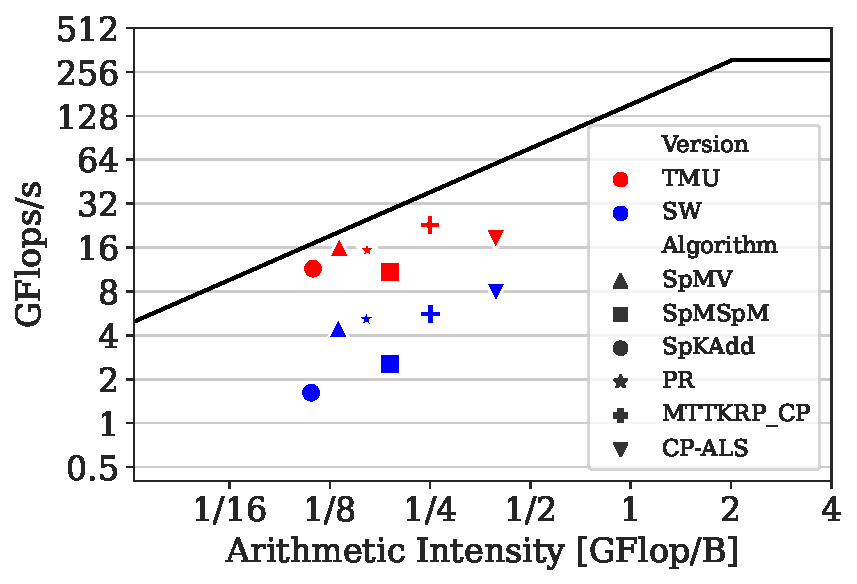
\includegraphics[width=\textwidth]{img_roofline_all.pdf}
        \vspace{-0.5cm}
        \caption{Geomean}
        \label{fig:tmu-scientific-roofline-geomean}
    \end{subfigure}
    \centering
    \begin{subfigure}[b]{0.48\textwidth}
        \centering
        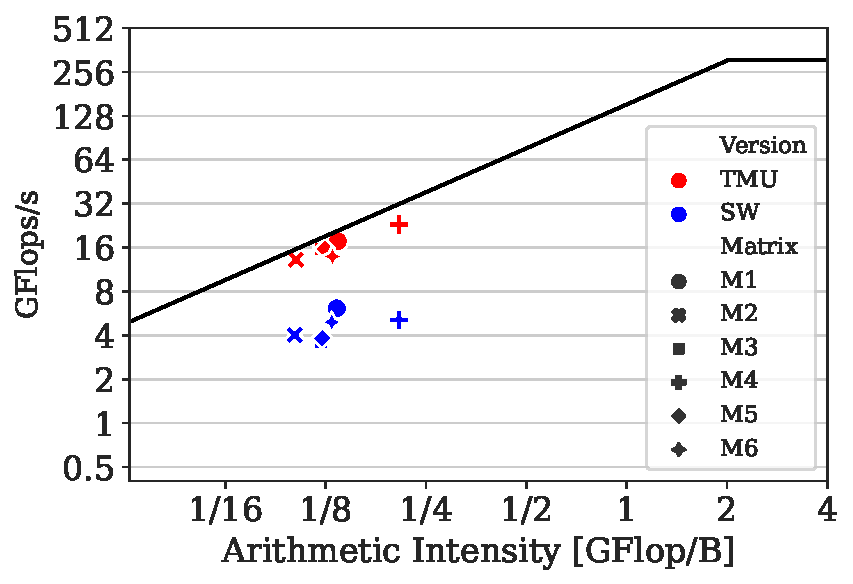
\includegraphics[width=\textwidth]{img_roofline_spmv.pdf}
        \vspace{-0.5cm}
        \caption{SpMV}
        \label{fig:tmu-scientific-roofline-spmv}
    \end{subfigure}
    \centering
    \begin{subfigure}[b]{0.48\textwidth}
        \centering
        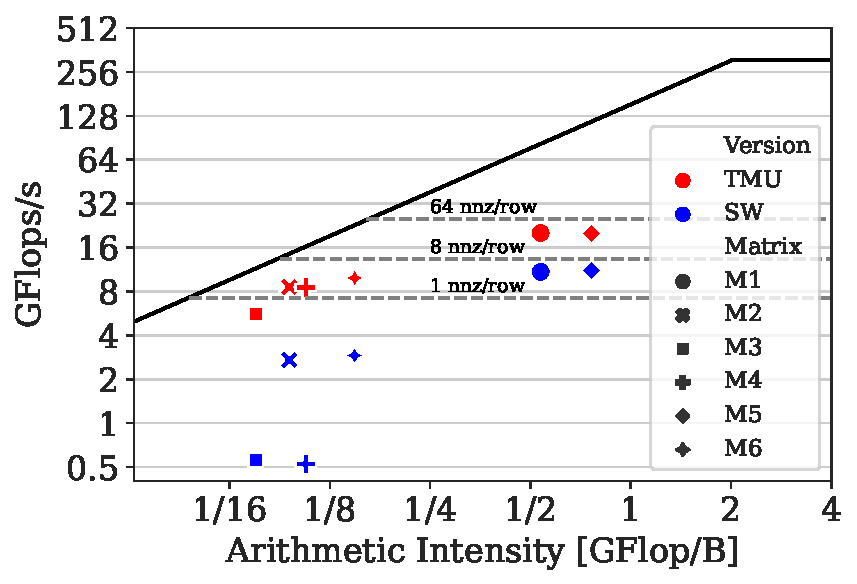
\includegraphics[width=\textwidth]{img_roofline_spgemm.pdf}
        \vspace{-0.5cm}
        \caption{SpMSpM}
        \label{fig:tmu-scientific-roofline-spmspm}
    \end{subfigure}
    \centering
    \begin{subfigure}[b]{0.48\textwidth}
        \centering
        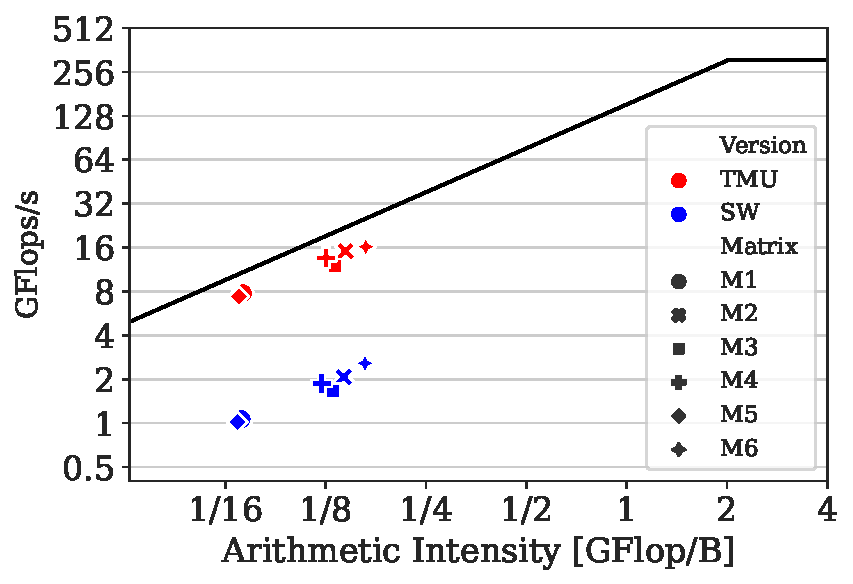
\includegraphics[width=\textwidth]{img_roofline_spkadd.pdf}
        \vspace{-0.5cm}
        \caption{SpKAdd}
        \label{fig:tmu-scientific-roofline-spkadd}
    \end{subfigure}
    \caption[Roofline models of a CPU and DAE processor on scientific kernels.]{Roofline analysis of the traditional CPU baseline and the proposed DAE processor on scientific sparse kernels. Both systems use the simulated multicore configuration in \Cref{tab:tmu-dae-system-specs}; the DAE processor augments each core with a TMU, while the baseline executes the optimized software implementations described in \Cref{sec:tmu-scientific-methodology}. Each point reports one execution, with operational intensity on the x-axis and achieved floating-point throughput on the y-axis; diagonal and horizontal roofs denote the memory-bandwidth and peak-compute limits, respectively. \Cref{fig:tmu-scientific-roofline-geomean} reports geomeans across inputs for each workload, while \Cref{fig:tmu-scientific-roofline-spmv,fig:tmu-scientific-roofline-spmspm,fig:tmu-scientific-roofline-spkadd} report all inputs for SpMV, SpMSpM, and SpKAdd; the dashed ceilings in \Cref{fig:tmu-scientific-roofline-spmspm} show idealized SpMSpM limits for fixed nonzeros per row. Overall, the TMU does not change operational intensity, but it moves executions closer to the relevant bandwidth or compute roof by improving memory-level parallelism and reducing traversal and merging overheads.}
    \label{fig:tmu-scientific-rooflines}
\end{figure}


To explain the improvements the TMU brings in terms of system utilization, we present Roofline models~\cite{roofline2009acm} in \Cref{fig:rooflines}. Roofline models relate arithmetic intensity (AI) (x-axis), measured by the ratio of total floating-point operations to total data movement, and performance in giga-flops (y-axis). The diagonal line draws the peak memory bandwidth, while the horizontal line is the processor's peak performance. 

\Cref{fig:roofline-geomean} shows the data points for the evaluated workloads with the geomean for all inputs, except TC (integer arithmetic) and SpTC (symbolic phase) that do not perform floating-point computation. As can be seen, baseline SVE software versions are unable to use a substantial amount of memory bandwidth, attaining poor system utilization and compute throughput. TMU-accelerated workloads are close to the memory bandwidth roof, and SpMV is almost saturating peak bandwidth, achieving significantly higher compute throughput. SpMSpM is unable to use as much bandwidth as the other workloads due to its compute-intensive nature.

The rest of the Roofline models focus on SpMV, SpMSpM, and SpKAdd, showing data for all inputs. For SpMV (\Cref{fig:roofline-spmv}), which is memory-intensive, the software version is not able to use the available memory bandwidth due to data-dependencies on long-latency memory accesses, quickly filling out-of-order core resources, stalling its execution. The dataflow design of the TMU unlocks additional MLP for offloaded traversals, increasing memory bandwidth utilization by almost 4$\times$, leading to much better system-level performance. A similar behavior can be observed in SpKAdd for the software baseline versions (\Cref{fig:roofline-spkadd}), where the additional pressure that merging puts on core resources leads to even lower performance. The TMU again enables almost close to peak bandwidth utilization, which combined with its merging support significantly boosts overall performance. 

Finally, for SpMSpM we also plot three additional dashed ceilings (\Cref{fig:roofline-spmspm}). We compute these ceilings by processing synthetic matrices, each one storing a fixed number of non-zeros per row ($n=\{1,8,64\}$) located at column indexes $\{0 .. n-1\}$, proxying performance on ideal spatio-temporal locality. The data points starting from the right correspond to inputs M5 and M1, respectively. These two matrices have higher nnzs per row values (see \Cref{tab:inputs}) and perform better on the software baseline with respect to other inputs due to higher AI. TMU-accelerated executions improve performance and bandwidth utilization, but the former is constrained by the inherent \emph{nnzs per row} compute ceilings.

\begin{figure}
    \centering
    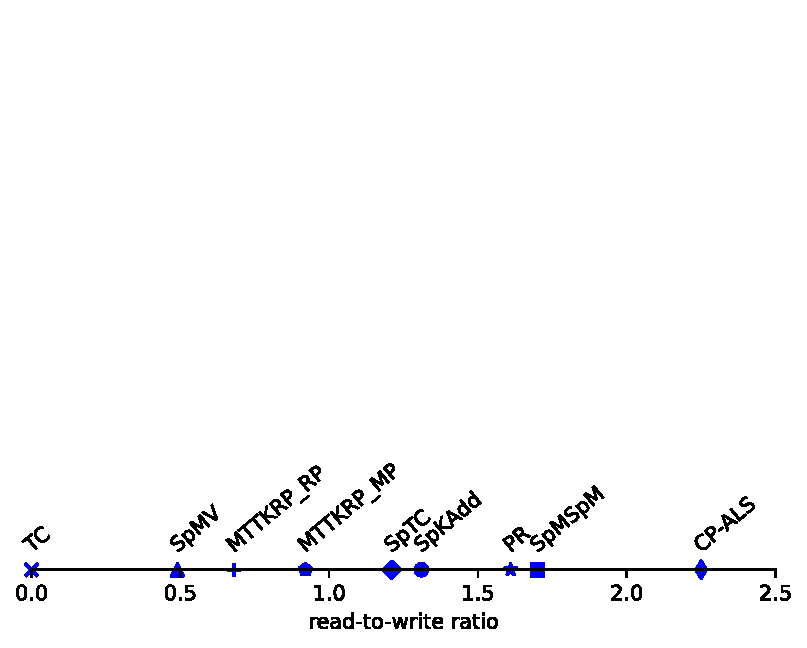
\includegraphics[width=.8\columnwidth]{img_read-to-write_plot-tilted.pdf}
    \caption[Read-to-write ratio of scientific workloads.]{Read-to-write ratio for evaluated workloads. The read-to-write ratio is the ratio between the time it takes the core to process (read) an outQ block versus the time it takes the TMU to produce (write) it. For simpler kernels with smaller compute (like SpMV), the core can read the queue and process data faster than the TMU loading data and writing it. As the read-to-write ratio is less than one, the TMU is the bottleneck. Instead, for more complex kernels like CP-ALS, the core is the bottleneck.}
    \label{fig:outq_rd2wr_ratio}
\end{figure}

The core and the TMU work in a decoupled pipelined manner. Therefore, we introduce the \textit{read-to-write ratio}, which is defined as the ratio between the time it takes the core to process (read) an outQ block versus the time it takes the TMU to produce (write) it, averaged over all blocks. \Cref{fig:outq_rd2wr_ratio} shows this ratio for the evaluated workloads. A value below one implies the core is faster than the engine. We observe this happens for TC, since merging is offloaded to the TMU, and for SpMV and MTTKRP, where the compute is very regular due to the SIMD-friendly data layout produced by the TMU. SpKAdd and SpTC have ratios close one, which indicates a balanced execution. SpMSpM, PR and CP-ALS have higher ratios due to more and less regular compute, indicating that the bottleneck is on the core's side.

Our evaluation demonstrates that the TMU successfully accelerates tensor traversals and merging operations, thereby improving overall system utilization. Moreover, performing computation on the core enables additional flexibility to seamlessly express and accelerate workloads that implement kernel fusion (TC) and that require evaluating partial results (CP-ALS).

%%%%%%%%%%%%%%%%%%%%%%%%%%%%%%%%%%%%%%%%%%%%%%%%%%%%%%%%%%%%%%%%%%%%%%%%%%%%%%%%%%%%%%%%%%%%%%%%%%%%%%%%%%%%%%%%%%%%%%%%%%%%%%%%%%%
\subsection{Sensitivity Analysis} %%%%%%%%%%%%%%%%%%%%%%%%%%%%%%%%%%%%%%%%%%%%%%%%%%%%%%%%%%%%%%%%%%%%%%%%%%%%%%%%%%%%%%%%%%%%%%%%%
%%%%%%%%%%%%%%%%%%%%%%%%%%%%%%%%%%%%%%%%%%%%%%%%%%%%%%%%%%%%%%%%%%%%%%%%%%%%%%%%%%%%%%%%%%%%%%%%%%%%%%%%%%%%%%%%%%%%%%%%%%%%%%%%%%%

\begin{figure}
    \centering
    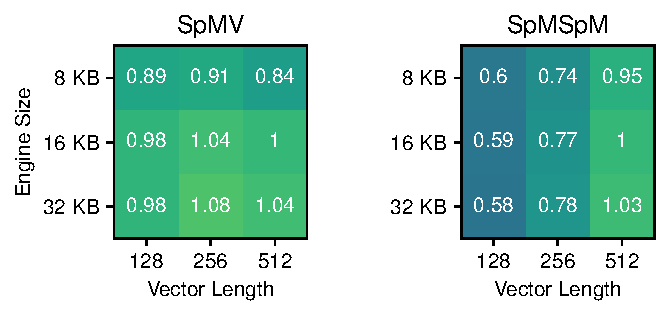
\includegraphics[width=.7\columnwidth]{img_dse_heatmap.pdf}
    \caption[Performance of different TMU configurations.]{Design space exploration varying engine storage size and SVE vector length.}
    \label{fig:dse}
\end{figure}

\Cref{fig:dse} shows a sensitivity analysis varying the total engine size and SVE vector length, which is tied to the number of TMU lanes. That is, a system with 512-bit SVE has an 8-lane TMU design, while a system with 256-bit SVE has a 4-lane TMU design. The heatmap shows normalized speedup with respect to the evaluated 16KB 512-bit SVE configuration. We observe that SpMV is more sensitive to engine storage, as larger storage enables more MLP, hiding memory latency, which is the main bottleneck in SpMV. SVE length does not have a large impact, since SpMV has a read-to-write ratio of 0.5. In SpMSpM we observe the opposite behavior: wider SVE length has a large performance impact, since the bottleneck is on the core side (1.68 read-to-write ratio).

%%%%%%%%%%%%%%%%%%%%%%%%%%%%%%%%%%%%%%%%%%%%%%%%%%%%%%%%%%%%%%%%%%%%%%%%%%%%%%%%%%%%%%%%%%%%%%%%%%%%%%%%%%%%%%%%%%%%%%%%%%%%%%%%%%%
\subsection{Comparison with the State of the Art} %%%%%%%%%%%%%%%%%%%%%%%%%%%%%%%%%%%%%%%%%%%%%%%%%%%%%%%%%%%%%%%%%%%%%%%%%%%%%%%%%
%%%%%%%%%%%%%%%%%%%%%%%%%%%%%%%%%%%%%%%%%%%%%%%%%%%%%%%%%%%%%%%%%%%%%%%%%%%%%%%%%%%%%%%%%%%%%%%%%%%%%%%%%%%%%%%%%%%%%%%%%%%%%%%%%%%

\begin{figure}
    \centering
    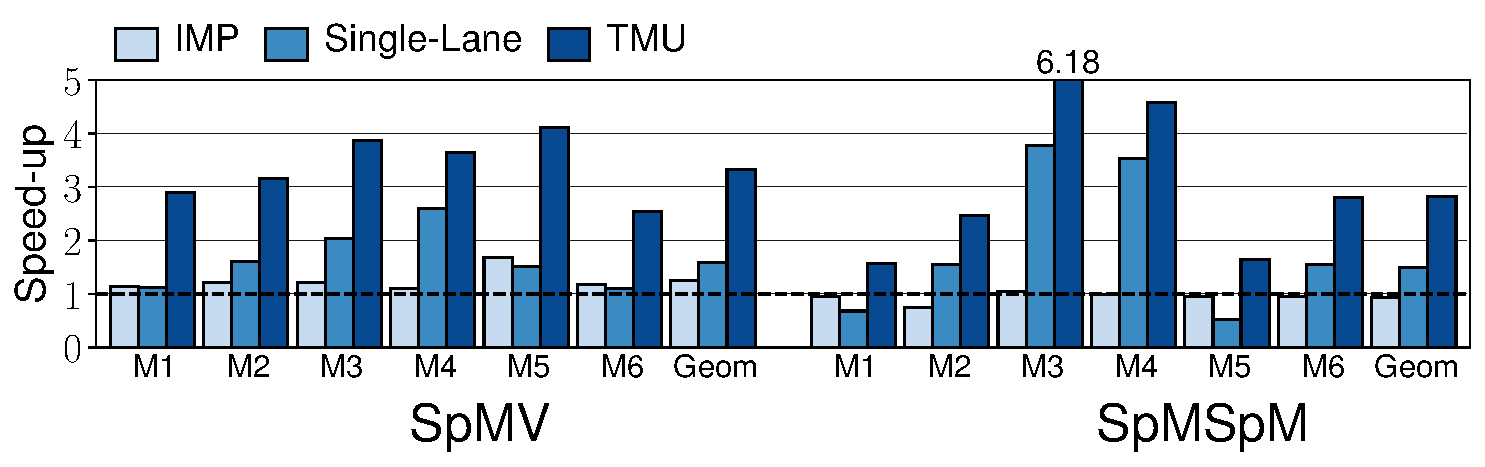
\includegraphics[width=.8\columnwidth]{img_imp_single_multi.pdf}
    \caption[TMU vs. other architectural solutions for accelerating scientific models.]{Speedup of different state-of-the-art solutions with respect to baseline. \emph{IMP} is the baseline plus the IMP prefetcher. \emph{Single-Lane} is the baseline plus a single-lane TMU per core (which proxies scalar vector engines in the literature). \emph{TMU} is the baseline plus full TMUs. with respect to baseline.}
    \label{fig:speedups_wrt_soa}
\end{figure}

Existing traversal engines integrated into multicore systems are conceived for graph analytics~\cite{spzip2021isca, hats}. For this reason, they feature architectures similar to a single TMU lane, but with fewer primitives (i.e., stream types) and no support for parallel data loading or merging, limiting their applicability to simple linear algebra kernels. Two prominent examples are HATS~\cite{hats} and SpZip~\cite{spzip2021isca}, the former exploits locality in graph communities and the latter implements de(compression) techniques. Both optimizations are orthogonal to the TMU operation. Therefore, we evaluate a \emph{Single-Lane} TMU with the same storage as the multi-lane \emph{TMU} employed throughout the evaluation. \Cref{fig:speedups_wrt_soa} shows that \emph{Single-Lane} achieves 1.59$\times$ and 1.50$\times$ geomean speedup on SpMV and SpMSpM, while \emph{TMU} gets 3.32$\times$ and 2.82$\times$, respectively. This indicates that traversal engines for graph analytics would benefit from parallel data loading as well.

We also evaluate the Indirect Memory Prefetcher (IMP)~\cite{yu2015}, configured as recommended by the authors of the paper, including the use of virtual address to prefetch across memory page boundaries. IMP performs well on SpMV, with an average speedup of 1.25$\times$, but fails to deliver performance improvements on SpMSpM due to thrashing of partial results. Overall, \emph{Single-Lane} and \emph{TMU} obtain better performance as they unlock more MLP which always fetches useful data.

%%%%%%%%%%%%%%%%%%%%%%%%%%%%%%%%%%%%%%%%%%%%%%%%%%%%%%%%%%%%%%%%%%%%%%%%%%%%%%%%%%%%%%%%%%%%%%%%%%%%%%%%%%%%%%%%%%%%%%%%%%%%%%%%%%%
\subsection{RTL Implementation and Area Analysis} %%%%%%%%%%%%%%%%%%%%%%%%%%%%%%%%%%%%%%%%%%%%%%%%%%%%%%%%%%%%%%%%%%%%%%%%%%%%%%%%
%%%%%%%%%%%%%%%%%%%%%%%%%%%%%%%%%%%%%%%%%%%%%%%%%%%%%%%%%%%%%%%%%%%%%%%%%%%%%%%%%%%%%%%%%%%%%%%%%%%%%%%%%%%%%%%%%%%%%%%%%%%%%%%%%%%
We implement the TMU in System Verilog using the parameters listed in \Cref{table:gem5} and synthesize the design using the GlobalFoundries 22nm FD-SOI technology node. We have used the Cadence Genus tool v19.11 for the logical synthesis and the Cadence Innovus tool v19.11 for the place-and-route. 
The standard cell libraries have 8-tracks, low Vt, and a 104 CPP. We have used high-performance dual-port SRAMs to implement the different data and metadata arrays inside the engine. 
The area cost of the TMU is $0.0704$mm$^2$, where each lane occupies just $0.0080$mm$^2$. The TMU requires 1.52\% of the area of a Neoverse N1 core~\cite{n1core}, the one modeled in our evaluation, when scaled to the same technology node~\cite{area-scaling}.
Moreover, the entire sparse engine is $0.5\times$ smaller than a 32 KB and 8-way L1 data cache in the 22nnm technology.

%%%%%%%%%%%%%%%%%%%%%%%%%%%%%%%%%%%%%%%%%%%%%%%%%%%%%%%%%%%%%%%%%%%%%%%%%%%%%%%%%%%%%%%%%%%%%%%%%%%%%%%%%%%%%%%%%%%%%%%%%%%%%%%%%%%
\section{The Potential of Accelerating Machine Learning Models with the TMU} \label{sec:dae-potential-machine-learning} %%%%%%%%%%%%%%%%%%%%%%%%%%%%
%%%%%%%%%%%%%%%%%%%%%%%%%%%%%%%%%%%%%%%%%%%%%%%%%%%%%%%%%%%%%%%%%%%%%%%%%%%%%%%%%%%%%%%%%%%%%%%%%%%%%%%%%%%%%%%%%%%%%%%%%%%%%%%%%%%

This section discusses how the TMU can accelerate the embedding operations in \Cref{sec:sparsity-in-machine-learning}.

%%%%%%%%%%%%%%%%%%%%%%%%%%%%%%%%%%%%%%%%%%%%%%%%%%%%%%%%%%%%%%%%%%%%%%%%%%%%%%%%%%%%%%%%%%%%%%%%%%%%%%%%%%%%%%%%%%%%%%%%%%%%%%%%%%%
\subsection{Experimental Methodology} %%%%%%%%%%%%%%%%%%%%%%%%%%%%%%%%%%%%%%%%%%%%%%%%%%%%%%%%
%%%%%%%%%%%%%%%%%%%%%%%%%%%%%%%%%%%%%%%%%%%%%%%%%%%%%%%%%%%%%%%%%%%%%%%%%%%%%%%%%%%%%%%%%%%%%%%%%%%%%%%%%%%%%%%%%%%%%%%%%%%%%%%%%%%

%+++++++++++++++++++++++++++++++++++++++++++
%++++++++++ START TMU HW OVERVIEW ++++++++++
%+++++++++++++++++++++++++++++++++++++++++++
\begin{figure}
\centering
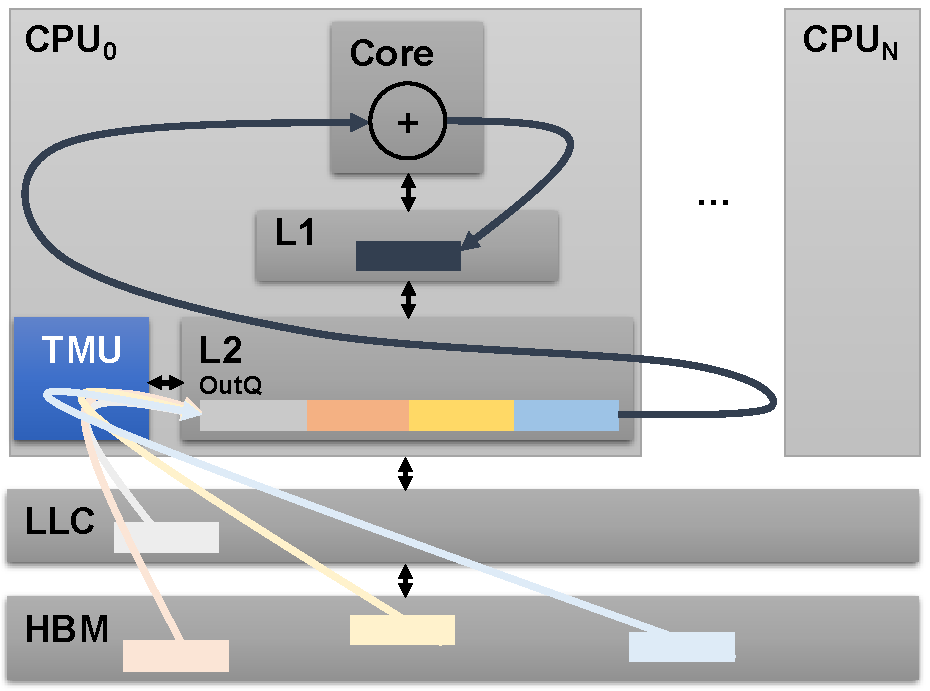
\includegraphics[width=0.55\linewidth]{img_dae_system.pdf} % L B R T
\caption[Visualization of an embedding operation on a DAE processor.]{Our DAE processor---a traditional multicore processor (same as \Cref{tab:cpu-specs-embedding}) featuring one TMU per core to offload embedding lookups. Each TMU has 8KB storage, 256 MSHRs, and runs at 1 GHz. The TMU loads embedding vectors from either HBM or LLC, and marshals them in the private L2 cache of the core, which accumulates them with SVE units and stores partial results in private L2 cache.}
\label{fig:dae-processor}
\end{figure}
%+++++++++++++++++++++++++++++++++++++++++
%++++++++++ END TMU HW OVERVIEW ++++++++++
%+++++++++++++++++++++++++++++++++++++++++


\Cref{fig:dae-processor} shows the DAE system we used in this study, and how embedding operations are executed. Similarly to \Cref{sec:architectural-implications-of-sparsity}, such DAE system is the DAE processor in \Cref{tab:cpu-specs-embedding} featuring one TMU per core to offload embedding lookups. The experimental methodology for GPU also follows \Cref{sec:architectural-implications-of-sparsity}, and GPU power consumption is measured with the \texttt{torch.cuda.power\_draw} function.

%%%%%%%%%%%%%%%%%%%%%%%%%%%%%%%%%%%%%%%%%%%%%%%%%%%%%%%%%%%%%%%%%%%%%%%%%%%%%%%%%%%%%%%%%%%%%%%%%%%%%%%%%%%%%%%%%%%%%%%%%%%%%%%%%%%
\subsection{Architectural Advantage of DAE Designs} \label{sec:architectural-advantages-of-dae-designs} %%%%%%%%%%%%%%%%%%%%%%%%%%%%%%%%%%%%%%%%%%%%%%%%%%%%%%%%
%%%%%%%%%%%%%%%%%%%%%%%%%%%%%%%%%%%%%%%%%%%%%%%%%%%%%%%%%%%%%%%%%%%%%%%%%%%%%%%%%%%%%%%%%%%%%%%%%%%%%%%%%%%%%%%%%%%%%%%%%%%%%%%%%%%

%+++++++++++++++++++++++++++++++++++++++++
%+++++++++++++ START MISS BW +++++++++++++
%+++++++++++++++++++++++++++++++++++++++++
\begin{figure}
\centering
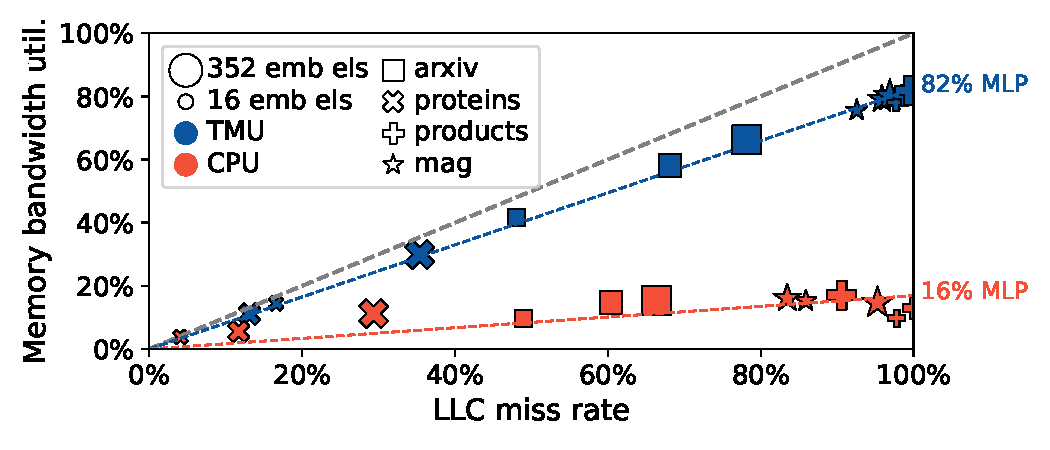
\includegraphics[width=.8\linewidth]{img_bw_per_miss.pdf} 
\vspace{-1em}
\caption[TMU and CPU memory-level parallelism for graph convolution.]{TMU and CPU memory bandwidth utilization for graph convolutions in different GNN layers. The x-axis indicates their LLC miss rates. Dashed lines are the Memory-Level Parallelism (MLP) calculated with linear regression on Little's rule~\cite{little1961queue}. The bold dashed gray line is the ideal MLP. Overall, the TMU enables higher memory-level parallelism, and larger memory-bandwidth utilization.}
\label{fig:bw-per-miss}
%\vspace{-0.5em}
\end{figure}
%+++++++++++++++++++++++++++++++++++++++
%+++++++++++++ END MISS BW +++++++++++++
%+++++++++++++++++++++++++++++++++++++++

%+++++++++++++++++++++++++++++++++++++++++++++++++
%++++++++++ START DAE IMPROVEMENT TOTAL ++++++++++
%+++++++++++++++++++++++++++++++++++++++++++++++++
\begin{figure}
\centering
    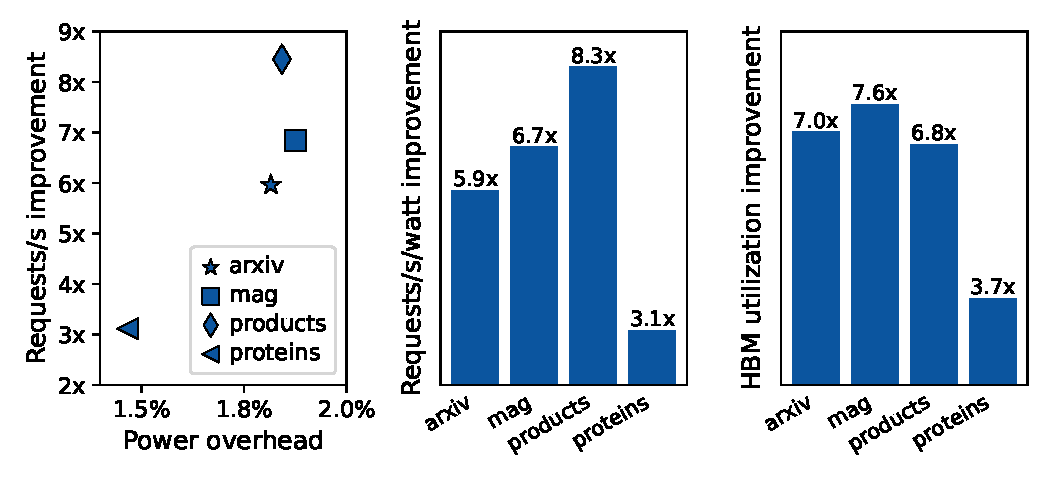
\includegraphics[width=\linewidth]{img_dae_impact.pdf}
    %\vspace{-1em}
    \begin{subfigure}[b]{0.325\linewidth} % 40% width
        \vspace{-5em}
        \caption{}
        \label{fig:ppw-scatter-plot}
    \end{subfigure}
    \begin{subfigure}[b]{0.325\linewidth} % 40% width
        \vspace{-5em}
        \caption{}
        \label{fig:ppw-dae-improvement}
    \end{subfigure}
    \begin{subfigure}[b]{0.325\linewidth} % 40% width
        \vspace{-5em}
        \caption{}
        \label{fig:hbm-dae-improvement}
    \end{subfigure}
    %\vspace{-1em}
    \caption[Performance and efficiency of a DAE core over a traditional core on graph convolutions.]{Performance and efficiency of a DAE core over a traditional core on graph convolutions. The leftmost plot (a) shows the throughput improvement (in requests/second) given by the TMU, compared to its overhead in power consumption. The middle plot (b) shows the requests per second per watt improvement given by the TMU. The rightmost plot (c) shows the improvement in memory bandwidth given by the TMU. Overall, access units like the TMU can issue and track more memory requests at low power consumption (a). In this way, they can achieve high efficiency (b) and HBM utilization (c).}
    \label{fig:dae-advantage}
\end{figure}
%+++++++++++++++++++++++++++++++++++++++++
%++++++++++ END DAE IMPROVEMENT ++++++++++
%+++++++++++++++++++++++++++++++++++++++++

%++++++++++++++++++++++++++++++++++++++++++++
%+++++++++++++ START BW SCALING +++++++++++++
%++++++++++++++++++++++++++++++++++++++++++++
\begin{figure}
\centering
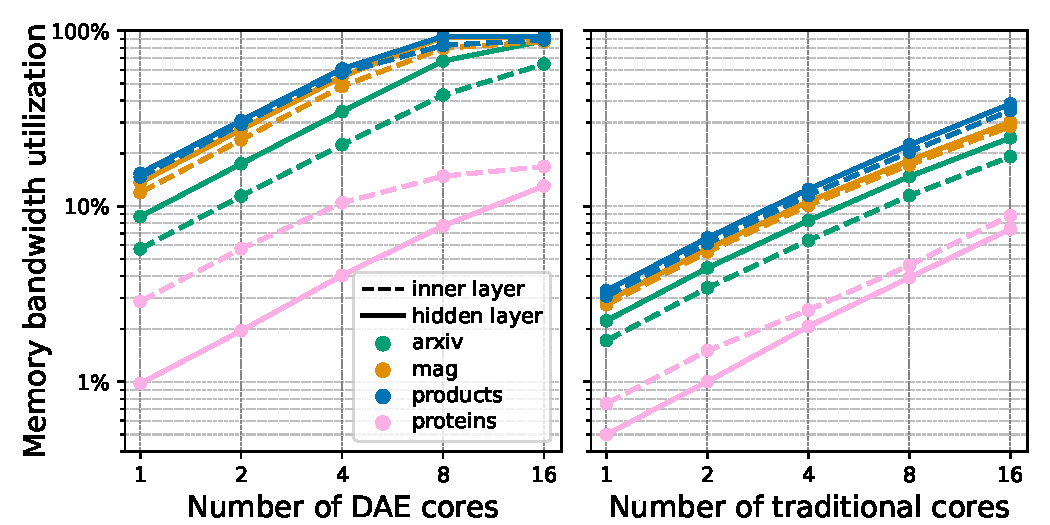
\includegraphics[width=.8\linewidth]{img_bw_scaling.pdf} 
%\vspace{-1em}
\caption[Bandwidth scaling of DAE cores vs traditional cores for graph convolution.]{Bandwidth utilization of a single HBM stack when scaling traditional cores and DAE cores. Different colors denote different inputs. Dashed lines are input layers (generally having smaller embeddings). Solid lines are hidden layers (generally having larger embeddings). Overall, DAE architectures (1)~achieve higher performance with the same core count, and (2)~require fewer cores to achieve same performance, achieving higher efficiency.}
\label{fig:bw-scaling}
%\vspace{-0.5em}
\end{figure}
%++++++++++++++++++++++++++++++++++++++++++
%+++++++++++++ END BW SCALING +++++++++++++
%++++++++++++++++++++++++++++++++++++++++++

The main advantage of DAE designs is that, by decoupling embedding lookup and computation into two distinct units, these units can be specialized and optimized independently.

For instance, as the TMU implements all the logic to traverse and load tensor operands using specialized dataflow hardware, it can issue memory requests with higher throughput and efficiency than the core. Moreover, as the TMU can run at a lower frequency, it can track 8$\times$ more outstanding requests, with no timing issues, and low power consumption (less than 2\% overhead, as in \Cref{sec:dae-potential-scientific}). \Cref{fig:bw-per-miss} demonstrates that the TMU can track 82\% of the outstanding memory requests required to achieve full throughput (one request per cycle), whereas the CPU only 16\%. Hence, as shown in \Cref{fig:ppw-scatter-plot} and \ref{fig:ppw-dae-improvement}, the TMU achieves 5.7$\times$ and 5.6$\times$ higher requests/s and requests/s/watt than traditional cores, 5.2$\times$ and 6.3$\times$ better than doubling core's outstanding requests (\Cref{fig:dse-cpu}). In this way, as shown in \Cref{fig:hbm-dae-improvement}, the TMU utilizes 4$\times$---8$\times$ more memory bandwidth than a traditional core. Hence, as shown in \Cref{fig:bw-scaling}, DAE architectures (1)~achieve higher performance with the same core count, and (2)~require fewer cores to achieve same performance, achieving higher efficiency.

%%%%%%%%%%%%%%%%%%%%%%%%%%%%%%%%%%%%%%%%%%%%%%%%%%%%%%%%%%%%%%%%%%%%%%%%%%%%%%%%%%%%%%%%%%%%%%%%%%%%%%%%%%%%%%%%%%%%%%%%%%%%%%%%%%%
\subsection{DAE Processor vs. CPU} \label{sec:dae-vs-cpu} %%%%%%%%%%%%%%%%%%%%%%%%%%%%%%%%%%%%%%%%%%%%%%%%%%%%%%%%
%%%%%%%%%%%%%%%%%%%%%%%%%%%%%%%%%%%%%%%%%%%%%%%%%%%%%%%%%%%%%%%%%%%%%%%%%%%%%%%%%%%%%%%%%%%%%%%%%%%%%%%%%%%%%%%%%%%%%%%%%%%%%%%%%%%

%+++++++++++++++++++++++++++++++++++++++++
%++++++++++ START SPEEDUP TOTAL ++++++++++
%+++++++++++++++++++++++++++++++++++++++++
\begin{figure}
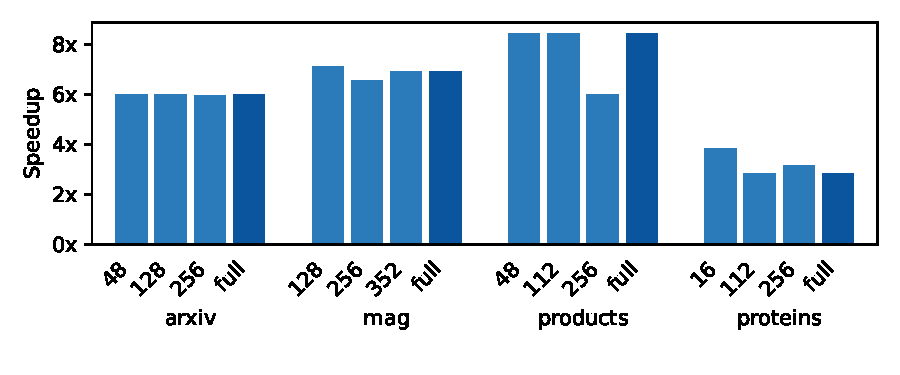
\includegraphics[width=\linewidth]{img_gnn_speedups.pdf} 
\vspace{-3em}
\caption[Performance potential of TMU on graph convolution.]{Performance speedup of graph convolutions when offloading embedding lookup to a near-core access unit like the TMU. Baseline is traditional CPU. Lighter bars are the speedup of each layer (and its embedding size), and the darker is the overall speedup of all the layers.}
\label{fig:speedups-wrt-cpu}
%\vspace{-0.5em}
\end{figure}
%+++++++++++++++++++++++++++++++++++++++
%++++++++++ END SPEEDUP TOTAL ++++++++++
%+++++++++++++++++++++++++++++++++++++++

%+++++++++++++++++++++++++++++++++++++++++
%++++++++++ START SPEEDUP TOTAL ++++++++++
%+++++++++++++++++++++++++++++++++++++++++
\begin{figure}
\centering
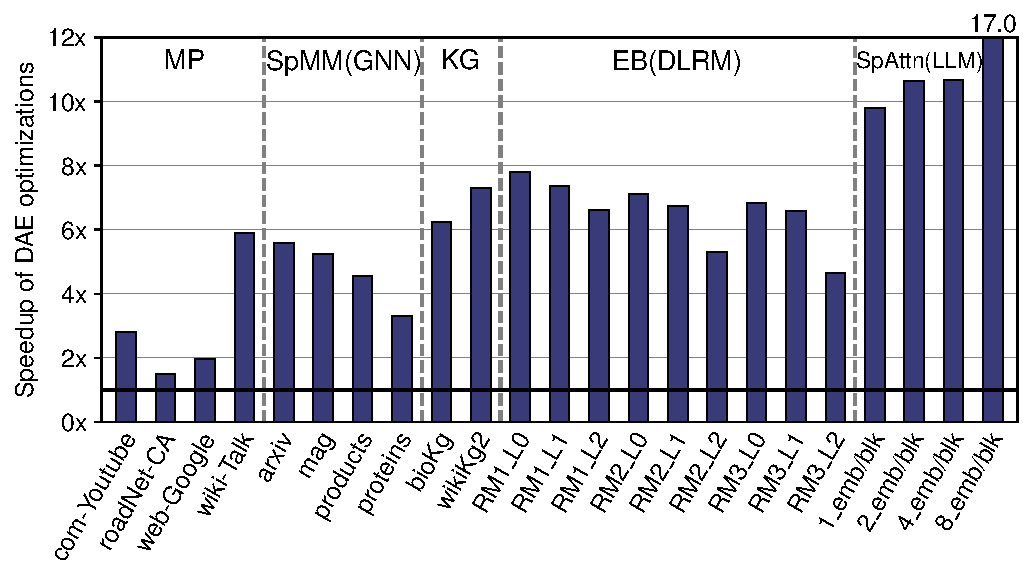
\includegraphics[width=.8\linewidth]{img_dae_speedups.pdf} 
\caption[Performance potential of TMU on all graph models.]{Performance benefit of offloading embedding lookup to a near-core access unit like the TMU. For graph-learning models, the inputs and feature sizes are reported in \Cref{tab:graph-inputs}. For DLRMs, we tested the three configurations in~\Cref{tab:dlrm-configurations}, each one running inputs with low (\texttt{L0}), medium (\texttt{L1}), and high (\texttt{L2}) locality~\cite{dlrm2020hpca}. For LLMs, we tested the original BigBird setting~\cite{bigbird2024neurips} while varying the blocks sizes. Overall, offloading lookup to a specialized access unit improves performance of embedding operations by 5.8$\times$.}
\label{fig:speedups-wrt-cpu-all}
\end{figure}
%+++++++++++++++++++++++++++++++++++++++
%++++++++++ END SPEEDUP TOTAL ++++++++++
%+++++++++++++++++++++++++++++++++++++++

From the core's perspective, offloading embedding lookup allows to fully utilize the core's resources for compute operations like embedding reductions. In the end, as shown in \Cref{fig:speedups-wrt-cpu}, decoupling embedding lookup from computation on multicore processors achieves a 2.9---8.2$\times$ speedup on GNN embedding operations, with speedups mostly proportional to their spatio-temporal locality. Moreover, as shown in \Cref{fig:speedups-wrt-cpu-all}, this also improves performance by an average 5.8$\times$ across all embedding operations in \Cref{sec:characterization-and-implications}.

%%%%%%%%%%%%%%%%%%%%%%%%%%%%%%%%%%%%%%%%%%%%%%%%%%%%%%%%%%%%%%%%%%%%%%%%%%%%%%%%%%%%%%%%%%%%%%%%%%%%%%%%%%%%%%%%%%%%%%%%%%%%%%%%%%%
\subsection{DAE Processor vs. GPU} \label{sec:dae-vs-gpu} %%%%%%%%%%%%%%%%%%%%%%%%%%%%%%%%%%%%%%%%%%%%%%%%%%%%%%%%
%%%%%%%%%%%%%%%%%%%%%%%%%%%%%%%%%%%%%%%%%%%%%%%%%%%%%%%%%%%%%%%%%%%%%%%%%%%%%%%%%%%%%%%%%%%%%%%%%%%%%%%%%%%%%%%%%%%%%%%%%%%%%%%%%%%


%++++++++++++++++++++++++++++++++++++++++++
%++++++++++ START GPU COMPARISON ++++++++++
%++++++++++++++++++++++++++++++++++++++++++
\begin{figure}
    \centering
    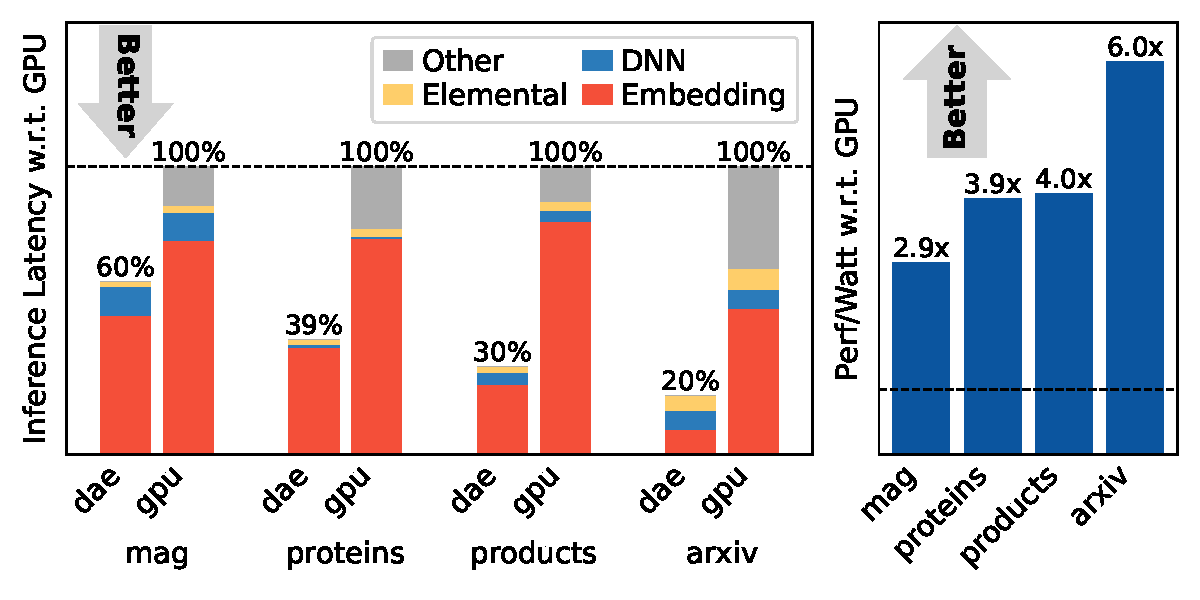
\includegraphics[width=\linewidth]{img_gpu_comparison.pdf}
    %\vspace{-1em}
    \begin{subfigure}[b]{0.7\linewidth} % 40% width
        \vspace{-2.5em}
        \caption{}
        \label{fig:gpu-perf}
    \end{subfigure}
    \begin{subfigure}[b]{0.25\linewidth} % 40% width
        \vspace{-2.5em}
        \caption{}
        \label{fig:gpu-ppw}
    \end{subfigure}
    %\vspace{-1em}
    \caption[Performance and efficiency of DAE processors vs. GPUs on GNNs.]{Performance and efficiency comparison of DAE processors w.r.t. GPUs on end-to-end GNNs models. The leftmost plot (a) shows inference latency of our DAE system and GPU. Goups of bars are inputs. The leftmost bar in the group is the inference latency of the DAE processor with respect to GPU, which is the rightmost bar. Each bar shows the breakdown across embedding operations, DNNs, elemental operations, and other operations. All operations---including graph convolution and neural networks---are either run on the DAE processor or on GPU. Instead, the rightmost plot is perforamnce per watt of the DAE processor compared to GPU. Overall, DAE processors can perform embedding operations substantially faster than GPUs, outperforming them on both inference latency and performance/watt.}
    \label{fig:gpu-comparison}
\end{figure}
%++++++++++++++++++++++++++++++++++++++++
%++++++++++ END GPU COMPARISON ++++++++++
%++++++++++++++++++++++++++++++++++++++++

\Cref{fig:gpu-perf} shows the inference latency breakdown of GNN models on the DAE processor and GPU. Although the two systems have the same peak memory bandwidth, the DAE system utilizes 4.6$\times$ higher bandwidth, executing embedding operations 1.8$\times$ faster than the GPU. Hence, the DAE processor achieves 2.9$\times$ higher end-to-end performance than the GPU. As the DAE processor saturates memory bandwidth with only 8---16 cores per HBM stack, it consumes less power than the GPU, and achieves 4.1$\times$ higher performance/watt, as shown in \Cref{fig:gpu-ppw}.

%%%%%%%%%%%%%%%%%%%%%%%%%%%%%%%%%%%%%%%%%%%%%%%%%%%%%%%%%%%%%%%%%%%%%%%%%%%%%%%%%%%%%%%%%%%%%%%%%%%%%%%%%%%%%%%%%%%%%%%%%%%%%%%%%%%
\subsection{Specialized DAE Architectures} \label{sec:PNM} %%%%%%%%%%%%%%%%%%%%%%%%%%%%%%%%%%%%%%%%%%%%%%%%%%%%%%%%
%%%%%%%%%%%%%%%%%%%%%%%%%%%%%%%%%%%%%%%%%%%%%%%%%%%%%%%%%%%%%%%%%%%%%%%%%%%%%%%%%%%%%%%%%%%%%%%%%%%%%%%%%%%%%%%%%%%%%%%%%%%%%%%%%%%

While the previous section demonstrates the potential of decoupling memory access from computation for optimizing a general-purpose processor, this section explores how that optimization enables more specialized architectures tailored for embedding operations.

\subsubsection{Motivation} \label{sec:pnm-motivation}

\begin{figure}
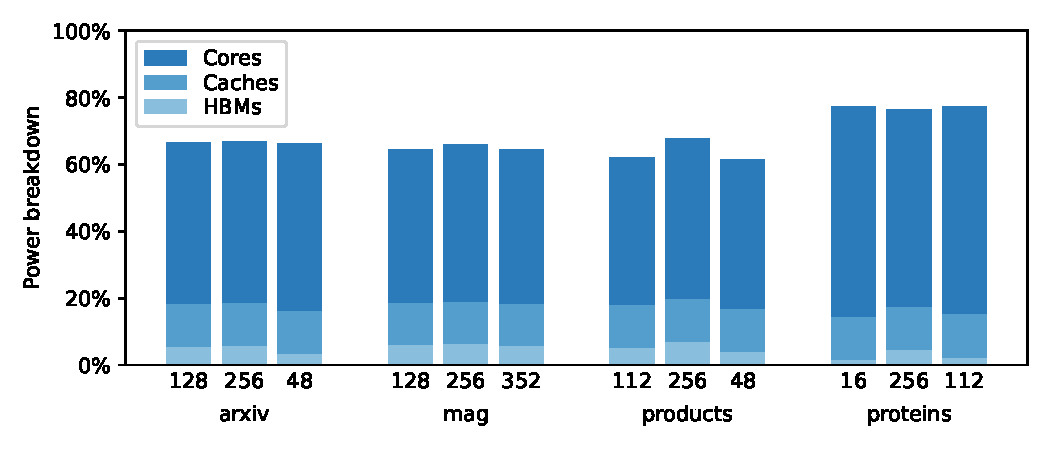
\includegraphics[width=\linewidth]{img_power_breakdown.pdf}
\vspace{-2em}
\caption[Power breakdown of our DAE processor for graph convolution.]{Power breakdown of our DAE processor, normalized to TDP. Each group corresponds to a dataset, and bars within a group represent different embedding sizes. Overall, more than 75\% of the power is consumed by compute cores and caches (excluding TMU).}
\label{fig:power-breakdown}
\end{figure}

\begin{figure}
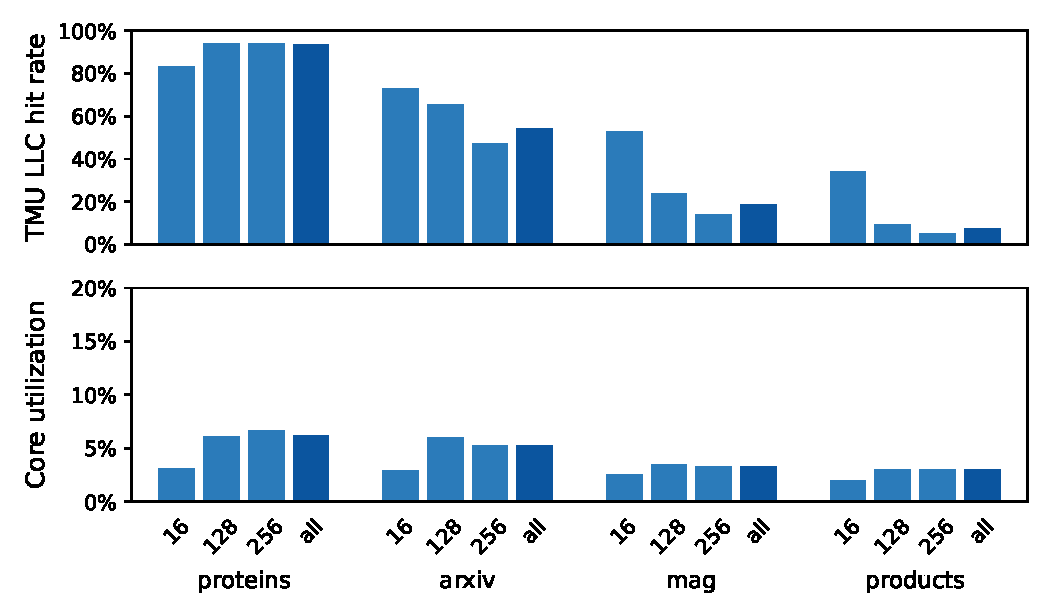
\includegraphics[width=\linewidth]{img_util_bars.pdf}
\vspace{-2em}
\caption[Compute and cache utilization of our DAE processor for graph convolution.]{Utilization of compute cores (achieved vs. peak FLOPs) and last-level cache (hit rate) for our DAE processor. Datasets are sorted by decreasing reuse, and bars represent embedding sizes. Compute utilization remains below 7\%, while cache effectiveness degrades significantly for larger embeddings and low-reuse datasets (down to 5\%).}
\label{fig:util-bars}
\end{figure}

The DAE processor described in the previous section is based on a conventional multicore design, augmented with a TMU per core to offload embedding lookups. While this approach improves performance and efficiency with minimal architectural changes, it does not fully exploit the specialization opportunities enabled by the TMU.

As shown in \Cref{fig:power-breakdown}, more than 75\% of the processor power is consumed by compute cores and associative caches. However, these components are overprovisioned for embedding workloads, where computation is limited to simple vector accumulation. Furthermore, as discussed earlier, caches are only effective if the input dataset has high reuse. Consequently, both compute and cache resources can be significantly underutilized, as illustrated in \Cref{fig:util-bars}.

Motivated by these observations, in this section we explore two complementary optimizations: (i) reducing the complexity of DAE compute cores to improve energy efficiency, and (ii) moving these simplified cores closer to memory to bypass the cache hierarchy.

\subsubsection{Experimental Setting} \label{sec:pnm-setting}

\begin{table}[]
\caption[Specifications of DAE big and little cores.]{DAE big and little cores. The TMU configuration remains unchanged; only compute resources differ.}
\label{tab:cores-specs}
\begin{tabular}{|c|c|c|}
\hline
                      & \textbf{Big}         & \textbf{Little}      \\ \hline
\textbf{Type}         & Arm N1-like          & Arm E1-like          \\ \hline
\textbf{Frequency}    & 2.4 GHz              & 1.2 GHz              \\ \hline
\textbf{Vector FLOPs} & 2 $\times$ 64B       & 2 $\times$ 16B       \\ \hline
%\textbf{ROB entries}  & 224                  & 40                   \\ \hline
%\textbf{LSQ entries}  & 2 $\times$ 96        & 2 $\times$ 8         \\ \hline
\textbf{TMU MLP}      & 256 requests         & 256 requests         \\ \hline
\end{tabular}
\end{table}

\begin{table}[]
\caption{Specialized DAE configurations.}
\label{tab:configurations}
\begin{tabular}{|c|c|c|}
\hline
            & \textbf{DAE host cores}                                                           & \textbf{DAE mem cores}                                                          \\ \hline
\textbf{BH} & TMU+Big compute                                                                   & None                                                                            \\ \hline
\textbf{LH} & TMU+Little compute                                                                & None                                                                            \\ \hline
\textbf{LM} & \begin{tabular}[c]{@{}c@{}}TMU+Little compute\\ (for reduce-scatter)\end{tabular} & \begin{tabular}[c]{@{}c@{}}TMU+Little compute\\ (for embedding op)\end{tabular} \\ \hline
\end{tabular}
\end{table}

We name configurations based on whether embedding operations are executed on big (\texttt{B}) or little (\texttt{L}) DAE cores, located either in the host processor (\texttt{H}) or near memory (\texttt{M}). Each DAE core consists of a TMU paired with either a big or little compute core, as described in \Cref{tab:cores-specs}.

Our baseline is our high-performance DAE multicore processor, denoted \texttt{dae-bh}. The \texttt{dae-lh} configuration replaces big cores with little cores while preserving core count, TMU capacity, and memory hierarchy. The \texttt{dae-lm} configuration extends \texttt{dae-lh} by placing eight little DAE cores in the base die of each Processing Near HBM (PN-HBM) stack. \Cref{tab:configurations} summarizes these configurations.

The \texttt{dae-lm} system includes six PN-HBM devices, each treated as an accelerator with a private address space. The remaining processor components (cache hierarchy and host DAE cores) form the host CPU. We distribute work across PN-HBM devices using row parallelism~\cite{dlrm2022mudigere}, where embedding tables are sharded by rows and mapped across memory stacks. Each device processes its partition independently, and partial results are combined via a \texttt{reduce-scatter} operation, performed on the host CPU while PN-HBM devices execute embedding operations.

As before, we evaluate performance and power using gem5~\cite{lowepower2020gem5} and McPAT~\cite{li2009mcpat} for the host CPU, and Ramulator2.0~\cite{ramulator2016cs} for PN-HBM modeling.

\subsubsection{Results}

\begin{figure}
\centering
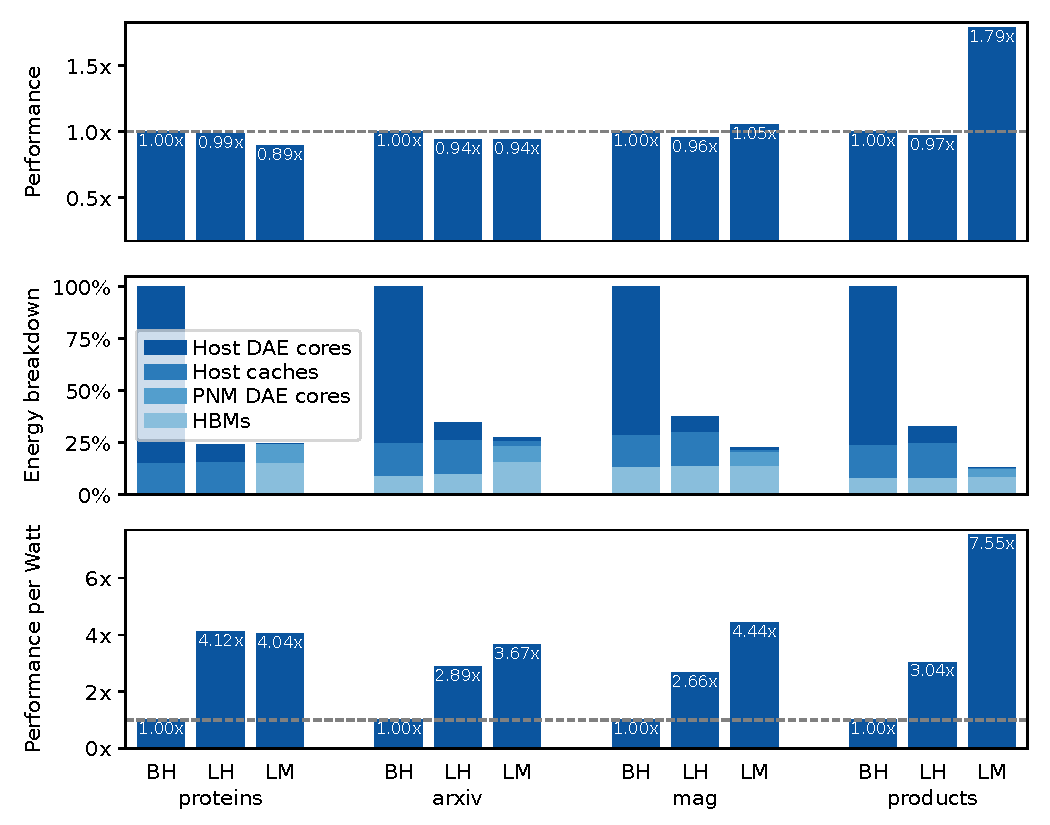
\includegraphics[width=\linewidth]{img_pim_comparison_bars.pdf}
\vspace{-2.2em}
\caption[Performance and efficiency of specialized DAE configurations.]{Performance, energy breakdown, and performance-per-watt improvements across specialized DAE configurations. Datasets are sorted by decreasing reuse. Using smaller DAE cores (\texttt{dae-lh}) significantly reduces power with minimal performance loss, while near-memory execution (\texttt{dae-lm}) further benefits low-reuse workloads.}
\label{fig:pim-speedups}
\end{figure}

\Cref{fig:pim-speedups} summarizes the performance and efficiency impact of the proposed optimizations. Overall, reducing compute core complexity (\texttt{dae-lh}) substantially improves energy efficiency with minimal performance degradation, while near-memory execution (\texttt{dae-lm}) provides additional gains for low-reuse workloads.

The \texttt{dae-lh} configuration achieves 94\%–99\% of the performance of \texttt{dae-bh}, while improving performance per watt by 2.66$\times$–4.12$\times$. This is because embedding operations underutilize large out-of-order cores (\Cref{sec:pnm-motivation}), and simpler cores can deliver comparable throughput at only 10\%–12\% of the energy. Workloads with higher node degree achieve better performance due to increased computation per memory access, while low-reuse workloads exhibit lower efficiency due to dominant memory and cache overheads.

In contrast, \texttt{dae-lm} provides the highest benefits for low-reuse datasets, where caches are ineffective. By moving DAE cores closer to memory, this configuration eliminates unnecessary cache accesses, reducing both latency and energy. For example, on \texttt{products}, \texttt{dae-lm} achieves 1.85$\times$ higher performance and 4.39$\times$ higher efficiency than \texttt{dae-lh}, and 1.79$\times$ higher performance and 7.86$\times$ higher efficiency than \texttt{dae-bh}. Similar trends are observed for \texttt{mag}, where \texttt{dae-lm} improves performance by 9\% and efficiency by 83\% over \texttt{dae-lh}.

These gains stem from eliminating cache overheads, which account for up to 50\% of total energy in low-reuse workloads. However, for higher-reuse workloads, caches remain beneficial. For example, on \texttt{arxiv}, \texttt{dae-lm} is slightly slower (1\%) but 1.46$\times$ more efficient than \texttt{dae-lh}. On \texttt{proteins}, where most accesses are cacheable, \texttt{dae-lm} is both slower and less efficient due to increased memory traffic. In this case, \texttt{dae-lh} achieves 21\% higher performance and slightly better efficiency.

Overall, \texttt{dae-lh} is preferable for high-reuse workloads, while \texttt{dae-lm} is better suited for low-reuse workloads.

\section{Summary}

In this chapter, we have demonstrated that DAE architectures that decouple memory access from computation achieve higher performance and efficiency. However, this optimization requires a more complex programming model, and a compiler, as explained in the next chapter.